% concatenated from main.tex
\documentclass[oneside,reqno]{amsart}
%\documentclass[]{amsart}
\usepackage[T1]{fontenc}		%%% T1 font encoding for accents
\usepackage{ankita-packages}
\usepackage{ankita-commands}
\usepackage{ankita-thms}
\usepackage{ankita-spacing}
\usepackage{combgames}
\usepackage{scrextend}          %%%to use addmargin
\usepackage{bm}
\usepackage[table]{xcolor}
%\usepackage[clipbox=false]{adjustbox}
\usetikzlibrary{positioning,decorations.pathreplacing}
\usepackage{mathrsfs}
\newcommand{\ur}[1]{\textcolor{blue}{#1}}
\newcommand{\an}[1]{\textcolor{red}{#1}}
\newcommand{\nir}[1]{\textcolor{purple}{#1}}
\newcommand{\fs}{\mathcal{F}}
\newcommand{\ts}{\mathcal{T}}
% \newcommand{\cgfarstar}{\cgfarstar}
\newcommand{\aw}{\mathrm{aw}}
\newcommand{\lp}{\mathscr{L}}
\newcommand{\rp}{\mathscr{R}}
\newcommand{\np}{\mathscr{N}}
\newcommand{\pp}{\mathscr{P}}
\newcommand{\hbeta}{\widehat\beta}
\newcommand{\rc}{\cellcolor{red!25}}
\newcommand{\bc}{\cellcolor{blue!40}}
\newcommand{\gc}{\cellcolor{green!40}}
\newtheorem{theoremm}{Theorem~2.3}

\usetikzlibrary {shapes.geometric}
\tikzset{star/.pic={
        % Code for a "plus".
        \node [star, star point ratio=.08cm, draw, scale=0.4] at (0,0) { };
        }}
\newcommand{\cgfarstareq}[2]{{#1}\sim_{\cgfarstar}{#2}}
\makeatletter
\@namedef{subjclassname@2020}{\textup{2020} Mathematics Subject Classification}
\makeatother

\title{Partizan Subtraction with full and truncated support}



\author[Ankita Dargad]{Ankita Dargad}
\address{Department of Mathematics, Indian Institute of Technology Bombay, Powai, Mumbai 400076}
\email{ankitadargad.iitb@gmail.com}

\author[U. Larsson]{Urban Larsson}
\address{Department of Industrial Engineering and Operations Research, Indian Institute of Technology Bombay, Powai, Mumbai 400076}
\email{larsson@iitb.ac.in}

\subjclass[MSC 2020]{Primary 91A46; Secondary 91A05} % Replace with appropriate MSC codes
\keywords{Combinatorial Game, Partizan Subtraction, Atomic Weight, Domination, Balance, Wealth Nim}
% \subjclass[2020]{Primary 05C15; Secondary 05C10, 05C35, 05C75}
% \keywords{Wealth Nim, Temperature theory, Pingala Sequence, Golden Ratio}

\date{\today}

\begin{document}
\begin{abstract}
    We investigate {\sc Full Support (FS)}, a {\sc Partizan Subtraction} game in which the players can remove any number of pebbles from the heap up to certain bounds that are typically different for Left and Right. The player with the richer move set always wins for all but finitely many heap sizes. We confirm this advantage by finding the general canonical form and the atomic weights of this game. To restore fairness (and peace), we introduce {\sc Truncated Support (TS)}, which essentially trims the larger subtraction set from below. If the truncation is shallow, the unfairness persists above a certain heap size, and one player continues ruling. If the truncation is deep, another player starts ruling. Interestingly, there is one more balanced truncation level in the middle, for which a non-trivial periodicity emerges, and where it has infinitely many $\mathcal P$ and $\mathcal N$-positions. We also explore the atomic weights for the lightly trimmed scenarios.
    % To restore fairness (and peace), we introduce {\sc Truncated Support (TS)}, which essentially trims the larger subtraction set from below. As the cuts deepen, the game begins producing infinitely many $\mathcal P$ and $\mathcal N$-positions. However, if the truncation is shallow, the unfairness persists above a certain heap size, and one player continues ruling. We also explore the atomic weights for these lightly trimmed scenarios.
\end{abstract}
\maketitle






% \section{Introduction1}

% % Combinatorial Game Theory often explores the tension between players with asymmetric abilities. To illustrate the specific dynamics of the games discussed in this paper, 

% Subtraction games have been studied extensively in combinatorial game theory, but most existing work focuses on fixed subtraction sets or impartial variants. In this paper, we study two Partizan subtraction rulesets, namely, {\sc Full Support} and {\sc Truncated Support }. To illustrate the specific dynamics of these rulesets, consider a snowy island where a penguin and a baby polar bear (slightly larger than the penguin) discover a dead fish buried beneath a large heap of pebbles. They agree to remove the pebbles alternately, and decided that whoever uncovers the fish first gets to eat it. The penguin, with her small flippers, can remove only a few pebbles at a time, while the baby bear, with his large paws, can remove either a small or a large portion of the heap. This can be looked as a partizan subtraction ruleset, where the subtraction sets are of the form $[a]=\{1,2\dots,a\}$ where $a$ is a positive integer. We call this {\sc Full Support} (See Definition~\ref{def: support subtraction}).

% In the above situation,  
% % the bear realizes that he has an advantage because he can do whatever the penguin can do and something extra. So, he thinks for a moment that how he can use his extra power to win the fish, and then, he starts removing pebbles lazily, only 1 at a time, unless the heap is small enough for him to remove it fully. This prevents the penguin to win the fish because if the polar bear could not remove the full heap in his turn, the heap is still large after he removed 1 pebble and penguin cannot remove a large heap in one shot. 
% the bear uses his extra power to win the fish. He keeps removing pebbles lazily, only 1 at a time, unless the heap is small enough for him to remove fully. This prevents the penguin to win the fish because if the polar bear could not remove the full heap in his turn, the heap is still large after he removed 1 pebble and penguin cannot remove a large heap in one shot. 

% The intelligent Penguin understood this quickly and told the baby bear's dad, that this is unfair and ask him to replace his son. 
% \begin{center}
%     \an{Why did the penguin choose to play \an{(brain fight)} with the dad bear?}
% \end{center} This is because the penguin knew that the dad bear is extremely large, his paws are so big that he can no longer remove very small portions of the heap. In this case, when only a few pebbles remain, the bear may be unable to remove the pebbles, giving the penguin an advantage.
% \begin{figure}[h!]
%     \centering
%     \includegraphics[width=0.5\linewidth]{penguin bear story.png}
%     \caption{Penguin and Bear family in brain fight for the fish}
%     \label{fig: penguin and bear}
% \end{figure}

% We will see that these two situations model \emph{partizan subtraction rulesets}. Subtraction is a 2-player (Left and Right) Combinatorial game. It is played on one heap of tokens. Each player has a finite set of positive integers called their subtraction set (SS). Players on their turn select a number from their respective SS and remove those many tokens from the heap. The person who cannot move loses the game. The subtraction set of Left and Right are denoted by $S_L$ and $S_R$, respectively. 

% \begin{definition}[Support Subtraction]
%     A Support subtraction ruleset is a subtraction game with $S_L=[a]$ and $S_R=\{k,\dots,b\}$, where $a,b$ and $k$ are positive integers such that $b\ge \max\{a,k\}$. In case $k=1$, we call this ruleset {\sc Full Support (FS)}, and otherwise {\sc Truncated Support  (TS)}. 
% \end{definition}


% % \begin{definition}[Support Subtraction]
% %     % A subtraction game played on a single heap of size $n$. The subtraction sets for the Left and Right players are $[a]$ and $\{k,\dots,b\}$ respectively, where $a,b$ and $k$ are positive integers such that $b\ge \max\{a,k\}$. In case $k=1$, we call this ruleset {\sc Full Support Subtraction (FS)}, and otherwise {\sc Truncated Support  (TS)}. 
% % \end{definition}

% {\sc FS} represents the earlier situation where the baby bear was in fight with the penguin as both can remove any number of pebbles up to their capacity. Whereas, {\sc TS} represents the later situation where the father bear cannot remove small number of pebbles.

% A {\sc FS} position is denoted by $\fs(n; a, b)$ and a {\sc TS} position is denoted by $\ts_\tau(n;a,b)$ where $n$ is the heap size.

% The {\sc FS} ruleset can also be looked as {\sc Wealth Nim}\cite{URYCG2020} with $a$ and $b$ being the wealth of the players.



% % If $\fs(n;a,b)$ is looked as an instance of {\sc Wealth Nim}, the wealth of Left and Right is $a$ and $b$, respectively and the heap is of size $n$.



% % Now suppose  This models a \emph{partizan subtraction game with truncated support}, where large moves are allowed but small moves are forbidden, introducing a form of inherent fairness into the game.

% This truncation introduces a natural asymmetry that contrasts with classical subtraction games and raises new structural questions about outcome classes and domination in partizan settings.

% Partizan subtraction games have been studied extensively in combinatorial game theory, but most existing work focuses on fixed subtraction sets or impartial variants. In this paper, we study a family of partizan subtraction games in which the right player's move set exhibits either full support or truncated support. Our goal is to understand how restricting small moves affects the outcome structure, canonical forms, and domination phenomena in these games.

% In Section~\ref{sec:prelim}, we recall necessary background from combinatorial game theory and introduce notation for subtraction games with asymmetric move sets. In Section~\ref{sec:full_support}, we analyze full support subtraction games and characterize their canonical forms and outcome patterns. In Section~\ref{sec:truncated_support}, we introduce Truncated Support  games and study how the truncation threshold alters the game's structure, including fairness and periodicity properties. In Section~\ref{sec:domination}, we investigate domination relations between game positions and derive structural lemmas that compare truncated and full support positions. Finally, in Section~\ref{sec:conclusion}, we summarize our results and discuss open problems and directions for future work.


% \section{Introduction2}

% We study Combinatorial Game Theory (CGT), and specifically the ruleset family {\sc Subtraction}. These are two-player games played on heaps of tokens. For each heap, each player is given a finite set of positive integers, called  a  {\em subtraction set}, which determines the number of pebbles they can remove from that heap. The players take turns moving. A player thus unable to remove pebbles, loses the game. 

% The two players are called Left and Right, and given a heap, their subtraction sets are denoted by $S_L$ and $S_R$, respectively. Subtraction games have been studied extensively, with a large body of work devoted to impartial games, where $S_L=S_R$. However, comparatively less is known about {\sc partizan subtraction} in which the move sets of the two players differ. In this paper, we study two sub-families of {\sc partizan subtraction}, which we call {\sc Full Support} and {\sc Truncated Support}. 

% Consider the following narrative: \sout{On a snowy island}, during the annual polar-festivities, a penguin and a polar bear discover a fish buried beneath a heap of pebbles. They agree to remove the pebbles alternately, and the player who uncovers the fish first gets to eat it. The penguin, with her small flippers, can remove only a few pebbles at a time, whereas the bear, with his larger paws, can remove both small and large portions of the heap. 

% Given a heap size, this can be viewed as a partizan subtraction game with $S_L=[a]$ and $S_R=[b]$, for positive integers $a$ and $b$. When we let the heap sizes vary, we call this {\sc subtraction} ruleset {\sc Full Support (FS)}. Without loss of generality, we take $a\le b$. The constants $a $ and $b$ denote the maximum number of pebbles the penguin and the bear can remove in one turn, respectively. 

% An {\sc FS} position with heap size $n$ is denoted by $\fs(n;a,b)$. The {\sc FS} ruleset can also be viewed as {\sc Wealth Nim}\cite{URYCG2020} with $a$ and $b$ being the wealth of the players. In the context of {\sc FS}, we will use wealth and SS interchangeably.

% Before presenting our main results on {\sc FS}, we briefly recall the notion of canonical form, a standard concept in CGT~\cite{S2013}.
% A game $G$ in CGT is recursively defined as $G = \{G^{\mathcal{L}} \mid G^{\mathcal{R}}\}$, where $G^{\mathcal{L}}$ and $G^{\mathcal{R}}$ denote the sets of options available to Left and Right, respectively. The base of the recursion is the \emph{zero game}, denoted by $0 = \{\varnothing \mid \varnothing\}$, where $\varnothing$ denotes an empty set. The canonical form of a game is obtained by recursively removing \emph{bad options} and replacing options by appropriate simpler games. 
% % This game form can be simplified further by recursively removing \emph{bad options} and replacing options by appropriate simpler games replace  Every game has a unique such simplest form, called it's canonical form, 
% See Subsection~\ref{subsec: canonical form} for more details. 


  
% In the narrative, the bear can exploit his additional power by removing a single pebble whenever he cannot remove the entire heap. This strategy prevents the penguin from winning on the next move, as the remaining heap is still too large for her to remove in one turn. Thus, in {\sc FS}, the player with larger wealth, the stronger player, wins whenever the heap is sufficiently large. In fact, Table~\ref{tab: right options of FS} shows that, in the canonical form of {\sc FS}, the stronger player has a unique option, namely to 0, for all sufficiently large heap sizes, which is a winning move. We prove this result and show that none of the Left options are eliminated or simplified in the canonical form in Theorem~\ref{thm: CF of FS}.

% \begin{table}[h!]
% \centering
% \renewcommand{\arraystretch}{1.2}
% \caption{Right options in the canonical forms of $\fs(n;3,5)$, $\fs(n;4,7)$ and $\fs(n;2,7)$.}
% \label{tab: right options of FS}
% \begin{tabular}{|c|c|c|c|}
% \hline
% \small
% $n$ & $\fs(n;3,5)$ & $\fs(n;4,7)$ &  $\fs(n;2,7)$ \\ 
% \hline
% 1  & $0$            & $0$               & 0 \\ \hline
% 2  & $0,\cgstar$           & $0,\cgstar$              & $0,\cgstar$ \\ \hline
% 3  & $0,\cgstar,\cgstar2$         & $0,\cgstar,\cgstar2$            &  0\\ \hline
% 4  & $0$            & $0,\cgstar,\cgstar2,\cgstar3$        &  0\\ \hline
% 5  & $0$            & $0$               &  0\\ \hline
% 6  & $0$            & $0$               &  0\\ \hline
% 7  & $0$            & $0$               &  0\\ \hline
% 8  & $0$            & $0$               &  0\\ \hline
% 9  & $0$            & $0$               &  0\\ \hline
% 10 & $0$            & $0$               &  0\\ \hline
% \end{tabular}
% \end{table}



% % One of our main result is about the \textit{canonical form} (or the simplest form) of {\sc FS} (See Theorem~\ref{thm: CF of FS}).


% % naturally leads to domination phenomena and strategic asymmetry.

% % In the above situation, the baby bear uses his extra power to win the fish. He keeps removing pebbles lazily, only 1 at a time, unless the heap is small enough for him to remove fully. This prevents the penguin from winning because if the polar bear could not remove the full heap in his turn, the heap is still large after he removed 1 pebble and penguin cannot remove a large heap in one shot. 
% \begin{theorem}[Canonical Form of {\sc FS}]\label{thm: CF of FS}
%     Let $G=\fs(n;a,b)$ be an instance of {\sc FS}, where $n,a,b\in \Nat$, $a<b$ and $n>a$. Then the canonical form of $G$ is $$\Set{\fs(n-1;a,b), \fs(n-2;a,b),\dots,\fs(n-a;a,b)\mid 0}.$$ 
% \end{theorem}

% Although the canonical form of {\sc FS} for $a=b$ is well covered in the literature~\cite{BCG2004}, we include it in Theorem~\ref{thm: CF of FS for equal wealth} for completeness.

% Suppose the heap is large. The penguin can remove only a small number of pebbles per turn, while the bear can remove many. 
% Thus, even after allowing the penguin to play for several turns, the bear can still guarantee victory, since the penguin cannot clear the heap in this period. This shows that the bear can not only force a win, but can also wait before making the winning move \an{(delay the winning move)}.

% Such waiting power is captured in combinatorial game theory by the notion of \emph{atomic weight} (see Subsection~\ref{subsec: infinitesimals} for details). Intuitionally, the atomic weight of a game measures how many moves a player can postpone before the opponent wins the game. By convention, if Right (respectively Left) can wait, then the atomic weight is negative (respectively positive). 

% More precisely, if the heap size is $n$ and the penguin can remove at most $a$ pebbles per move, then she requires at least $\lceil n/a\rceil$ moves to remove the heap. Therefore, the bear may allow the penguin to play for $\lceil n/a\rceil-1$ turns and still execute the winning move. We prove that the atomic weight of {\sc FS} is exactly $\lceil n/a\rceil-1$ in Theorem~\ref{thm: aw of FS}. 

% \begin{theorem}[Atomic Weight of FS]\label{thm: aw of FS}
%     Consider $G=\fs(n;a,b)$, where $a,b$ and $n$ are positive integers. Then the following hold:
%     \begin{enumerate}
%         \item If $a=b$, then $\aw(G)=0$ for all $n$;
%         \item If $a<b$, then $\aw(G)=-\lceil n/a\rceil +1$ for all $n$;
%         \item If $a>b$, then $\aw(G)=\lceil n/b\rceil-1$ for all $n$.
%     \end{enumerate}
% \end{theorem}

% % The penguin's flippers are small, and the heap is quite large. So, the bear can wait for a certain number of moves by penguin and still win the fish because penguin won't be able to remove the heap in those certain number of moves. If the heap size is $n$ and the maximum number of pebbles penguin can remove in one turn is $a$, then she needs exactly $\lceil n/a\rceil$ number of moves to remove the full heap. So, the bear can make her move for $\lceil n/a\rceil -1$ moves and then make the winning move. This tells that bear can not just win, but can wait for some moves and then also win. This concept of waiting is known as Atomic weight in CGT. The |atomic weight| is nothing but how many moves a player can wait before the opponent makes the winning move. It is negative if Right waits, and positive if Left waits.
% % if bear waits for a certain number of moves by penguin before moving, the penguin cannot win the fish. This gives a lot of advantage to the bear. Even if Penguin tries her best, she cannot remove the full heap before $\lceil n/a\rceil$ moves. the bear decides to wait for a certain number of moves by penguin, instead of removing pebbles alternately,  and then make the winning move. 

% Theorem~\ref{thm: aw of FS} shows that the bear has a substantial advantage in this setting. 
% % Now suppose the polar bear is extremely large, so that his paws are too big to remove very small portions of the heap. In this case, when only a few pebbles remain, the bear may be unable to move, giving the penguin an advantage. This corresponds to a partizan subtraction game in which one player’s subtraction set is of the form $[a]$, while the other player’s subtraction set is of the form $\{k+1,\dots,b\}$ for positive integers $a,b,$ and $k$ and $b>a$. We call this ruleset {\sc Truncated Support}. Here, the constants $a$ and $b$ again represent the maximum number of pebbles the penguin and the bear can remove in one turn, respectively, and $k+1$ represents the minimum number of pebbles the bear can remove, which cannot be 1 as his paws are extremely large. We call $k$ the truncation level. A {\sc TS} position with heap size $n$, truncation level $k$ is denoted by $\ts_\tau(n;a,b)$ where $a$ and $b$ are the maximum number of pebbles Left and Right can remove, respectively. In $\ts_\tau(n;a,b)$, the stronger players SS is truncated, i.e., if $a<b$, then $S_L=[a]$ and $S_R=\{k+1,\dots,b\}$ and otherwise $a>b$, then $S_L=\{k+1,\dots,a\}$ and $S_R=[b]$.
% Now suppose the polar bear is extremely large, so that his paws are too big to remove very small portions of the heap. In this situation, when only a few pebbles remain, the bear may be unable to move, which can give the penguin an advantage. This situation can be viewed as a modification of the {\sc FS} ruleset, in which the subtraction set of the stronger player is truncated from below. We refer to this modified ruleset as {\sc Truncated Support (TS)}.

% Formally, let $a$ and $b$ denote the maximum numbers of pebbles Left and Right can remove in a single move, respectively, and let $k$ be a positive integer, called the \emph{truncation level}. A {\sc TS} position with heap size $n$ is denoted by $\ts_\tau(n;a,b)$. In $\ts_\tau(n;a,b)$, the subtraction set of the stronger player is obtained by truncating the corresponding {\sc Full Support} subtraction set: if $a<b$, then $S_L=[a]$ and $S_R=\{k+1,\dots,b\}$, while if $a>b$, then $S_L=\{k+1,\dots,a\}$ and $S_R=[b]$. We assume without loss of generality that $a<b$.


% % A {\sc TS} position with heap size $n$,  $S_L=[a]$ and $S_R=\{k+1,\dots,b\}$ where $a<b$ is denoted by $\ts_\tau(n;a,b)$. A {\sc TS} position where Left player is stronger, i.e., $a>b$ is denoted by the same notation but with $S_L=\{k+1,\dots,a\}$ and $S_R=[b]$  

% For a given $a$, $b$, and $k$, we say that {\sc TS} ruleset is \emph{balanced} if there exist infinitely many heap sizes without a name, i.e. those heap sizes for which the first or second player wins. \an{(I do not like the phrase 'without a name', instead we can write there exists infinitely many heap sizes for which the outcome is either $\mathcal N$ or $\mathcal P$.)}

% Intuitively, the bear’s advantage decreases as $k$ increases. Our goal is to determine the minimum truncation level $k$ for which the game becomes balanced.


% % For fixed $a,b$ and $n$, intuitively the bear has less advantage in {\sc TS} position at any truncation level in comparison to the {\sc FS} position. This is because the bear’s advantage in {\sc FS} comes from his ability to make very small moves, which allow the bear to control the terminal phase of the game. Truncation eliminates these small moves. As the truncation level $k$ increases, the bear is forced to make larger moves and may be unable to respond when only a few pebbles remain. Consequently, the penguin gains access to positions that were previously dominated by the bear. Therefore, increasing $k$ weakens Right’s advantage and leads to a more balanced outcome structure.
% % Given $a$, $b$ and $k$, we say that the game is \emph{balanced} \an{(or fair)} if there are infinitely many heap sizes for which the penguin wins the fish as well as there are infinitely many heap sizes for which the bear wins the fish. Intuitionally, the bear's advantage reduces as $k$ grows. We would like to compute the minimum $k$, for which the game is balanced. 

% Table~\ref{tab:aw of ts(n,3,7)} shows that for truncation levels $k<4$, the game $\ts_\tau(n;3,7)$ is imbalanced: for all but finitely many heap sizes $n$, the outcome of the game is $\mathcal R$. 

% At truncation level $k=4$, the situation changes. Table~\ref{tab:CF of ts_4(n,3,7)} shows that the canonical form of $\ts_4(n;3,7)$ exhibits periodic behavior. One of the canonical forms appearing in this period is $0$, and hence the $\mathcal P$-position repeats infinitely often, which means that the game is balanced. 

% These observations, together with additional experiments, suggest the following general phenomenon: for truncation levels below $b-a$, the game is imbalanced, with outcome $\mathcal R$ for all but finitely many heap sizes. At truncation level $b-a$, the canonical form becomes periodic and includes $0$ in its period, which implies the existence of infinitely many $\mathcal P$-positions and hence a balanced game. The Theorem~\ref{thm: CF periodicity in TS at b-a} proves the later. 

% \begin{table}[h!]
% \centering
% \caption{Atomic weights of $\ts(n;3,7)$ for $1 \le n \le 34$ and truncation levels $k\le 4$.}
% \label{tab:aw of ts(n,3,7)}

% \setlength{\tabcolsep}{4pt}
% \renewcommand{\arraystretch}{1.2}

% % ---------- First table ----------
% \begin{minipage}{0.49\textwidth}
% \centering
% \small
% \begin{tabular}{|l|*{6}{c|}}
% \hline
% \textbf{$n \backslash k$} & 1 & 2 & 3 & 4  \\ \hline
% 1 &      &      &      &           \\ \hline
%  2 &      &      &      &         \\ \hline
%  3 &      &      &      &          \\ \hline
%  4 &      &      &      &           \\ \hline
%  5 & 0    &      &      &           \\ \hline
%  6 & 0    & 0    &      &          \\ \hline
%  7 & 0   & 0    & 0    &          \\ \hline
%  8 & -1   & 0    & 0    & 0       \\ \hline
%  9 & -1   & 0    &      &           \\ \hline
%  10 & -1   & 1    &      &        \\ \hline
% 11 & -2   & 1    &      &           \\ \hline
% 12 & -2   & 0    &      &         \\ \hline
% 13 & -2   & 0    &      &          \\ \hline
% 14 & -3   & 0    & 0    &          \\ \hline
% 15 & -3   & -1   & 0    &           \\ \hline
% 16 & \;-3 \;  &\; -1\;   &\; 0\;    &\; 0\;         \\ \hline
% 17 & -4   & -1   &      &           \\ \hline
% \end{tabular}
% \end{minipage}
% \hfill
% % ---------- Second table ----------
% \begin{minipage}{0.49\textwidth}
% \centering
% \small
% \begin{tabular}{|l|*{6}{c|}}
% \hline
% \textbf{$n \backslash k$} & 1 & 2 & 3 & 4 \\ \hline
% 18 & -4   & -2   &      &            \\ \hline
% 19 & -4   & -2   &      &          \\ \hline 
% 20 & -5   & -2   &      &           \\ \hline
% 21 & -5   & -3   & 0    &          \\ \hline
% 22 & -5   & -3   & 0    &            \\ \hline
% 23 & -6   & -3   & 0    &           \\ \hline
% 24 &-6   &-4   & 0    & 0         \\ \hline
% 25 & -6   & -4   & 0    &           \\ \hline
% 26 & -7   & -4   & 1    &           \\ \hline
% 27 & -7   & -5   & 1    &            \\ \hline
% 28 & -7   & -5   & 0    &            \\ \hline
% 29 & -8   & -5   & 0    &            \\ \hline
% 30 & -8   & -6   & 0    &            \\ \hline
% 31 & -8   & -6   & -1   &            \\ \hline
% 32 & \;-9\;   & \;-6\;   & \;-1\;   & \;0 \;         \\ \hline
% 33 & -9   & -7   & -1   &            \\ \hline
% 34 & -9   & -7   & -2   &           \\ \hline
% \end{tabular}
% \end{minipage}
% \end{table}



% \begin{theorem}\label{thm: CF periodicity in TS at b-a}
%     Consider $G=\ts_{b-a}(n;a,b)$ where $n,a,b\in\Nat_{0}$ and $a<b$. Let $\eta=n (mod\; b+1)$, then $G=\ts_{b-a}(\eta;a,b)$.
% \end{theorem}


% % \begin{definition}\label{def: support subtraction}
% % A Support Subtraction ruleset is a subtraction game with $S_L=[a]$ and $S_R=\{k,\dots,b\}$, where $a,b,$ and $k$ are positive integers such that $b\ge \max\{a,k\}$. 
% % If $k=1$, we call this ruleset {\sc Full Support (FS)}; otherwise, we call it {\sc Truncated Support (TS)}.
% % \end{definition}

% % \an{I think we should give the definitions separately, because of two reasons: why should Right has the larger SS by the definition itself and I do not like the term 'Support Subtraction'.}

% % \begin{definition}[Support Subtraction]
% %     % A subtraction game played on a single heap of size $n$. The subtraction sets for the Left and Right players are $[a]$ and $\{k,\dots,b\}$ respectively, where $a,b$ and $k$ are positive integers such that $b\ge \max\{a,k\}$. In case $k=1$, we call this ruleset {\sc Full Support Subtraction (FS)}, and otherwise {\sc Truncated Support  (TS)}. 
% % \end{definition}

% % {\sc FS} represents the earlier situation where the baby bear was in fight with the penguin as both can remove any number of pebbles up to their capacity. Whereas, {\sc TS} represents the later situation where the father bear cannot remove small number of pebbles.

% % A {\sc FS} position is denoted by $\fs(n; a, b)$ and a {\sc TS} position is denoted by $\ts_\tau(n; a, b)$, where $n$ is the heap size. 



% % The {\sc FS} ruleset can also be viewed as {\sc Wealth Nim}~\cite{URYCG2020}, where $a$ and $b$ represent the wealth of the two players.



% % Now suppose  This models a \emph{partizan subtraction game with truncated support}, where large moves are allowed but small moves are forbidden, introducing a form of inherent fairness into the game.

% \an{EXTRA CONTENT}

% This truncation introduces a natural asymmetry that contrasts with classical subtraction games and raises new structural questions about outcome classes and domination in partizan settings.

% % Partizan subtraction games have been studied extensively in combinatorial game theory, but most existing work focuses on fixed subtraction sets or impartial variants. In this paper, we study a family of partizan subtraction games in which the right player's move set exhibits eitherfull support or truncated support. 
% Our goal is to understand how restricting small moves affects the outcome structure, canonical forms, and domination phenomena in these games.

% In Section~\ref{sec:prelim}, we recall necessary background from combinatorial game theory and introduce notation for subtraction games with asymmetric move sets. In Section~\ref{sec:full_support}, we analyze Full Support games and characterize their canonical forms and outcome patterns. In Section~\ref{sec:truncated_support}, we introduce Truncated Support  games and study how the truncation threshold alters the game's structure, including fairness and periodicity properties. In Section~\ref{sec:domination}, we investigate domination relations between game positions and derive structural lemmas that compare truncated and full support positions. Finally, in Section~\ref{sec:conclusion}, we summarize our results and discuss open problems and directions for future work.

% % \section{Introduction}
% % Combinatorial Game Theory often explores the tension between players with asymmetric abilities. To illustrate the specific dynamics of the games discussed in this paper, consider a snowy island where a Penguin and a Polar Bear discover a large heap of pebbles. Hidden beneath the stack is a prize: a fish. They agree to remove pebbles alternately, and following the normal play convention, the player who removes the final pebble wins the fish. The players’ physical constraints define their move sets. The Penguin, being small, can only remove a few pebbles at a time (the set $[a]$). The Polar Bear, possessing much larger paws, can remove a vast number of pebbles. In the classical Full Support (FS) model, the Polar Bear has the ultimate advantage; he can choose to remove a large portion of the heap or, if he cannot win immediately, remove just a single pebble to force the Penguin into a disadvantaged position. Here, the Polar Bear’s versatility is his greatest strength. However, we introduce a shift in the environment: the Truncated Support  (TS) game. In this scenario, the Polar Bear’s size becomes a liability. His paws are so large that he simply cannot pick up a small handful of pebbles; he requires a minimum "grip" to remove anything at all. If the heap dwindles below his minimum capacity, he is left unable to move, even if it is his turn. This "truncation" of his options introduces a surprising fairness to the game, as the Penguin’s ability to handle small quantities allows her to navigate the "endgame" where the Polar Bear is paralyzed by his own scale. In this paper, we formalize these intuitions. We first analyze the periodic nature of game values in FS and then demonstrate how the introduction of truncated support—the Polar Bear’s "large paw" constraint—fundamentally alters the game’s canonical forms and outcome classes.


% % Subtraction game is a 2-player (Left and Right) Combinatorial game. It is played on one heap of tokens. Each player has a finite set of positive integers called their subtraction set (SS). Players on their turn select a number from their respective SS and remove those many tokens from the heap. The person who cannot move loses the game. 

% % The subtraction set of Left and Right are denoted by $S_L$ and $S_R$, respectively. 

% % A subtraction game where the subtraction sets are of the type $[s]=\{1,2,\dots,s\},\; s\in \Nat$ can be looked as {\sc Wealth Nim}\cite{URYCG2020} with $s$ being the wealth. We plan to study such subtraction game. We call it {\sc Full Support} ({\sc FS}), as the players can remove anything up to their wealth. 

% % \begin{definition}[Full Support]
% %     A Full Support (\textsc{FS}) game is a subtraction game played on a single heap of size $n$. The subtraction sets for the Left and Right players are $[a]$ and $[b]$ respectively, where $a,b>0$. The game is denoted by $\fs(n; a, b)$.
% % \end{definition}

% % If $\fs(n;a,b)$ is looked as an instance of {\sc Wealth Nim}, the wealth of Left and Right is $a$ and $b$, respectively and the heap is of size $n$.

% % % Let $[a]$ and $[b]$ be the SS of Left and Right, respectively. Then, we denote {\sc FS} with a heap of size $n$ by $\fs(n;a,b)$.

% % If $a< b$, the set of allowed moves for Right is a non-trivial super set of that for Left. Then, Right must have some advantage. Let us look at the canonical forms of {\sc FS} games for fixed heap size to understand this advantage.

% % \begin{figure}[ht]
% %     \centering
% %     \fbox{\includegraphics[width=0.9\linewidth]{CFn6Table.png}}
% %     \caption{Canonical forms of {\sc FS} with one heap of size 6. The entry in the $i^{th}$ row and $j^{th}$ column represent the canonical form of the game $\fs(6,i-1,j-1)$.}
% %     \label{fig:1}
% % \end{figure}

% % The second column in Figure~\ref{fig:1} refers to the games of the form $\fs(6;1,k)$, where $k$ is the row number-1. The canonical forms of these games are the same ($\cgup5$) for $k=2,3,4,5,6$. According to the third column, the canonical forms of $\fs(6;2,k)$ are the same for $k=3,4,5,6$. A similar pattern is followed in the rest of the columns. Figures~\ref{fig:2} and \ref{fig:3} also exhibit the same pattern. This shows that if $a>b$, then advantage for Left remains the same no matter how much we increase $a$.


% % \begin{figure}[ht]
% %     \centering
% %     \fbox{\includegraphics[width=0.9\linewidth]{CFn7Table.png}}
% %     \caption{Canonical forms of {\sc FS} with one heap of size 7. The entry in the $i^{th}$ row and $j^{th}$ column represent the canonical form of the game $\fs(7,i-1,j-1)$.}
% %     \label{fig:2}
% % \end{figure}

% % \begin{figure}[ht]
% %     \centering
% %     \fbox{\includegraphics[width=0.9\linewidth]{CFn8Table.png}}
% %     \caption{Canonical forms of {\sc FS} with one heap of size 8. The entry in the $i^{th}$ row and $j^{th}$ column represent the canonical form of the game $\fs(8,i-1,j-1)$.}
% %     \label{fig:3}
% % \end{figure}

%%%%%%%%%%%%%%%%%%%%%%%%%%%%%%%%%%%%%%%%%%%%%%%%%%%%%%%%%%%%%%%%%%%%%%%%%%%%%%%%%%%%%%%%%%%%%%%%%%%%%%%%%%%%%%%%%%%%%%%%%%%%%%%%%%%%%%%%%%%%%%%%%%%%%%%%%%%%%%%%%%%%%%%%%%%%%%%%%%%%%%%%%%%%%%%%%%%%%%%%%%%%%%%%%%%%%%%%%%%%%%%%%%%%%%%%%%%%%%%%%%%%%%%%%%%%%%%%%%%%%%%%%%%%%%%%%%%%%%%%%%%%%%%%%%%%%%%%%%%%%%%%%%%%%%%%%%%%%%%%%%%%%%%%%%%%%%%%%%%%%%%%%%%%%%%%%%%%%%%%%%%%%%%%%%%%%%%%%%%%%%%%%%%%%%%%%%%%%%%%%%%%%%%%%%%%%%%%%%%%%%%%%%%%%%%%%%%%%%%%%%%%%%%%%%%%%%%%%%%%%%%%%%%%%%%%%%%%%%%%%%%%%%%%%%%%%%%%%%%%%


% \section{Introduction}

% % We study a ruleset family {\sc Subtraction} in CGT. It is a two-player (Left and Right) combinatorial game played on a single heap of tokens. Each player has a finite set of positive integers, called their subtraction set (SS). On their turn, a player removes $t$ tokens from the heap, where $t$ is in the player's subtraction set. The player unable to move loses the game. The subtraction sets of Left and Right are denoted by $S_L$ and $S_R$, respectively.
% Subtraction games form a classical family of combinatorial games. 
% % We study Combinatorial Game Theory (CGT), and specifically the ruleset family {\sc Subtraction}. 
% These are two-player games played on finite heaps of tokens. For each heap, each player is assigned a finite set of positive integers, called a {\em subtraction set (SS)}, which determines the number of pebbles the player can remove from the heap on a turn. The players move alternately, and a player who is unable to make a move loses the game. 

% The two players are called Left \an{(she)} and Right \an{(he)}, and given a heap, their subtraction sets are denoted by $S_L$ and $S_R$, respectively. Subtraction games have been studied extensively, with a large body of work devoted to impartial games, where $S_L=S_R$. However, comparatively less is known about {\sc partizan subtraction}, in which the move sets of the two players differ. In this paper, we study two sub-families of {\sc partizan subtraction}, which we call {\sc Full Support} and {\sc Truncated Support}. 

% % Subtraction games have been studied extensively in combinatorial game theory (CGT), with a large body of work devoted to impartial games, where $S_L=S_R$. However, comparatively less is known about {\sc partizan subtraction} in which the move sets of the two players differ. In this paper, we study two families of {\sc partizan subtraction}, which we call {\sc Full Support} and {\sc Truncated Support}. 

% Consider the following narrative: 
% \begingroup
% \sffamily
% \begin{quote}
% During the annual polar-festivities, a penguin, Aquin (she), and a juvenile polar bear, Baloo (he), discover a fish buried beneath a heap of pebbles. They agree to remove the pebbles alternately, and the player who uncovers the fish first gets to eat it. Aquin, with her small flippers, can remove only a few pebbles at a time, whereas Baloo, with his larger paws, can remove both small and large portions of the heap. The heap is large enough, covering the whole fish, so whoever starts cannot fully remove the heap. 

% Baloo offers Aquin the chance to start. It turns out that she still cannot win the fish. Baloo can exploit his additional power intelligently by removing a single pebble whenever the full heap cannot be removed. This strategy prevents Aquin from winning on the next move, as the remaining heap is still too large for her to remove it in one turn. 

% % Baloo’s father, Polar Papa, then joins the game. However, his paws are so large that he is unable to remove very small portions of the heap. In this setting, his greater strength turns into a limitation: by carefully steering the play so that only a few pebbles remain, Aquin can force a position in which Polar Papa has no legal move. Thus, despite his increased power, Polar Papa may be unable to secure a win, and Aquin can claim the fish instead.
% Baloo's daddy, Polar Papa, then joins the game. However, his paws are so large that he is unable to remove very small portions of the heap. To their surprise, his immense power is irrelevant: Aquin discovered a way of play so that only a few pebbles remain at the end, so Polar Papa is unable to move, and Aquin can win the fish. 

% % Baloo's daddy, Polar Papa, wants to join the game. However, his paws are too big to remove very small portions of the heap. To their surprise, his immense power is irrelevant. Aquin discovered a way of play, ensuring very few remaining pebbles, so Polar Papa is unable to move, and this time Aquin can win the fish. 

% % Over the years, this game became very popular, and they invited friends and family to join the games, with the additional rule that there are several heaps of pebbles but a team may only remove pebbles from a single pile at each stage of play. To increase the drama, they agreed that the team who removed the last pebble on all the heaps will win all the fish. 

% Over the years, the game became popular among friends and family, and several variations naturally emerged. These include versions with multiple heaps, in which \sout{players} \an{teams} may remove pebbles from only one heap per move, and the winner is the \sout{player} \an{team} who ends the overall game. Such variations bring the full machinery of Combinatorial Game Theory into play. These variations motivate a closer study of the original single-heap game.

% % Here Combinatorial Game Theory in all its grandeur enters the play, and no naive strategy will suffice, no matter how small the flippers or how large the paws. Playing on a single heap, they were wondering if there is a fair level of truncation, imposed by clumsy paws, such that for large heaps the winner depends only on who plays first. The purpose of this paper is to help them resolve this question and many more.

% % These variations motivate a closer study of the original single-heap game. In this paper, we focus on how restricting the moves of the stronger player affects the outcome of the game. In particular, we ask whether there is a level of truncation at which neither player has a persistent advantage for large heap sizes. We address this question by studying the Full and Truncated Support rulesets.
% \end{quote}
% \par
% \endgroup
% %\vspace{2 mm}
% % %%%%%%%%%%%%%%%%%%%%%%%%%%%%%%%%%%%%%%%%%%%%%%%%%%%%%%%%%%%%%%%%%%%%%%%%%%%%%%%%%%%%%%%%%%%%%%%%%%%%%%%%%%%%%%%%%%%%%%%%%%%%%%%%%%%%%%%%%%%%%%%%%%%%%%%%%%%%%%%%%%%%%%%%%%%%%%%%%%%%%%%%%%%%%%%%
% \begin{figure}[h!]
%     \centering
%     \includegraphics[width=0.5\linewidth]{penguin bear story.png}
%     \caption{A metaphorical illustration of Full and Truncated Support rulesets.}
%     \label{fig: penguin and bear}
% \end{figure}

% % Given the heap size, the game played by Aquin and Baloo can be viewed as a partizan subtraction game with subtraction sets $[a]=\{1,2,\dots,a\}$ and $[b]$, where $a$ and $b$ denote the maximum number of pebbles Aquin and Baloo can remove in a single move, respectively. We regard Aquin as the Left player and Baloo as the Right player and call this {\sc subtraction} ruleset {\sc Full Support (FS)}. 

% Given a heap size, the game played by Aquin and Baloo can be viewed as a partizan subtraction game with subtraction sets $[a]=\{1,2,\dots,a\}$ and $[b]$, where $a$ and $b$ denote the maximum numbers of pebbles the two players can remove in a single move. We call this {\sc subtraction} ruleset {\sc Full Support (FS)}. 

% An {\sc FS} position with heap size $n$, Left's subtraction set $[a]$, and Right's subtraction set $[b]$ is denoted by $\fs(n;a,b)$. Unless stated otherwise, we assume $0<a\le b$. The {\sc FS} ruleset can also be viewed as {\sc Wealth Nim} \cite{URYCG2020} with $a$ and $b$ being the wealth of the players. \sout{In the context of {\sc FS}, we will use wealth and SS interchangeably.}

% Before presenting our main results on {\sc FS}, we briefly recall the notion of canonical form, a standard concept in CGT~\cite{S2013}. 
% A game $G$ in CGT is recursively defined as $G = \{G^{\mathcal{L}} \mid G^{\mathcal{R}}\}$, where $G^{\mathcal{L}}$ and $G^{\mathcal{R}}$ denote the sets of options available to Left and Right, respectively. The base of the recursion is the \emph{zero game}, denoted by $0 = \{\varnothing \mid \varnothing\}$, where $\varnothing$ denotes an empty set. The canonical form of a game is obtained by recursively removing \emph{bad options} and replacing options by appropriate simpler games. 
% % This game form can be simplified further by recursively removing \emph{bad options} and replacing options by appropriate simpler games replace  Every game has a unique such simplest form, called it's canonical form, 
% See Subsection~\ref{subsec: canonical form} for more details.

% % As illustrated by the opening narrative, whenever a player has larger subtraction set than the other, the {\sc Full Support} favors the player with the larger subtraction set for sufficiently large heap sizes, i.e, if $a<b$, Right has advantage. In fact, Right has a unique option, namely to $0$, for all sufficiently large $n$ (see Table~\ref{tab: right options of FS}). We establish this result in Theorem~\ref{thm: CF of FS}, and further show that no Left options are eliminated or simplified in the canonical form.

% As illustrated by the opening narrative, Baloo wins whenever the heap is large because he can remove more pebbles than Aquin in a single move. \sout{This is same as saying that, if $a<b$, Right wins {\sc FS} position with large heap.} \an{Theoretically, this is the same as saying that Right wins {\sc FS} whenever $a<b$ and the heap is large.} \sout{Our experiments further reveal that this advantage is more than mere winning - indeed, Right has a unique option in the canonical form, namely to $0$, for all sufficiently large $n$ (see Table~\ref{tab: right options of FS}).} \an{Our experiments reveal that this advantage is stronger than mere winning: for all large heap sizes, Right has a unique option in the canonical form, namely to 0 (see Table~\ref{tab: right options of FS}).} We establish this result in Theorem~\ref{thm: CF of FS}, and further show that no Left options are eliminated or simplified in the canonical form.


% % As illustrated by the opening narrative, the {\sc FS} ruleset favors the player with larger SS, the stronger player, for sufficiently large heap sizes. well, not just winning, in fact the Table~\ref{tab: right options of FS} shows that the canonical form of $\fs(n;a,b)$ has a unique Right option, namely to $0$, for all sufficiently large $n$. We prove this result and show that none of the Left options are eliminated or simplified in the canonical form in Theorem~\ref{thm: CF of FS}.

% % In the narrative, the bear can exploit his additional power by removing a single pebble whenever he cannot remove the entire heap. This strategy prevents the penguin from winning on the next move, as the remaining heap is still too large for her to remove in one turn. Thus, in {\sc FS}, the player with larger wealth, the stronger player, wins whenever the heap is sufficiently large. In fact, Table~\ref{tab: right options of FS} shows that, in the canonical form of {\sc FS}, the stronger player has a unique option, namely to 0, for all sufficiently large heap sizes, which is a winning move. We prove this result and show that none of the Left options are eliminated or simplified in the canonical form in Theorem~\ref{thm: CF of FS}.

% \begin{table}[h!]
% \centering
% \renewcommand{\arraystretch}{1.2}
% \caption{Right options in the canonical forms of $\fs(n;3,5)$, $\fs(n;4,7)$ and $\fs(n;2,7)$.}
% \label{tab: right options of FS}
% \begin{tabular}{|c|c|c|c|}
% \hline
% \small
% $n$ & $\fs(n;3,5)$ & $\fs(n;4,7)$ &  $\fs(n;2,7)$ \\ 
% \hline
% 1  & $0$            & $0$               & 0 \\ \hline
% 2  & $0,\cgstar$           & $0,\cgstar$              & $0,\cgstar$ \\ \hline
% 3  & $0,\cgstar,\cgstar2$         & $0,\cgstar,\cgstar2$            &  0\\ \hline
% 4  & $0$            & $0,\cgstar,\cgstar2,\cgstar3$        &  0\\ \hline
% 5  & $0$            & $0$               &  0\\ \hline
% 6  & $0$            & $0$               &  0\\ \hline
% 7  & $0$            & $0$               &  0\\ \hline
% % 8  & $0$            & $0$               &  0\\ \hline
% % 9  & $0$            & $0$               &  0\\ \hline
% % 10 & $0$            & $0$               &  0\\ \hline
% \end{tabular}
% \end{table}



% % One of our main result is about the \textit{canonical form} (or the simplest form) of {\sc FS} (See Theorem~\ref{thm: CF of FS}).


% % naturally leads to domination phenomena and strategic asymmetry.

% % In the above situation, the baby bear uses his extra power to win the fish. He keeps removing pebbles lazily, only 1 at a time, unless the heap is small enough for him to remove fully. This prevents the penguin from winning because if the polar bear could not remove the full heap in his turn, the heap is still large after he removed 1 pebble and penguin cannot remove a large heap in one shot. 
% \begin{theorem}[Canonical Form of {\sc FS}]\label{thm: CF of FS}
%     For fixed positive integers $a,b$ and $n$ such that $a<b$, let $G=\fs(n;a,b)$ be an instance of {\sc FS}. If $n>a$, then the canonical form of $G$ is $$\Set{\fs(n-1;a,b), \fs(n-2;a,b),\dots,\fs(n-a;a,b)\mid 0}.$$ 
% \end{theorem}
% %% change..
% %Although the canonical form of {\sc FS} for $a=b$ is well covered in the literature~\cite{BCG2004}, we include it in Theorem~\ref{thm: CF of FS for equal wealth} for completeness.

% When $a=b$, {\sc FS} becomes impartial and $\fs(n;a,a)=*(n \bmod (a+1))$ (See \cite{BCG2004} for details).

% If the heap is large \an{and $a<<b$}, Left can remove only a small number of pebbles per turn, while Right can remove many. 
% Thus, even after allowing Left to play for several turns, Right can still guarantee victory, since Left cannot clear the heap in this period. This shows that Right cannot only force a win, but can also `wait', because he may prefer to play in some other component in a disjunctive sum of games.

% Such waiting power is captured in combinatorial game theory by the notion of \emph{atomic weight} (see Subsection~\ref{subsec: infinitesimals} for details). Intuitively, the atomic weight of a game measures how many moves a player can postpone before the opponent wins the game. By convention, if Right (respectively Left) can wait, then the atomic weight is negative (respectively positive). 

% In our setting, if the heap size is $n$, then Left requires at least $\lceil n/a\rceil$ moves to remove the entire heap. Therefore, Right may allow Left to play for $\lceil n/a\rceil-1$ turns and still execute the winning move. We prove that the atomic weight of {\sc FS} is exactly $\lceil n/a\rceil-1$ in Theorem~\ref{thm: aw of FS}. 

% \begin{theorem}[Atomic Weight of FS]\label{thm: aw of FS}
%     Consider $G=\fs(n;a,b)$, where $a,b$ and $n$ are positive integers. Then the following hold:
%     \begin{enumerate}
%         \item If $a=b$, then $\aw(G)=0$ for all $n$;
%         \item If $a<b$, then $\aw(G)=-\lceil n/a\rceil +1$ for all $n$;
%         \item If $a>b$, then $\aw(G)=\lceil n/b\rceil-1$ for all $n$.
%     \end{enumerate}
% \end{theorem}

% Recall from the narrative that Polar and Penguin families play a version of {\sc Full Support} with multiple heaps, in which players may remove pebbles from only one heap per move, and the winner is the player who ends the overall game. This is the same as the disjunctive sum of games in which the players are allowed to play on one of the components per move and the player cannot move loses.  Atomic weight is important when we consider disjunctive sum of {\sc Full Support} games. For example: %\an{add disjunctive sum of say 3 gaMES, in one Right is ahead, the otehr two Left is ahead, and then add the atomic weights to tell the winner, add two ahead rule in appendix and aw addition rule as well in the appendix.}
% Let $G= \fs(13;3,4)+\fs(20;5,4)+\fs(7;3,5)$. By Lemma~\ref{lem: aw of sum of games}, $$\aw(G)=\aw\left(\fs(13;3,4)\right)+\aw\left(\fs(20;5,4)\right)+\aw\left(\fs(7;3,5)\right).$$ By Theorem~\ref{thm: aw of FS}, we get $\aw(G)=-4+4+(-2)=-2$. Hence, by Lemma~\ref{thm: outcome using aw}, Right wins $G$.

% % The penguin's flippers are small, and the heap is quite large. So, the bear can wait for a certain number of moves by penguin and still win the fish because penguin won't be able to remove the heap in those certain number of moves. If the heap size is $n$ and the maximum number of pebbles penguin can remove in one turn is $a$, then she needs exactly $\lceil n/a\rceil$ number of moves to remove the full heap. So, the bear can make her move for $\lceil n/a\rceil -1$ moves and then make the winning move. This tells that bear can not just win, but can wait for some moves and then also win. This concept of waiting is known as Atomic weight in CGT. The |atomic weight| is nothing but how many moves a player can wait before the opponent makes the winning move. It is negative if Right waits, and positive if Left waits.
% % if bear waits for a certain number of moves by penguin before moving, the penguin cannot win the fish. This gives a lot of advantage to the bear. Even if Penguin tries her best, she cannot remove the full heap before $\lceil n/a\rceil$ moves. the bear decides to wait for a certain number of moves by penguin, instead of removing pebbles alternately,  and then make the winning move. 

% Theorem~\ref{thm: aw of FS} shows that the player with larger subtraction set, the stronger player, has a substantial advantage in the {\sc Full Support} setting. However, as seen in the narrative, if the stronger player is unable to remove small portions of the heap, this advantage no longer persists. This motivates the study of a modification of the {\sc FS} ruleset, in which the subtraction set of the stronger player is truncated from below. We refer to this modified ruleset as {\sc Truncated Support (TS)}.

% As before, let $a$ and $b$ denote the maximum numbers of pebbles Left and Right can remove in a single move, respectively, and let $k$ be a positive integer, called the \emph{truncation level}. A {\sc TS} position with heap size $n$ is denoted by $\ts_\tau(n;a,b)$. Here the subtraction set of the stronger player is obtained by truncating the underlying {\sc Full Support} subtraction set: if $a<b$, then $S_L=[a]$ and $S_R=\{k+1,\dots,b\}$; if $a>b$, then $S_L=\{k+1,\dots,a\}$ and $S_R=[b]$. Unless otherwise stated, we assume $a<b$.

% As before, let $a$ and $b$ denote the maximum numbers of pebbles Left and Right can remove in a single move, respectively, and $a<b$. The Right's subtraction set corresponding to {\sc FS} can be truncated at different levels in \textsc{TS}. If Right's subtraction set is truncated up to $k$, then $k$ is called the \emph{truncation level}. A corresponding {\sc TS} position with heap size $n$ is denoted by $\ts_\tau(n;a,b)$. Here, the subtraction set are given by $S_L=[a]$ and $S_R=\{k+1,\dots,b\}$. 
% % Theorem~\ref{thm: aw of FS} shows that Baloo has a substantial advantage in this setting, but when Polar papa joins the game, the advantage is no longer the same, as Polar papa cannot remove small portions of the heap. This situation can be viewed as a modification of the {\sc FS} ruleset, in which the subtraction set of the stronger player is truncated from below. We refer to this modified ruleset as {\sc Truncated Support (TS)}. Again, let $a$ and $b$ denote the maximum numbers of pebbles Left and Right can remove in a single move, respectively, and let $k$ be a positive integer, called the \emph{truncation level}. A {\sc TS} position with heap size $n$ is denoted by $\ts_\tau(n;a,b)$. In $\ts_\tau(n;a,b)$, the subtraction set of the stronger player is obtained by truncating the corresponding {\sc Full Support} subtraction set: if $a<b$, then $S_L=[a]$ and $S_R=\{k+1,\dots,b\}$, while if $a>b$, then $S_L=\{k+1,\dots,a\}$ and $S_R=[b]$. As in {\sc FS}, here also we assume $a<b$ without loss of generality.


% % A {\sc TS} position with heap size $n$,  $S_L=[a]$ and $S_R=\{k+1,\dots,b\}$ where $a<b$ is denoted by $\ts_\tau(n;a,b)$. A {\sc TS} position where Left player is stronger, i.e., $a>b$ is denoted by the same notation but with $S_L=\{k+1,\dots,a\}$ and $S_R=[b]$  

% For fixed $a$, $b$, and $k$, we say that the {\sc TS} ruleset is \emph{balanced} if there exist infinitely many heap sizes $n$ for which the outcome is $\mathcal P$ or $\mathcal N$.
% % For a given $a$, $b$, and $k$, we say that {\sc TS} ruleset is \emph{balanced} if there exist infinitely many heap sizes without a name, i.e. those heap sizes for which the first or second player wins. \an{(I do not like the phrase 'without a name', instead we can write there exists infinitely many heap sizes for which the outcome is either $\mathcal N$ or $\mathcal P$.)}

% Right has substantial advantage in {\sc FS}. In the corresponding {\sc TS} position, Right's advantage decreases as $k$ increases, since Right loses access to small moves that are crucial for controlling the endgame. Our goal is to determine the minimum truncation level $k$ at which the game is balanced.

% % Right's advantage decreases as $k$ increases, since Right loses access to small moves that are crucial for controlling the endgame. As a result, the game becomes more balanced. 

% % For fixed $a,b$ and $n$, intuitively the bear has less advantage in {\sc TS} position at any truncation level in comparison to the {\sc FS} position. This is because the bear’s advantage in {\sc FS} comes from his ability to make very small moves, which allow the bear to control the terminal phase of the game. Truncation eliminates these small moves. As the truncation level $k$ increases, the bear is forced to make larger moves and may be unable to respond when only a few pebbles remain. Consequently, the penguin gains access to positions that were previously dominated by the bear. Therefore, increasing $k$ weakens Right’s advantage and leads to a more balanced outcome structure.
% % Given $a$, $b$ and $k$, we say that the game is \emph{balanced} \an{(or fair)} if there are infinitely many heap sizes for which the penguin wins the fish as well as there are infinitely many heap sizes for which the bear wins the fish. Intuitionally, the bear's advantage reduces as $k$ grows. We would like to compute the minimum $k$, for which the game is balanced. 

% Table~\ref{tab:aw of ts(n,3,7)} illustrates this phenomenon for $\ts_\tau(n;3,7)$. 
% For truncation levels $k<4$, the game is imbalanced: for all but finitely many heap sizes $n$, the atomic weight is less or equal to $-2$, and hence, for all those positions, the outcome is $\mathcal R$. 
% At the truncation level $k=4$, the behavior changes. As shown in Table~\ref{tab:CF of ts_4(n,3,7)}, the canonical form becomes periodic and includes $0$ in its period. Consequently, $\mathcal P$-positions occur infinitely often, and the game becomes balanced.

% % Table~\ref{tab:aw of ts(n,3,7)} shows that for truncation levels $k<4$, the game $\ts_\tau(n;3,7)$ is imbalanced: for all but finitely many heap sizes $n$, the AW is less than $-1$ and consequently, the outcome of the game is $\mathcal R$. 
% % At truncation level $k=4$, the situation changes. Table~\ref{tab:CF of ts_4(n,3,7)} shows that the canonical form of $\ts_4(n;3,7)$ exhibits periodic behavior. One of the canonical forms appearing in this period is $0$, and hence the $\mathcal P$-position repeats infinitely often, which means that the game is balanced. 

% % These observations, together with additional experiments, suggest the following general phenomenon: \begin{enumerate}
% %     \item for truncation levels below $b-a$, the game is imbalanced, with outcome $\mathcal R$ for all but finitely many heap sizes;
% %     \item At truncation level $b-a$, the canonical form becomes periodic and includes $0$ in its period, which implies the existence of infinitely many $\mathcal P$-positions and hence a balanced game.
% % \end{enumerate}  The Theorem~\ref{thm: CF periodicity in TS at b-a} proves item~(2). 

% These observations lead to two general results. At truncation level $b-a$, the canonical form becomes periodic and the game is balanced. 


% \begin{theorem}\label{thm: CF periodicity in TS at b-a}
%     Consider $G:=\ts_{b-a}(n;a,b)$ where $n,a,b\in\Nat_{0}$ and $a<b$. Let $r=n (mod\; b+1)$, then $G=\ts_{b-a}(r;a,b)$.
% \end{theorem}

% % \begin{theorem}\label{thm: CF periodicity in TS at b-a}
% %     Let $n,a$ and $b$ are positive integers with $a<b$. Then $$\ts_{b-a}(n;a,b)=\ts_{b-a}(n(\!\bmod\; b+1);a,b)$$
% % \end{theorem}

% % In Theorem~\ref{thm: AW of TS}, we prove item~(1) partially, i.e., we prove that {\sc TS} is imbalanced for all truncation levels less than $(b-a)/2$ with outcome $\mathcal R$ for all but finitely many heap sizes. 
% For truncation levels less than $b-a$, the game remains imbalanced, a fact we establish partially via atomic weight calculations. \an{conjecture it, and then say we prove it partially} \an{add a table of outcomes of TS with varying n and k both.}

% \begin{theorem}[Atomic weight of {\sc TS}]\label{thm: AW of TS}
%     Let $G=\ts_\tau(n;a,b)$ where $n,a,b$ and $k$ are positive integers such that $a<b$ and $k< (b-a)/2$. Then, for all $n\ge a+k+1$, $\aw(G)=1-w$ where $w=\lfloor \frac{n-(k+1)}{a}\rfloor$.
% \end{theorem}
% \an{(Add something like what happens when $k>b-a$ and let it be as open problem)}

% \begin{table}[ht]
% \centering
% \caption{Atomic weights of $\ts(n;3,7)$ for $1 \le n \le 34$ and truncation levels $k\le 4$.}
% \label{tab:aw of ts(n,3,7)}

% \setlength{\tabcolsep}{4pt}
% \renewcommand{\arraystretch}{1.2}

% % ---------- First table ----------
% \begin{minipage}{0.49\textwidth}
% \centering
% \small
% \begin{tabular}{|l|*{6}{c|}}
% \hline
% \textbf{$n \backslash k$} & 1 & 2 & 3 & 4  \\ \hline
% 1 &      &      &      &           \\ \hline
%  2 &      &      &      &         \\ \hline
%  3 &      &      &      &          \\ \hline
%  4 &      &      &      &           \\ \hline
%  5 & 0    &      &      &           \\ \hline
%  6 & 0    & 0    &      &          \\ \hline
%  7 & 0   & 0    & 0    &          \\ \hline
%  8 & -1   & 0    & 0    & 0       \\ \hline
%  9 & -1   & 0    &      &           \\ \hline
%  10 & -1   & 1    &      &        \\ \hline
% 11 & -2   & 1    &      &           \\ \hline
% 12 & -2   & 0    &      &         \\ \hline
% 13 & -2   & 0    &      &          \\ \hline
% 14 & -3   & 0    & 0    &          \\ \hline
% 15 & -3   & -1   & 0    &           \\ \hline
% 16 & \;-3 \;  &\; -1\;   &\; 0\;    &\; 0\;         \\ \hline
% 17 & -4   & -1   &      &           \\ \hline
% \end{tabular}
% \end{minipage}
% \hfill
% % ---------- Second table ----------
% \begin{minipage}{0.49\textwidth}
% \centering
% \small
% \begin{tabular}{|l|*{6}{c|}}
% \hline
% \textbf{$n \backslash k$} & 1 & 2 & 3 & 4 \\ \hline
% 18 & -4   & -2   &      &            \\ \hline
% 19 & -4   & -2   &      &          \\ \hline 
% 20 & -5   & -2   &      &           \\ \hline
% 21 & -5   & -3   & 0    &          \\ \hline
% 22 & -5   & -3   & 0    &            \\ \hline
% 23 & -6   & -3   & 0    &           \\ \hline
% 24 &-6   &-4   & 0    & 0         \\ \hline
% 25 & -6   & -4   & 0    &           \\ \hline
% 26 & -7   & -4   & 1    &           \\ \hline
% 27 & -7   & -5   & 1    &            \\ \hline
% 28 & -7   & -5   & 0    &            \\ \hline
% 29 & -8   & -5   & 0    &            \\ \hline
% 30 & -8   & -6   & 0    &            \\ \hline
% 31 & -8   & -6   & -1   &            \\ \hline
% 32 & \;-9\;   & \;-6\;   & \;-1\;   & \;0 \;         \\ \hline
% 33 & -9   & -7   & -1   &            \\ \hline
% 34 & -9   & -7   & -2   &           \\ \hline
% \end{tabular}
% \end{minipage}
% \end{table}




% %%%%%%%%%%%%%%%%%%%%%%%%%%%%%%%%%%%%%%%%%%%%%%%%%%%%%%%%%%%%%%%%%%%%%%%%%%%%%%%%%%%%%%%%%%%%%%%%%%%%%%%%%%%%%%%%%%%%%%%%%%%%%%%%%%%%%%%%%%%%%%%%%%%%%%%%%%%%%%%%%%%%%%%%%%%%%%%%%%%%%%%%%%%%%%%%%%%%%%%%%%%%%%%%%%%%%%%%%%%%%%%%

\section{Introduction}\label{sec: introduction FSTS}

Subtraction games form a classical family of combinatorial games. 
These are two-player games played on finite heaps of tokens. For each heap, each player is assigned a finite set of positive integers, called a {\em subtraction set}, which determines the number of pebbles the player can remove from the heap on a turn. The players move alternately, and a player who is unable to make a move loses the game. 

The two players are called Left (she) and Right (he), and given a heap, their subtraction sets are denoted by $S_L$ and $S_R$, respectively. Subtraction games have been studied extensively, with a large body of work devoted to impartial games, where $S_L=S_R$. However, comparatively less is known about {\sc Partizan Subtraction}, in which the move sets of the two players differ. In this paper, we study two sub-families of {\sc Partizan Subtraction}, which we call {\sc Full Support} and {\sc Truncated Support}. %For an overview of CGT theory related to this paper, refer to Appendix~\ref{sec: prelims}.


Consider the following narrative: 
\begingroup
\sffamily
\begin{quote}
During the annual polar-festivities, a penguin, Aquin (she), and a juvenile polar bear, Baloo (he), discover a fish buried beneath a heap of pebbles. They agree to remove the pebbles alternately, and the player who uncovers the fish first gets to eat it. Aquin, with her small flippers, can remove only a few pebbles at a time, whereas Baloo, with his larger paws, can remove both small and large portions of the heap. The heap is large enough, covering the whole fish, so whoever starts cannot fully remove the heap. 

Baloo offers Aquin the chance to start. It turns out that she still cannot win the fish. Baloo can exploit his additional power intelligently by removing a single pebble whenever the full heap cannot be removed. This strategy prevents Aquin from winning on the next move, as the remaining heap is still too large for her to remove it in one turn. 

Baloo's daddy, Polar Papa, then joins the game. However, his paws are so large that he is unable to remove very small portions of the heap. To their surprise, his immense power is irrelevant: Aquin discovered a way of play so that only a few pebbles remain at the end, so Polar Papa is unable to move, and Aquin can win the fish. 
 
% Over the years, the game became popular among friends and family, and several variations naturally emerged. These include versions with multiple heaps, in which teams may remove pebbles from only one heap per move, and the winner is the team who ends the overall game. Such variations bring the full machinery of Combinatorial Game Theory into play. These variations motivate a closer study of the original single-heap game. \an{elaborate the disjunctive sum situation}
Over the years, the game became popular among the polar bear and penguin families, and naturally evolved into a tournament-style team contest. In this contest, two mixed teams of polar bears and penguins spread out across several heaps, with each heap hosting one penguin and one polar bear from opposing teams. The teams then take turns, each time choosing a heap on which to play. The team that is unable to move loses the game and the other team gets all the fish. 
% While the rules remain simple, the presence of several heaps makes teamwork essential, as players must balance their efforts across the board.
% These include a version with multiple heaps, in which two mixed-match teams of penguins and bears may remove pebbles from only one heap per move, and the winner is the team who ends the overall game. Such variations bring the full machinery of Combinatorial Game Theory into play. These variations motivate a closer study of the original single-heap game.
\end{quote}
\par
\endgroup
%\vspace{2 mm}
\begin{figure}[h!]
    \centering
    \includegraphics[width=0.5\linewidth]{teenagerpolarbear.png}
    \caption{A metaphorical illustration of {\sc Full} and {\sc Truncated Support}.}
    \label{fig: penguin and bear}
\end{figure}

\begin{figure}[ht]
    \centering
    \includegraphics[width=0.9\linewidth]{PENGUIN_BEAR_TEAM_CONTEST.png}
    \caption{A team contest between Blue and Red team.}
    \label{fig: a team contest}
\end{figure}

%1. In the formal framework of Combinatorial Game Theory (CGT), this polar-festivity narrative illustrates a class of asymmetric impartial games. Let us formalize the rules. We designate the penguin (Aquin) as the Left player and the polar bear (Baloo or Polar Papa) as the Right player. A single heap of pebbles represents a game $G$. The team contest across multiple heaps corresponds to the disjunctive sum of games, denoted $G_1 + G_2 + \dots + G_k$, played under the normal play convention, where the last player to move wins.

The game played by Aquin and Baloo can be modeled using the tools of Combinatorial Game Theory (CGT)~\cite{S2013}; we review all the tools used in this paper in Appendix~\ref{sec: prelims}. Consider Aquin and Baloo as the standard CGT players, Left and Right, respectively. 
% \sout{From a heap of pebbles, Left (Aquin) is permitted to remove any number of pebbles up to $a$, while Right (Baloo) is permitted to remove any number of pebbles up to $b$.} 
Let us denote the maximum number of pebbles Aquin and Baloo can remove from a heap by $a$ and $b$, respectively. Then the game played by Aquin and Baloo is equivalent to the partizan subtraction game with subtraction sets $S_L=[a]=\{1,\dots,a\}$ and $S_R=[b]$, $a,b\in \Nat=\{1,2,\ldots\}$. We call this {\sc Partizan Subtraction} ruleset family {\sc Full Support (FS)}.\footnote{We use the term ``Full Support'' to emphasize that players have the full support of all move sizes up to their maximum capacity, unlike sparse subtraction games.} A  {\sc FS} ruleset can also be viewed as an instance of {\sc Wealth Nim}~\cite{URYCG2020}, with $a$ and $b$ representing the {\em wealth} of the players. Consequently, this paper is the first to study a ruleset that lies at the intersection of {\sc Wealth Nim} and {\sc Partizan Subtraction}.

The multi-heap team contest is just a disjunctive sum of single-heap games. Thus, to understand the contest and determine the winner, we first need to analyze the single heap game.
% The team contest introduces the disjunctive sum, requiring players to evaluate the game not in isolation, but as a sum of independent components.



% Given a heap size, the game played by Aquin and Baloo can be viewed as a partizan subtraction game with subtraction sets $[a]=\{1,2,\dots,a\}$ and $[b]$, where $a$ and $b$ denote the maximum numbers of pebbles that the two players can remove in a single move, respectively. We call this {\sc subtraction} ruleset {\sc Full Support (FS)}. 

% \begin{tikzpicture}
        
    %     % Left circle (red)
    %     \shade[ball color=red!70!white, opacity=0.9] 
    %       (-1.5,0) circle (3);
        
    %     % Right circle (blue)
    %     \shade[ball color=blue!70!white, opacity=0.9] 
    %       (1.5,0) circle (3);
        
    %     % Intersection (purple)
    %     \begin{scope}
    %     \clip (-1.5,0) circle (3);
    %     \shade[ball color=purple!70!white, opacity=0.9] 
    %       (1.5,0) circle (3);
    %     \end{scope}
        
    %     % Borders
    %     \draw[line width=2pt, red!80!black] (-1.5,0) circle (3);
    %     \draw[line width=2pt, blue!80!black] (1.5,0) circle (3);
        
    %     % Text labels
    %     \node at (-3,0) {\Large\bfseries Wealth\\[5pt] Nim};
    %     \node at (3,0) {\Large\bfseries Partizan\\[5pt] Subtraction};
    %     \node at (0,0) {\Large\bfseries Full\\[5pt] Support};
        
    %     \end{tikzpicture}


Let us denote an {\sc FS} position with heap size $n\in \Nat_0= \Nat\cup\{0\} $, Left's subtraction set $[a]$, and Right's subtraction set $[b]$, by $\fs(n;a,b)$. Unless stated otherwise, we assume $0<a\le b$.  %\sout{In the context of {\sc FS}, we will use wealth and subtraction set interchangeably.}

% \sout{Before presenting our main results on {\sc FS}, we briefly recall the notion of canonical form, a standard concept in CGT~\cite{S2013}. 
% A game $G$ in CGT is recursively defined as $G = \{G^{\mathcal{L}} \mid G^{\mathcal{R}}\}$, where $G^{\mathcal{L}}$ and $G^{\mathcal{R}}$ denote the sets of options available to Left and Right, respectively. The base of the recursion is the \emph{zero game}, denoted by $0 = \{\varnothing \mid \varnothing\}$, where $\varnothing$ denotes an empty set. Intuitively, the canonical form of a game is obtained by recursively removing bad options and sometimes replacing options by appropriate simpler games.  
% See Subsection~\ref{subsec: canonical form} for more details.}

% \sout{As illustrated by the opening narrative, Baloo wins whenever the heap is large because he can remove more pebbles than Aquin in a single move. 
% Theoretically, this is the same as saying that Right wins {\sc FS} whenever $a<b$ and the heap is large. 
% Our experiments reveal that this advantage is stronger than mere winning: for all large heap sizes, Right has a unique option in the canonical form, namely to the game $0$ (see Table~\ref{tab: right options of FS}). We establish this result in Theorem~\ref{thm: CF of FS}, and further show that no Left options are eliminated or simplified in the canonical form.}

As illustrated by the opening narrative, Baloo wins whenever the heap is large. Theoretically, this is the same as saying that Right wins {\sc FS}, independently of who starts, whenever $a<b$ and the heap is large. The theory also reveals that this advantage is deeper than mere winning. 

To observe this advantage, we use the standard CGT concept of canonical form~\cite{S2013}. Recall that a game $G$ in CGT is recursively defined as $G = \{G^{\mathcal{L}} \mid G^{\mathcal{R}}\}$, where $G^{\mathcal{L}}$ and $G^{\mathcal{R}}$ denote the sets of options available to Left and Right, respectively. Intuitively, the base of this recursion is the \emph{zero game}, denoted by $0 = \{\varnothing \mid \varnothing\}$, where $\varnothing$ denotes an empty set. And the canonical form of a game is its simplest equivalent representation, obtained by recursively removing irrelevant options and sometimes replacing options by appropriate simpler games. See Subsection~\ref{subsec: canonical form} for more details.

Right's advantage becomes transparent in the canonical form: for all large heap sizes, Right has a unique option in the canonical form, namely, to the $0$-game (see Table~\ref{tab: right options of FS}), while Left has to play to a non-zero game, if the heap size is larger than $a$. We establish this result in Theorem~\ref{thm: CF of FS}, and further show that no Left options are eliminated or simplified when reducing the game to its canonical form.

\begin{table}[ht!]
\centering
\renewcommand{\arraystretch}{1.2}
\caption{The Right options in the canonical forms of $\fs(n;3,5)$, $\fs(n;4,7)$ and $\fs(n;2,7)$, for small heap sizes.}
\label{tab: right options of FS}
\small
\begin{tabular}{|c|c|c|c|}
\hline

$n$ & $\fs(n;3,5)$ & $\fs(n;4,7)$ &  $\fs(n;2,7)$ \\ 
\hline
1  & $0$            & $0$               & $0$ \\ \hline
2  & $0,\cgstar$           & $0,\cgstar$              & $0,\cgstar$ \\ \hline
3  & $0,\cgstar,\cgstar2$         & $0,\cgstar,\cgstar2$            &  $0$\\ \hline
4  & $0$            & $0,\cgstar,\cgstar2,\cgstar3$        &  $0$\\ \hline
5  & $0$            & $0$               &  $0$\\ \hline
6  & $0$            & $0$               &  $0$\\ \hline
7  & $0$            & $0$               &  $0$\\ \hline
% 8  & $0$            & $0$               &  $0$\\ \hline
% 9  & $0$            & $0$               &  $0$\\ \hline
% 10 & $0$            & $0$               &  $0$\\ \hline
\end{tabular}
\end{table}



\begin{theorem}[Canonical Form of {\sc FS}]\label{thm: CF of FS}
    For fixed positive integers $a,b$, such that $a<b$, let $G:=\fs(n;a,b)$ be an instance of {\sc FS}. If $n\le a$, $G=*n$, and otherwise, the canonical form of $G$ is \begin{equation}
        \Set{\fs(n-1;a,b), \fs(n-2;a,b),\dots,\fs(n-a;a,b)\mid 0}.
    \label{eq:cf of FS}\end{equation} 
\end{theorem}

When $a=b$, {\sc FS} becomes impartial and 
    $\fs(n;a,a)=*(n \bmod (a+1))$ (see \cite{BCG2004}).

% Recall from the narrative that the polar and penguin families \sout{play a version of {\sc Full Support} with multiple heaps} have a team contest, in which the teams may remove pebbles from only one heap per move, and the team that is unable to make a move loses the game. This is equivalent to the disjunctive sum of games, in which the players are allowed to play on one of the components per move and the player who cannot move loses.


\iffalse
\sout{To play strategically in the multi-heap team contest, a team must identify which heaps require immediate attention and which do not; that is, they must determine on which heap they must move immediately and on which ones they can afford to delay making a move.} 

\sout{To strategically play in the team-contest, that is, the disjunctive sum of games, the players must identify which heaps require immediate attention and which do not. This is the same as saying that the players must determine on which heap they must move immediately and on which ones they can afford to delay making a move.}
\fi 


To play strategically in the disjunctive sum of games, players must evaluate all available heaps to determine which one requires an immediate move and on which one they can afford to {\em delay}.




\iffalse
\sout{The penguin on a heap cannot afford to delay making a move, since the bear on that heap always has an option to move directly to the canonical $0$, by Theorem~\ref{thm: CF of FS}. In contrast, the bear can delay making a move, as the penguin can remove only a small number of pebbles per turn and therefore requires multiple moves to empty the heap.}

In $\fs(n;a,b)$ with $n>a$ and $a<b$, Left cannot afford to delay making a move, since Right has an option to move directly to the canonical $0$, by Theorem~\ref{thm: CF of FS}. In contrast, Right can delay making a move, as Left can remove only a small number of pebbles per turn and therefore requires at least a couple of moves to empty the heap and Right always has a move to 0 for any heap size.
\fi


Consider $\fs(n;a,b)$ with $a<b$. If $n\le a$, none of the players can delay making a move as their opponent has a direct move to $0$. If $n>a$, Right can delay making a move, because Left does not have a canonical move to $0$ and after Left's move, Right will still have a canonical move to $0$ by Theorem~\ref{thm: CF of FS}. In contrast, Left cannot afford to delay making a move, since Right has a canonical move to $0$, by Theorem~\ref{thm: CF of FS}. If the heap is very large, Left requires several moves to end the game, whereas Right can end the game at any intermediate stage. Therefore, Right's capacity to delay increases with increase in the heap size.

\iffalse
For example, let $G=\fs(10;3,4)$ and $H=\fs(4;3,2)$. In $G+H$, Left requires at least four moves to end the game $G$ while Right can end it in a single move for any heap size (because if the heap is large, Right has a move to 0 by Theorem~\ref{thm: CF of FS} and otherwise, Right can remove the full heap). Similarly, Right requires at least two moves to end the game $H$, whereas Left can end it in a single move. Consequently, Left can delay playing on $H$ for one move and instead play on $G$, and Right can delay playing on $G$ for three moves and instead play on $H$. Since Right has more delaying power, he wins.


For example, let $G=\fs(10;3,4)$ and $H=\fs(4;3,2)$. Left requires at least four consecutive moves to end the game $G$, while Right can end it in a single move at any point of the play, i.e. for any non-zero heap size, Right can end this game in one move (because if the heap is large, Right has a move to 0 by Theorem~\ref{thm: CF of FS} and otherwise, Right can remove the full heap). Similarly, Right requires at least two consecutive moves to end the game $H$, whereas Left can end it in a single move at any point. Consequently, in $G+H$, Left can delay playing on $H$ for one move and instead play on $G$, and Right can delay playing on $G$ for three moves and instead play on $H$. Since Right has more delaying power, he wins.
\fi

To understand how the capacity to delay determines the winner in a disjunctive sum of {\sc FS} games, consider the game $G+H$, where $G := \fs(10;3,4)$ and $H := \fs(4;3,2)$. In Table~\ref{fig: game comparison}, we see the minimum number of consecutive moves Left and Right require to end these games in their canonical forms.\\ 

% The asymmetric capabilities of Left and Right in these two games are summarized in Figure~\ref{fig: game comparison}.
\begin{table}[!htbp]\caption{The minimum number of consecutive moves required by each player to end the canonical forms of  the respective games.}
    \label{fig: game comparison}
    \centering
    \renewcommand{\arraystretch}{1.5}
    \begin{tabular}{c | c | c |}
        \multicolumn{1}{c}{} & 
        \multicolumn{1}{c}{\textbf{$G= \fs(10;3,4)$}} & 
        \multicolumn{1}{c}{\textbf{$H=\fs(4;3,2)$}} \\ \cline{2-3} 
        \textbf{Left} & needs four moves to end & can end any time\\ \cline{2-3} 
        \textbf{Right} & can end any time & needs two moves to end \\ \cline{2-3} 
    \end{tabular}
\end{table}

In $G+H$, Left delays playing on $H$, because her move there would leave the position $G+0$, and then, Right wins by moving to $0$ in $G$. Similarly, Right delays playing on $G$, because a move there would lead to the game $0+H$, and then, Left wins by moving to canonical $0$ in $H$. Furthermore, Left can delay playing on $H$ for one move, as Right requires two moves to end $H$, whereas Right can delay playing on $G$ for three moves, because Left requires four moves to end $G$. Since Right leads in delaying power, he will win the sum, namely, first he makes sure to end the game $H$ (where Left is strong) and then at last he  makes the winning move in $G$. 

% % In this sum, each player has a `favorable' %component where they are strong, 
% % and an `unfavorable' component: % that they want to resolve:
% We call a component Left-favorable, if Left can end any subposition in a single move; otherwise it is Left-unfavorable. The terms Right-favorable and Right-unfavorable are defined analogously for Right. Here,
% \begin{itemize}
%     \item $H$ is Left favorable and Right unfavorable, %as Left can end any sub-position of $H$ in just one move whereas Right requires at least 2 consecutive moves to end $H$.
%     \item Similarly, $G$ is Right favorable and Left unfavorable. %as Right requires only one move to end $G$ whereas Left requires 4 consecutive moves to end $G$.
% \end{itemize}

% %For any $a,b$, $n>\min \{a,b\}$. A component is always favorable to one of the players and unfavorable to the other.

% In a favorable component, a player's only move is the move to $0$. Consequently, moving in a favorable component before resolving the unfavorable ones is usually fatal: the remaining component is favorable to the opponent, who can then move directly to $0$ and win.
% On the other hand, if a player can delay playing in the favorable component long enough to first resolve the unfavorable component, and then obtain a move in the favorable component, that player wins.

% In the game $G+H$, Left can delay playing on $H$ for 1 move and Right can delay playing on $G$ for 3 moves. Since, Right has more delaying power, he wins.
 

% Now we see the number of turns the players can spend playing on their unfavorable component before the opponent threatens to end the other:
% \begin{itemize}
%     \item Since Left requires 4 moves to end $G$, Right can safely ignore $G$ and play on $H$ for up to \textbf{3 moves} before Left can threaten to end $G$. %Thus, Right's delaying power is 3.
%     \item Since Right requires only 2 moves to end $H$, Left can only ignore $H$ and play on $G$ for \textbf{1 move} before Right threatens to end $H$. %Thus, Left's delaying power is 1.
% \end{itemize}

% Because Right can delay for up to three moves, he wins by ending $H$ in the first two moves and then moving on $G$. 

% For example, let $G=\fs(10;3,4)$ and $H=\fs(4;3,2)$. As analyzed in Figure~\ref{fig: game comparison}, Left requires at least four consecutive moves to end the game $G$, while Right can end any sub-position of it in a single move. %(because if the heap is large, Right has a move to 0 by Theorem~\ref{thm: CF of FS} and otherwise, Right can remove the full heap). 
% % Similarly, Right requires at least two consecutive moves to end the game $H$, whereas Left can end any sub-position of it in a single move. Consequently, in $G+H$, Left can delay playing on $H$ for one move and instead play on $G$, and Right can delay playing on $G$ for three moves and instead play on $H$. Since Right has more delaying power, he wins.
% Similarly, Right requires at least two consecutive moves to end the game $H$, whereas Left can end any sub-position of it in a single move. Consequently, in $G+H$, Left will play on $G$ and delay playing on $H$. Similarly, Right will play on $H$ and delay playing on $G$. Since, Right can delay for three moves and Left can delay for only one move, Right will end $H$ in his first two moves and then wins by playing on $G$. %Consequently, in $G+H$, Left can delay playing on $H$ for one move, but she requires 4 moves to end $G$, whereas, Right can delay playing on $G$ for three moves and instead play on $H$. Since Right has more delaying power, he wins.
% % Left focuses on ending $G$, and Right focuses on ending $H$. Hence, after 2 consecutive moves by Right on $H$, Left still requires at least 2 consecutive moves to end $G$, but Right ends $G$ before Left could and wins.

% Since Right has more delaying power, he won. 





This notion of delaying power is formalized in combinatorial game theory through the concept of \emph{atomic weight} (see Subsection~\ref{subsec: infinitesimals}).
% Such waiting power is captured in combinatorial game theory by the notion of \emph{atomic weight} (see Subsection~\ref{subsec: infinitesimals} for details). 
Intuitively, the atomic weight of a game measures how many moves a player can delay before the opponent can win the game. By convention, if Right (respectively, Left) can delay, then the atomic weight is negative (respectively, positive).

In the game $\fs(n;a,b)$, Left requires at least $\lceil n/a\rceil$ consecutive moves to empty the heap (end the game), whereas Right can move to $0$ in any non-empty sub-position in a single move. Therefore, in a disjunctive sum, Right may allow Left to play for $\lceil n/a\rceil-1$ turns on $\fs(n;a,b)$ and still execute the last move on this component. In our second main result, we prove that the atomic weight of {\sc FS} is exactly $-(\lceil n/a\rceil-1)$.% in Theorem~\ref{thm: aw of FS}. 

\begin{theorem}[Atomic Weight of FS]\label{thm: aw of FS}
    Consider $G=\fs(n;a,b)$, where $a\le b$. Then 
    \begin{enumerate}
        \item If $a=b$, then $\aw(G)=0$ for all $n$;
        \item If $a<b$, then $\aw(G)=-\lceil n/a\rceil +1$ for all $n$.
        % \item If $a>b$, then $\aw(G)=\lceil n/b\rceil-1$ for all $n$.
    \end{enumerate}
\end{theorem}

By this result, the Table~\ref{fig: game comparison} games satisfy \[\aw(G)=\aw(\fs(10;3,4))=-3, \;\text{ and  }\; \aw(H)=\aw(\fs(4;3,2))=1.\] 
By Lemma~\ref{lem: aw of sum of games}, Atomic Weight is additive and we get $\aw(G+H)=\aw(G)+\aw(H)=-2$. By the popular two-ahead rule (Lemma~\ref{thm: outcome using aw}), if atomic weight is less or equal to $-2$, Right wins. Hence, $G+H\in \rp$.
% Atomic weight plays an important role in determining the outcome of a disjunctive sum of games. For instance, let $G= \fs(13;4,3)+\fs(20;4,5)+\fs(7;5,3)$. By Lemma~\ref{lem: aw of sum of games}, $$\aw(G)=\aw\left(\fs(13;4,3)\right)+\aw\left(\fs(20;4,5)\right)+\aw\left(\fs(7;5,3)\right).$$ Applying Theorem~\ref{thm: aw of FS}, we get $\aw(G)=4-4+2=2$. Hence, by Lemma~\ref{thm: outcome using aw}, Left wins $G$.

% \sout{Theorem~\ref{thm: aw of FS} shows that, in {\sc Full Support}, Baloo has a substantial advantage. However, as seen in the narrative, if the bear is unable to remove small portions of the heap, so this advantage no longer persists. This motivates the study of a modified ruleset, which we call {\sc Truncated Support (TS)}, in which the subtraction set of the stronger player is truncated from below.}

Theorem~\ref{thm: aw of FS} shows that, in {\sc Full Support}, in the narrative, Baloo has a substantial advantage. This is because he can remove large as well as small amount. However, if Polar Papa replaces Baloo, this advantage might not persists because he is unable to remove small amounts from the heap. This motivates the study of a modified ruleset, which we call {\sc Truncated Support (TS)}, in which the larger subtraction set (the subtraction set of Baloo) from {\sc Full Support} is truncated from below.
% This motivates the study of a modification of the {\sc FS} ruleset, in which the subtraction set of the stronger player is truncated from below. We refer to this modified ruleset as {\sc Truncated Support (TS)}.

% As before, let $a$ and $b$ denote the maximum numbers of pebbles Left and Right can remove in a single move, respectively, and let $k$ be a positive integer, called the \emph{truncation level}. A {\sc TS} position with heap size $n$ is denoted by $\ts_\tau(n;a,b)$. Here the subtraction set of the stronger player is obtained by truncating the underlying {\sc Full Support} subtraction set: if $a<b$, then $S_L=[a]$ and $S_R=\{k+1,\dots,b\}$; if $a>b$, then $S_L=\{k+1,\dots,a\}$ and $S_R=[b]$. Unless otherwise stated, we assume $a<b$.

As before, let $a$ and $b$ denote the maximum numbers of pebbles Left and Right can remove in a single move, respectively, and let $a<b$. 
% The Right's subtraction set corresponding to {\sc FS} can be truncated at different levels in \textsc{TS}. If Right's subtraction set is truncated up to $k$, then $k$ is called the \emph{truncation level}. 
For an integer $\tau\in [1,b)$, called the \emph{truncation level}, the corresponding {\sc TS} position with heap size $n$ is denoted by $\ts_\tau(n;a,b)$, where the subtraction sets are $S_L=[a]$ and $S_R=\{\tau+1,\dots,b\}$. 


% For fixed $a$, $b$, and $k$, we say that the {\sc TS} ruleset is \emph{balanced} if there exist infinitely many heap sizes $n$ for which the outcome is $\mathcal P$ or $\mathcal N$.

As the truncation level $\tau$ increases, Right loses access to an increasing number of small moves; intuitively his advantage should decrease. This intuition is supported by Figure~\ref{fig: outcomes of ts(n,3,7)}, which illustrates the {\em outcomes} of $\ts_\tau(n;3,7)$ for different heap sizes at each truncation level $1\le \tau\le 6$. 
The outcome of a game $G$, denoted by $o(G)$, determines the winner of a game given the starting player. Every game belongs to one of the four outcome classes: $\lp$ (Left wins), $\mathscr{R}$ (Right wins), $\np$ (Next player wins), or $\pp$ (Previous player wins). 
% The outcome of a game $G$, denoted by $o(G)$, refers to which player is guaranteed to win $G$ assuming perfect play. Every game results in exactly one of four outcomes: $\lp$ (Left wins), $\mathscr{R}$ (Right wins), $\np$ (the Next (first) player to move wins), or $\pp$ (the Previous (second) player wins). 
In short, we write $G\in \lp$, if $o(G)=\lp$, and similarly, we write $G\in \np\cup\rp$ if $o(G)$ is either $\np$ or $\rp$. A game is $\lp$-position, if its outcome is $\lp$, and similar for other outcomes.

Return to Figure~\ref{fig: outcomes of ts(n,3,7)}. For small truncation levels, here $\tau\le3$, $\ts_\tau(n;3,7)\in\rp$ for all sufficiently large heap sizes $n$. Thus, removing only a few of Right's smallest moves is not enough to eliminate Right's long-term advantage. 
% As illustrated in Figure~\ref{fig: outcomes of ts(n,3,7)}, Right continues to win $\ts_\tau(n;3,7)$ for all sufficiently large heap sizes, for small truncation levels ($k\le 3$). This indicates that the game remains biased in his favor if only a few moves are removed from  Right's subtraction set. 
At $\tau=4$ however, the behavior changes; both $\pp$- and $\np$-positions occur infinitely often, indicating a more balanced outcome structure. For even larger truncation levels, Right loses any advantage, and the outcome becomes $\lp$ for all sufficiently large heap sizes.



\begin{figure}[h!]
\centering
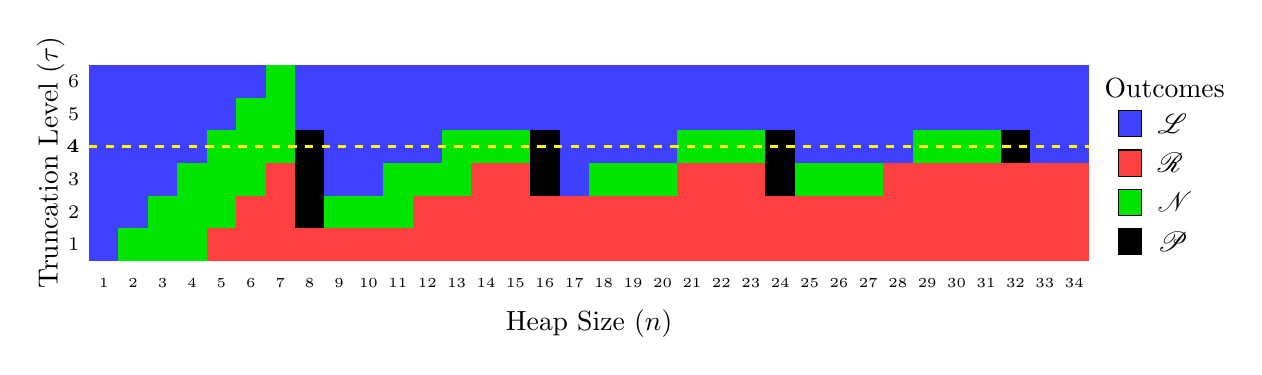
\begin{tikzpicture}[x=0.45cm, y=0.5cm,scale=0.83]
  % Colors
  % \colorlet{cL}{blue!55}
  % \colorlet{cR}{red!55}
  % \colorlet{cN}{gray!15} % Off-white for visibility
  % \colorlet{cP}{black!75}
    \tikzset{fade/.style={fill opacity=1}}
  \colorlet{cL}{blue!75}
  \colorlet{cR}{red!75}
  \colorlet{cN}{green!90!black} % Off-white for visibility
  \colorlet{cP}{black}
  % Colored Blocks
  \fill[cL, fade] (0.5, 0.5) rectangle (1.5, 1.5);
  \fill[cN, fade] (1.5, 0.5) rectangle (2.5, 1.5);
  \fill[cN, fade] (2.5, 0.5) rectangle (3.5, 1.5);
  \fill[cN, fade] (3.5, 0.5) rectangle (4.5, 1.5);
  \fill[cR, fade] (4.5, 0.5) rectangle (5.5, 1.5);
  \fill[cR, fade] (5.5, 0.5) rectangle (6.5, 1.5);
  \fill[cR, fade] (6.5, 0.5) rectangle (7.5, 1.5);
  \fill[cR, fade] (7.5, 0.5) rectangle (8.5, 1.5);
  \fill[cR, fade] (8.5, 0.5) rectangle (9.5, 1.5);
  \fill[cR, fade] (9.5, 0.5) rectangle (10.5, 1.5);
  \fill[cR, fade] (10.5, 0.5) rectangle (11.5, 1.5);
  \fill[cR, fade] (11.5, 0.5) rectangle (12.5, 1.5);
  \fill[cR, fade] (12.5, 0.5) rectangle (13.5, 1.5);
  \fill[cR, fade] (13.5, 0.5) rectangle (14.5, 1.5);
  \fill[cR, fade] (14.5, 0.5) rectangle (15.5, 1.5);
  \fill[cR, fade] (15.5, 0.5) rectangle (16.5, 1.5);
  \fill[cR, fade] (16.5, 0.5) rectangle (17.5, 1.5);
  \fill[cR, fade] (17.5, 0.5) rectangle (18.5, 1.5);
  \fill[cR, fade] (18.5, 0.5) rectangle (19.5, 1.5);
  \fill[cR, fade] (19.5, 0.5) rectangle (20.5, 1.5);
  \fill[cR, fade] (20.5, 0.5) rectangle (21.5, 1.5);
  \fill[cR, fade] (21.5, 0.5) rectangle (22.5, 1.5);
  \fill[cR, fade] (22.5, 0.5) rectangle (23.5, 1.5);
  \fill[cR, fade] (23.5, 0.5) rectangle (24.5, 1.5);
  \fill[cR, fade] (24.5, 0.5) rectangle (25.5, 1.5);
  \fill[cR, fade] (25.5, 0.5) rectangle (26.5, 1.5);
  \fill[cR, fade] (26.5, 0.5) rectangle (27.5, 1.5);
  \fill[cR, fade] (27.5, 0.5) rectangle (28.5, 1.5);
  \fill[cR, fade] (28.5, 0.5) rectangle (29.5, 1.5);
  \fill[cR, fade] (29.5, 0.5) rectangle (30.5, 1.5);
  \fill[cR, fade] (30.5, 0.5) rectangle (31.5, 1.5);
  \fill[cR, fade] (31.5, 0.5) rectangle (32.5, 1.5);
  \fill[cR, fade] (32.5, 0.5) rectangle (33.5, 1.5);
  \fill[cR, fade] (33.5, 0.5) rectangle (34.5, 1.5);
  \fill[cL, fade] (0.5, 1.5) rectangle (1.5, 2.5);
  \fill[cL, fade] (1.5, 1.5) rectangle (2.5, 2.5);
  \fill[cN, fade] (2.5, 1.5) rectangle (3.5, 2.5);
  \fill[cN, fade] (3.5, 1.5) rectangle (4.5, 2.5);
  \fill[cN, fade] (4.5, 1.5) rectangle (5.5, 2.5);
  \fill[cR, fade] (5.5, 1.5) rectangle (6.5, 2.5);
  \fill[cR, fade] (6.5, 1.5) rectangle (7.5, 2.5);
  \fill[cP, fade] (7.5, 1.5) rectangle (8.5, 2.5);
  \fill[cN, fade] (8.5, 1.5) rectangle (9.5, 2.5);
  \fill[cN, fade] (9.5, 1.5) rectangle (10.5, 2.5);
  \fill[cN, fade] (10.5, 1.5) rectangle (11.5, 2.5);
  \fill[cR, fade] (11.5, 1.5) rectangle (12.5, 2.5);
  \fill[cR, fade] (12.5, 1.5) rectangle (13.5, 2.5);
  \fill[cR, fade] (13.5, 1.5) rectangle (14.5, 2.5);
  \fill[cR, fade] (14.5, 1.5) rectangle (15.5, 2.5);
  \fill[cR, fade] (15.5, 1.5) rectangle (16.5, 2.5);
  \fill[cR, fade] (16.5, 1.5) rectangle (17.5, 2.5);
  \fill[cR, fade] (17.5, 1.5) rectangle (18.5, 2.5);
  \fill[cR, fade] (18.5, 1.5) rectangle (19.5, 2.5);
  \fill[cR, fade] (19.5, 1.5) rectangle (20.5, 2.5);
  \fill[cR, fade] (20.5, 1.5) rectangle (21.5, 2.5);
  \fill[cR, fade] (21.5, 1.5) rectangle (22.5, 2.5);
  \fill[cR, fade] (22.5, 1.5) rectangle (23.5, 2.5);
  \fill[cR, fade] (23.5, 1.5) rectangle (24.5, 2.5);
  \fill[cR, fade] (24.5, 1.5) rectangle (25.5, 2.5);
  \fill[cR, fade] (25.5, 1.5) rectangle (26.5, 2.5);
  \fill[cR, fade] (26.5, 1.5) rectangle (27.5, 2.5);
  \fill[cR, fade] (27.5, 1.5) rectangle (28.5, 2.5);
  \fill[cR, fade] (28.5, 1.5) rectangle (29.5, 2.5);
  \fill[cR, fade] (29.5, 1.5) rectangle (30.5, 2.5);
  \fill[cR, fade] (30.5, 1.5) rectangle (31.5, 2.5);
  \fill[cR, fade] (31.5, 1.5) rectangle (32.5, 2.5);
  \fill[cR, fade] (32.5, 1.5) rectangle (33.5, 2.5);
  \fill[cR, fade] (33.5, 1.5) rectangle (34.5, 2.5);
  \fill[cL, fade] (0.5, 2.5) rectangle (1.5, 3.5);
  \fill[cL, fade] (1.5, 2.5) rectangle (2.5, 3.5);
  \fill[cL, fade] (2.5, 2.5) rectangle (3.5, 3.5);
  \fill[cN, fade] (3.5, 2.5) rectangle (4.5, 3.5);
  \fill[cN, fade] (4.5, 2.5) rectangle (5.5, 3.5);
  \fill[cN, fade] (5.5, 2.5) rectangle (6.5, 3.5);
  \fill[cR, fade] (6.5, 2.5) rectangle (7.5, 3.5);
  \fill[cP, fade] (7.5, 2.5) rectangle (8.5, 3.5);
  \fill[cL, fade] (8.5, 2.5) rectangle (9.5, 3.5);
  \fill[cL, fade] (9.5, 2.5) rectangle (10.5, 3.5);
  \fill[cN, fade] (10.5, 2.5) rectangle (11.5, 3.5);
  \fill[cN, fade] (11.5, 2.5) rectangle (12.5, 3.5);
  \fill[cN, fade] (12.5, 2.5) rectangle (13.5, 3.5);
  \fill[cR, fade] (13.5, 2.5) rectangle (14.5, 3.5);
  \fill[cR, fade] (14.5, 2.5) rectangle (15.5, 3.5);
  \fill[cP, fade] (15.5, 2.5) rectangle (16.5, 3.5);
  \fill[cL, fade] (16.5, 2.5) rectangle (17.5, 3.5);
  \fill[cN, fade] (17.5, 2.5) rectangle (18.5, 3.5);
  \fill[cN, fade] (18.5, 2.5) rectangle (19.5, 3.5);
  \fill[cN, fade] (19.5, 2.5) rectangle (20.5, 3.5);
  \fill[cR, fade] (20.5, 2.5) rectangle (21.5, 3.5);
  \fill[cR, fade] (21.5, 2.5) rectangle (22.5, 3.5);
  \fill[cR, fade] (22.5, 2.5) rectangle (23.5, 3.5);
  \fill[cP, fade] (23.5, 2.5) rectangle (24.5, 3.5);
  \fill[cN, fade] (24.5, 2.5) rectangle (25.5, 3.5);
  \fill[cN, fade] (25.5, 2.5) rectangle (26.5, 3.5);
  \fill[cN, fade] (26.5, 2.5) rectangle (27.5, 3.5);
  \fill[cR, fade] (27.5, 2.5) rectangle (28.5, 3.5);
  \fill[cR, fade] (28.5, 2.5) rectangle (29.5, 3.5);
  \fill[cR, fade] (29.5, 2.5) rectangle (30.5, 3.5);
  \fill[cR, fade] (30.5, 2.5) rectangle (31.5, 3.5);
  \fill[cR, fade] (31.5, 2.5) rectangle (32.5, 3.5);
  \fill[cR, fade] (32.5, 2.5) rectangle (33.5, 3.5);
  \fill[cR, fade] (33.5, 2.5) rectangle (34.5, 3.5);
  \fill[cL] (0.5, 3.5) rectangle (1.5, 4.5);
  \fill[cL] (1.5, 3.5) rectangle (2.5, 4.5);
  \fill[cL] (2.5, 3.5) rectangle (3.5, 4.5);
  \fill[cL] (3.5, 3.5) rectangle (4.5, 4.5);
  \fill[cN] (4.5, 3.5) rectangle (5.5, 4.5);
  \fill[cN] (5.5, 3.5) rectangle (6.5, 4.5);
  \fill[cN] (6.5, 3.5) rectangle (7.5, 4.5);
  \fill[cP] (7.5, 3.5) rectangle (8.5, 4.5);
  \fill[cL] (8.5, 3.5) rectangle (9.5, 4.5);
  \fill[cL] (9.5, 3.5) rectangle (10.5, 4.5);
  \fill[cL] (10.5, 3.5) rectangle (11.5, 4.5);
  \fill[cL] (11.5, 3.5) rectangle (12.5, 4.5);
  \fill[cN] (12.5, 3.5) rectangle (13.5, 4.5);
  \fill[cN] (13.5, 3.5) rectangle (14.5, 4.5);
  \fill[cN] (14.5, 3.5) rectangle (15.5, 4.5);
  \fill[cP] (15.5, 3.5) rectangle (16.5, 4.5);
  \fill[cL] (16.5, 3.5) rectangle (17.5, 4.5);
  \fill[cL] (17.5, 3.5) rectangle (18.5, 4.5);
  \fill[cL] (18.5, 3.5) rectangle (19.5, 4.5);
  \fill[cL] (19.5, 3.5) rectangle (20.5, 4.5);
  \fill[cN] (20.5, 3.5) rectangle (21.5, 4.5);
  \fill[cN] (21.5, 3.5) rectangle (22.5, 4.5);
  \fill[cN] (22.5, 3.5) rectangle (23.5, 4.5);
  \fill[cP] (23.5, 3.5) rectangle (24.5, 4.5);
  \fill[cL] (24.5, 3.5) rectangle (25.5, 4.5);
  \fill[cL] (25.5, 3.5) rectangle (26.5, 4.5);
  \fill[cL] (26.5, 3.5) rectangle (27.5, 4.5);
  \fill[cL] (27.5, 3.5) rectangle (28.5, 4.5);
  \fill[cN] (28.5, 3.5) rectangle (29.5, 4.5);
  \fill[cN] (29.5, 3.5) rectangle (30.5, 4.5);
  \fill[cN] (30.5, 3.5) rectangle (31.5, 4.5);
  \fill[cP] (31.5, 3.5) rectangle (32.5, 4.5);
  \fill[cL] (32.5, 3.5) rectangle (33.5, 4.5);
  \fill[cL] (33.5, 3.5) rectangle (34.5, 4.5);
  \fill[cL, fade] (0.5, 4.5) rectangle (1.5, 5.5);
  \fill[cL, fade] (1.5, 4.5) rectangle (2.5, 5.5);
  \fill[cL, fade] (2.5, 4.5) rectangle (3.5, 5.5);
  \fill[cL, fade] (3.5, 4.5) rectangle (4.5, 5.5);
  \fill[cL, fade] (4.5, 4.5) rectangle (5.5, 5.5);
  \fill[cN, fade] (5.5, 4.5) rectangle (6.5, 5.5);
  \fill[cN, fade] (6.5, 4.5) rectangle (7.5, 5.5);
  \fill[cL, fade] (7.5, 4.5) rectangle (8.5, 5.5);
  \fill[cL, fade] (8.5, 4.5) rectangle (9.5, 5.5);
  \fill[cL, fade] (9.5, 4.5) rectangle (10.5, 5.5);
  \fill[cL, fade] (10.5, 4.5) rectangle (11.5, 5.5);
  \fill[cL, fade] (11.5, 4.5) rectangle (12.5, 5.5);
  \fill[cL, fade] (12.5, 4.5) rectangle (13.5, 5.5);
  \fill[cL, fade] (13.5, 4.5) rectangle (14.5, 5.5);
  \fill[cL, fade] (14.5, 4.5) rectangle (15.5, 5.5);
  \fill[cL, fade] (15.5, 4.5) rectangle (16.5, 5.5);
  \fill[cL, fade] (16.5, 4.5) rectangle (17.5, 5.5);
  \fill[cL, fade] (17.5, 4.5) rectangle (18.5, 5.5);
  \fill[cL, fade] (18.5, 4.5) rectangle (19.5, 5.5);
  \fill[cL, fade] (19.5, 4.5) rectangle (20.5, 5.5);
  \fill[cL, fade] (20.5, 4.5) rectangle (21.5, 5.5);
  \fill[cL, fade] (21.5, 4.5) rectangle (22.5, 5.5);
  \fill[cL, fade] (22.5, 4.5) rectangle (23.5, 5.5);
  \fill[cL, fade] (23.5, 4.5) rectangle (24.5, 5.5);
  \fill[cL, fade] (24.5, 4.5) rectangle (25.5, 5.5);
  \fill[cL, fade] (25.5, 4.5) rectangle (26.5, 5.5);
  \fill[cL, fade] (26.5, 4.5) rectangle (27.5, 5.5);
  \fill[cL, fade] (27.5, 4.5) rectangle (28.5, 5.5);
  \fill[cL, fade] (28.5, 4.5) rectangle (29.5, 5.5);
  \fill[cL, fade] (29.5, 4.5) rectangle (30.5, 5.5);
  \fill[cL, fade] (30.5, 4.5) rectangle (31.5, 5.5);
  \fill[cL, fade] (31.5, 4.5) rectangle (32.5, 5.5);
  \fill[cL, fade] (32.5, 4.5) rectangle (33.5, 5.5);
  \fill[cL, fade] (33.5, 4.5) rectangle (34.5, 5.5);
  \fill[cL, fade] (0.5, 5.5) rectangle (1.5, 6.5);
  \fill[cL, fade] (1.5, 5.5) rectangle (2.5, 6.5);
  \fill[cL, fade] (2.5, 5.5) rectangle (3.5, 6.5);
  \fill[cL, fade] (3.5, 5.5) rectangle (4.5, 6.5);
  \fill[cL, fade] (4.5, 5.5) rectangle (5.5, 6.5);
  \fill[cL, fade] (5.5, 5.5) rectangle (6.5, 6.5);
  \fill[cN, fade] (6.5, 5.5) rectangle (7.5, 6.5);
  \fill[cL, fade] (7.5, 5.5) rectangle (8.5, 6.5);
  \fill[cL, fade] (8.5, 5.5) rectangle (9.5, 6.5);
  \fill[cL, fade] (9.5, 5.5) rectangle (10.5, 6.5);
  \fill[cL, fade] (10.5, 5.5) rectangle (11.5, 6.5);
  \fill[cL, fade] (11.5, 5.5) rectangle (12.5, 6.5);
  \fill[cL, fade] (12.5, 5.5) rectangle (13.5, 6.5);
  \fill[cL, fade] (13.5, 5.5) rectangle (14.5, 6.5);
  \fill[cL, fade] (14.5, 5.5) rectangle (15.5, 6.5);
  \fill[cL, fade] (15.5, 5.5) rectangle (16.5, 6.5);
  \fill[cL, fade] (16.5, 5.5) rectangle (17.5, 6.5);
  \fill[cL, fade] (17.5, 5.5) rectangle (18.5, 6.5);
  \fill[cL, fade] (18.5, 5.5) rectangle (19.5, 6.5);
  \fill[cL, fade] (19.5, 5.5) rectangle (20.5, 6.5);
  \fill[cL, fade] (20.5, 5.5) rectangle (21.5, 6.5);
  \fill[cL, fade] (21.5, 5.5) rectangle (22.5, 6.5);
  \fill[cL, fade] (22.5, 5.5) rectangle (23.5, 6.5);
  \fill[cL, fade] (23.5, 5.5) rectangle (24.5, 6.5);
  \fill[cL, fade] (24.5, 5.5) rectangle (25.5, 6.5);
  \fill[cL, fade] (25.5, 5.5) rectangle (26.5, 6.5);
  \fill[cL, fade] (26.5, 5.5) rectangle (27.5, 6.5);
  \fill[cL, fade] (27.5, 5.5) rectangle (28.5, 6.5);
  \fill[cL, fade] (28.5, 5.5) rectangle (29.5, 6.5);
  \fill[cL, fade] (29.5, 5.5) rectangle (30.5, 6.5);
  \fill[cL, fade] (30.5, 5.5) rectangle (31.5, 6.5);
  \fill[cL, fade] (31.5, 5.5) rectangle (32.5, 6.5);
  \fill[cL, fade] (32.5, 5.5) rectangle (33.5, 6.5);
  \fill[cL, fade] (33.5, 5.5) rectangle (34.5, 6.5);
  
  % Grid Lines
  % \draw[step=1.0, black, thin] (0.5, 0.5) grid (34.5, 6.5);
  \draw[yellow!90,dashed, line width=1pt]
    (0.5,4) -- (34.5,4);
  % Axes Ticks
  \foreach \n in {1, 2, ..., 34} \node[below, font=\tiny] at (\n, 0.25) {\n};
  \foreach \k in {1,2,3,4,5,6}{
    \ifnum\k=4
        \node[left,font=\scriptsize] at (0.5,\k) {\textbf{\k}};
    \else
        \node[left,font=\scriptsize] at (0.5,\k) {\k};
    \fi
}
  % Axes Labels
  \node[below=0.5cm] at (17.5, 0.5) {Heap Size ($n$)};
  \node[rotate=90, above=1cm] at (0, 1.1) {Truncation Level ($\tau$)};

  % Highlight row k=4
  % \draw[line width=2pt, orange] (0.5, 3.5) rectangle (34.5, 4.5);

%   \draw[yellow!90, line width=1pt]
%     (0.5,3.5) -- (34.5,3.5);

% \draw[yellow!90, line width=1pt]
%     (0.5,4.5) -- (34.5,4.5);

  % Legend
  \begin{scope}[shift={(35.5, 3.5)}]
    \node[right] at (-0.8, 2.3) {Outcomes};
    \draw[fill=cL, fade] (0, 0.8) rectangle (0.8, 1.6); \node[right] at (1, 1.2) {$\mathscr{L}$};
    \draw[fill=cR, fade] (0, -0.4) rectangle (0.8, 0.4); \node[right] at (1, 0) {$\mathscr{R}$};
    \draw[fill=cN, fade] (0, -1.6) rectangle (0.8, -0.8); \node[right] at (1, -1.2) {$\mathscr{N}$};
    \draw[fill=cP, fade] (0, -2.8) rectangle (0.8, -2.0); \node[right] at (1, -2.4) {$\mathscr{P}$};
  \end{scope}
\end{tikzpicture}
\caption{Outcomes of $\ts_\tau(n; 3, 7)$. Blue, red, green, and black cells represent $\mathscr{L}$, $\mathscr{R}$, $\mathscr{N}$, and $\mathscr{P}$ outcomes, respectively. The row corresponding to the truncation level at which $\pp$- and $\np$-positions occur infinitely often is highlighted.}
\label{fig: outcomes of ts(n,3,7)}
\end{figure}


For fixed $a,b$ and $\tau$, we say that the ruleset
$\ts_\tau(n;a,b)$ is \emph{Right-dominating} if $\ts_\tau(n;a,b)\in \rp$, for all sufficiently large $n$. Similarly, if $\ts_\tau(n;a,b)\in \lp$ for all sufficiently large $n$, we say that the ruleset is \emph{Left-dominating}. If the ruleset is neither Left- nor Right-dominating, we call it \emph{balanced}.


This motivates the following questions: does the ruleset progress systematically from being Right-dominating at small truncation levels, to balanced in the middle, and finally Left-dominating at large truncation levels? If this is the case, what is the minimum truncation level at which the ruleset first becomes balanced? We refer to this specific truncation level as the \emph{critical threshold}. This naturally leads to another interesting question: is the ruleset balanced exclusively at the critical threshold, or does this balanced behavior occur across multiple truncation levels?
% Figure~\ref{fig: outcomes of ts(n,3,7)} and other experiments suggest that given $a$ and $b$, {\sc Truncated Support} is Right-dominating for all truncation levels below $b-a$, balanced at the truncation level $b-a$ and Left-dominating for all truncation levels above $b-a$. We prove it in our third main result.
In line with these questions, Figure~\ref{fig: outcomes of ts(n,3,7)} and many other experiments had suggested to us that, for fixed $a$ and $b$, {\sc Truncated Support} is Right-dominating for truncation levels below $b-a$, balanced at truncation level $b-a$, and Left-dominating for truncation levels above $b-a$. Our third main result establishes this trichotomy.

\begin{theorem}[Outcomes of TS]\label{thm: outcomes of TS}
    Consider $G=\ts_\tau(n;a,b)$ where $a<b$. 
    \begin{enumerate}
        \item\label{item:thm: outcomes of TS:1} If $\tau>b-a$, then $G\in \lp$, for all $n\ge b+1$.
        % \item If $\tau>b-a$, then, for all $n\ge b+1$, $G\in \lp$.
        \item\label{item:thm: outcomes of TS:2} If $\tau=b-a$, let $t = n\bmod (b+1)$, $0\le t\le b$. Then, for all $n\ge 0$,
        \begin{enumerate}
            \item $G\in \pp$, if $t=0$;  
            \item $G\in \lp$, if $1\le t\le \tau$;
            \item $G\in \np$, if $\tau+1\le t\le b$. 
            \end{enumerate}
        \item\label{item:thm: outcomes of TS:3} If $\tau<b-a$, then $G\in \rp$, for all $n\ge \left\lfloor\frac{b-a}{b-a-\tau}\right\rfloor\!(a+\tau+1)$.
        \end{enumerate}
\end{theorem}


Theorem~\ref{thm: outcomes of TS} proves that $b-a$ is the critical threshold. Below this threshold the ruleset is Right-dominating, and above it, the ruleset is Left-dominating. Therefore, we call the level $\kappa:=b-a$ the {\em knife's edge}. 

The second part of Theorem~\ref{thm: outcomes of TS} says that the outcome of {\sc TS} at the knife's edge is periodic with period $b+1$. Tables~\ref{tab:CF of ts_4(n,3,7)} and \ref{tab: cf of ts1(n;5,6)} suggest an even stronger phenomenon: not only is the outcome periodic, but the canonical forms of {\sc TS} at the knife's edge is also periodic with the same period length. Our next theorem establishes this periodicity of the canonical forms.% at the knife's edge. 

% The third item of this theorem shows that the outcome of {\sc TS} at truncation level $b-a$ is periodic with period $b+1$. Tables~\ref{tab:CF of ts_4(n,3,7)} and \ref{tab: cf of ts1(n;5,6)} suggest an even stronger phenomenon: not only the outcomes, but also the canonical forms are periodic with the same period. The next theorem establishes this periodicity of the canonical forms.

\begin{table}[h!]
    \centering
    \caption{Canonical forms of $\ts_{4}(n;3,7)$ for $0 \le n \le 15$.}
    \label{tab:CF of ts_4(n,3,7)}
    
    \setlength{\tabcolsep}{4pt}
    \renewcommand{\arraystretch}{1.2}
    
    % ---------- First table ----------
    \begin{minipage}{0.48\textwidth}
    \centering
    \small
    \begin{tabular}{|l|c|}
    \hline
    $n$ & $G$ \\ \hline
    0  & 0 \\ \hline
    1  & 1 \\ \hline
    2  & 2 \\ \hline
    3  & 3 \\ \hline
    4  & 4 \\ \hline
    5  & $\{4|0\}$ \\ \hline
    6  & $\{4, \{4|0\} | 0\}$ \\ \hline
    7  & $\{4, \{4, \{4|0\} | 0\} | 0\}$ \\ \hline
    
    \end{tabular}
    \end{minipage}
    \hfill
    % ---------- Second table ----------
    \begin{minipage}{0.48\textwidth}
    \centering
    \small
    \begin{tabular}{|l|c|}
    \hline
    $n$ & $G$ \\ \hline
    8  & 0 \\ \hline
    9  & 1 \\ \hline
    10 & 2 \\ \hline
    11 & 3 \\ \hline
    12 & 4 \\ \hline
    13 & $\{4|0\}$ \\ \hline
    14 & $\{4, \{4|0\} | 0\}$ \\ \hline
    15 & $\{4, \{4, \{4|0\} | 0\} | 0\}$ \\ \hline
    % 16 & 0 \\ \hline
    % 17 & 1 \\ \hline
    % 18 & 2 \\ \hline
    % 19 & 3 \\ \hline
    % 20 & 4 \\ \hline
    % 21 & $\{4|0\}$ \\ \hline
    % 22 & $\{4, \{4|0\} | 0\}$ \\ \hline
    % 23 & $\{4, \{4, \{4|0\} | 0\} | 0\}$ \\ \hline
    % 24 & 0 \\ \hline
    % 25 & 1 \\ \hline
    % 26 & 2 \\ \hline
    \end{tabular}
    \end{minipage}
\end{table}
%\begin{theorem}\label{thm: CF periodicity in TS at b-a}
%    For fixed positive integers $a$ and $b$ such that $a<b$, let $G=\ts_{b-a}(n;a,b)$ be an instance of {\sc Truncated Support}. Then $G=\ts_{b-a}(r;a,b)$ where $r=n \bmod (b+1)$.
%\end{theorem}

\begin{theorem}[Canonical Form Periodicity in TS]\label{thm: CF periodicity in TS at b-a}
    Fix $a,b$ and let $\kappa =b-a$. Let $G\coloneq\ts_{\kappa}(n;a,b)$ where $a<b$. Let $t= n \bmod (b+1)$, with $0\le t\le b$. Then $G=\ts_{\kappa}(t;a,b)$. %Consider $G=\ts_{b-a}(n;a,b)$ where $a<b$. Let $t$ be the remainder when $n$ is divided by $b+1$. Then $G=\ts_{b-a}(t;a,b)$.
    % Let $a$ and $b$ be positive integers such that $a<b$. Then 
    % \begin{align}\label{eq:PTS}
    %         \ts_{b-a}(n;a,b)=\ts_{b-a}(m;a,b),
    % \end{align}
    % if $m=n (mod\; b+1)$.
\end{theorem}

% Atomic weight can be helpful when playing disjunctive sums of games. Intuitively, the atomic weight of a game component measures the number of moves a player can delay playing there before the opponent can terminate this component. In that sense, it is an analogue to `numbers' in the atomic world of games. 
Recall when playing disjunctive sums of games, information about outcome alone (Theorem~\ref{thm: outcomes of TS}) is often insufficient. And often canonical forms are not accessible. Still one needs additional information; then atomic weight comes to play.
% \footnote{If the game is an infinitesimal, atomic weight is useful when analyzing disjunctive sums. For hot games, temperature may be more informative, while for numbers the canonical form alone suffices.}

Table~\ref{tab:aw of ts(n,3,7)} suggests a clear pattern in the atomic weights of $\ts_\tau(n;3,7)$. For $\tau<b-a$, the pattern begins exactly at heap size
$n'=\left\lfloor\frac{b-a}{b-a-\tau}\right\rfloor\!(a+\tau+1)$. By Theorem~\ref{thm: outcomes of TS}, starting from $n'$, all larger heap sizes have outcome $\rp$. If a heap size is larger than or equal to $n'$, Right can postpone making a move until Left is able to reduce the heap below $n'$. Since Left removes at most $a$ tokens per move, she needs at least
\[
\left\lceil\frac{n-(n'-1)}{a}\right\rceil
\]
to reduced the heap below $n'$. Thus, Right can delay his move for exactly $\left\lceil\frac{n-(n'-1)}{a}\right\rceil-1$ many turns, suggesting that the atomic weight is
\[
\left\lceil\frac{n-n'+1}{a}\right\rceil-1=\left\lfloor\frac{n-n'}{a}\right\rfloor.
\] 

Our fourth main result proves this formula for all $\tau<(b-a)/2$. Furthermore, we conjecture that the formula remains valid for $(b-a)/2\le\tau<b-a$. Note that {\sc TS} games are not all-small: if $\tau>0$ then a heap of size one has value $1$. Thus, atomic weights  do not exist for all possible heap sizes. However, it turns out that many {\sc TS} games are atomic, and have atomic weight. 

% To play in disjunctive sum of games, the information about outcomes is not enough, atomic weight of the games is also required.\footnote{If the game is an infinitesimal, atomic weight is helpful when playing in disjunctive sum of games, but in case of a hot game, temperature might be useful, and if the game is a number, the canonical form is enough}.  Table~\ref{tab:aw of ts(n,3,7)} shows the atomic weight of $\ts_\tau(n;3,7)$. Given $a,b$ and $\tau$, if $\tau<b-a$, we see that the atomic weight shows a clear pattern starting from heap size $R_{\hbeta}=\hbeta(a+\tau+1)$, exactly the heap size starting from where all further positions are $\rp$. If $n>R_{\hbeta}$, then Right can delay his move as long as Left cannot reach a heap size below $R_{\hbeta}$, as starting from $R_{\hbeta}$, all heap sizes have outcome $\rp$. Since, Left can at most remove $a$ tokens in one move, she requires at least $\lfloor(n-R_{\hbeta})/a\rfloor$ to reach a heap size from where she can move to a heap size below $R_{\hbeta}$ in one move. This means Right can delay his move for $\lfloor(n-R_{\hbeta})/a\rfloor$ many moves, before Left gets a chance to win, hence the atomic weight should be $\lfloor(n-R_{\hbeta})/a\rfloor$. We prove this formula of atomic weight for all $\tau<(b-a)/2$ and leave it as a conjecture for $(b-a)/2\le \tau<b-a$. 

% she cannot reach a heap size below $R_{\hbeta}$ in  ach Starting from $R_{\hbeta}$, the first $a$ heap sizes have $0$ atomic weight, the next $a$ heap sizes have $-1$ atomic weight, and the next $a$ heap sizes have $-2$ atomic weight and so on. 

% As seen in {\sc Full Support}, the information about outcomes is not enough to play strategically in disjunctive sum of games. For this purpose, we must compute the atomic weight.  compute the atomic weight of {\sc TS} for all large $n$ for truncation levels $\tau<(b-a)/2$ in out next main result. 

\begin{theorem}[Atomic Weight of {\sc TS}]\label{thm: AW of TS}
    Let $a,b$ and $\tau$ are positive integers such that $a<b$. If $1\le \tau< (b-a)/2$, then for all $n\ge a+\tau+1$, 
    \begin{align}\label{eq:w}
    \aw\big(\ts_\tau(n;a,b)\big)=-\left\lfloor \frac{n-(a+\tau+1)}{a}\right\rfloor.
    \end{align}
\end{theorem}

% We also conjecture the formula for atomic weight of {\sc TS} for $(b-a)/2\le \tau<b-a$ in Conjecture~\ref{con: AW of TS for all k<b-a}. 

% For complete information about the outcomes, we find the first $b+1$ outcomes of {\sc TS} ruleset at  truncation level $b-a$ in Lemma~\ref{lem: outcome ts at b-a}.




% While playing Full and Truncated support games in disjunctive sum, the knowledge of outcomes of individual components is not enough to determine the outcome of the overall game. So, we next compute the atomic weight of {\sc TS} for large heap sizes at truncation levels below $(b-a)/2$. Note that not all {\sc TS} positions have atomic weight, and furthermore, some of {\sc TS} positions are not even infinitesimal.  




% Table~\ref{tab:aw of ts(n,3,7)} shows the pattern of atomic weights of $\ts_\tau(n;3,7)$ for different $n$ and $k$. 

\begin{table}[t!]
\centering
\caption{Atomic weights of $\ts_\tau(n;3,7)$ for $1 \le n \le 34$ and truncation levels $\tau\le 4$. A cell is colored red, if the cell and all the cells below it are $\rp$-positions.}
\label{tab:aw of ts(n,3,7)}

\setlength{\tabcolsep}{4pt}
\renewcommand{\arraystretch}{1.2}

% ---------- First table ----------
\begin{minipage}{0.49\textwidth}
\centering
\small
\begin{tabular}{|l|*{6}{c|}}
\hline
\textbf{$n \backslash \tau$} & 1 & 2 & 3 & 4  \\ \hline
1 &      &      &      &           \\ \hline
 2 &      &      &      &         \\ \hline
 3 &      &      &      &          \\ \hline
 4 &      &      &      &           \\ \hline
 5 & \cellcolor{red!25}0    &      &      &           \\ \hline
 6 & \cellcolor{red!25}0    & 0    &      &          \\ \hline
 7 & \cellcolor{red!25}0   & 0    & 0    &          \\ \hline
 8 & \cellcolor{red!25}-1   & 0    & 0    & 0       \\ \hline
 9 & \cellcolor{red!25}-1   & 0    &      &           \\ \hline
 10 &\cellcolor{red!25} -1   & 1    &      &        \\ \hline
11 & \cellcolor{red!25}-2   & 1    &      &           \\ \hline
12 & \cellcolor{red!25}-2   & \cellcolor{red!25}0    &      &         \\ \hline
13 & \cellcolor{red!25}-2   & \cellcolor{red!25}0    &      &          \\ \hline
14 & \cellcolor{red!25}-3   & \cellcolor{red!25}0    & 0    &          \\ \hline
15 & \cellcolor{red!25}-3   & \cellcolor{red!25}-1   & 0    &           \\ \hline
16 & \cellcolor{red!25}\;-3 \;  &\; \cellcolor{red!25}-1\;   &\; 0\;    &\; 0\;         \\ \hline
17 & \cellcolor{red!25}-4   & \cellcolor{red!25}-1   &      &           \\ \hline
\end{tabular}
\end{minipage}
\hfill
% ---------- Second table ----------
\begin{minipage}{0.49\textwidth}
\centering
\small
\begin{tabular}{|l|*{6}{c|}}
\hline
\textbf{$n \backslash \tau$} & 1 & 2 & 3 & 4 \\ \hline
18 & \cellcolor{red!25}-4   &\cellcolor{red!25} -2   &      &            \\ \hline
19 & \cellcolor{red!25}-4   & \cellcolor{red!25}-2   &      &          \\ \hline 
20 & \cellcolor{red!25}-5   &\cellcolor{red!25} -2   &      &           \\ \hline
21 & \cellcolor{red!25}-5   &\cellcolor{red!25} -3   & 0    &          \\ \hline
22 &\cellcolor{red!25} -5   & \cellcolor{red!25}-3   & 0    &            \\ \hline
23 & \cellcolor{red!25}-6   & \cellcolor{red!25}-3   & 0    &           \\ \hline
24 &\cellcolor{red!25}-6   &\cellcolor{red!25}-4   & 0    & 0         \\ \hline
25 &\cellcolor{red!25} -6   & \cellcolor{red!25}-4   & 0    &           \\ \hline
26 &\cellcolor{red!25} -7   & \cellcolor{red!25}-4   & 1    &           \\ \hline
27 &\cellcolor{red!25} -7   & \cellcolor{red!25}-5   & 1    &            \\ \hline
28 &\cellcolor{red!25} -7   & \cellcolor{red!25}-5   &\cellcolor{red!25} 0    &            \\ \hline
29 &\cellcolor{red!25} -8   & \cellcolor{red!25}-5   &\cellcolor{red!25} 0    &            \\ \hline
30 &\cellcolor{red!25} -8   & \cellcolor{red!25}-6   &\cellcolor{red!25} 0    &            \\ \hline
31 & \cellcolor{red!25}-8   &\cellcolor{red!25} -6   & \cellcolor{red!25}-1   &            \\ \hline
32 & \;\cellcolor{red!25}-9\;   & \cellcolor{red!25}\;-6\;   & \cellcolor{red!25}\;-1\;   & \;0 \;         \\ \hline
33 & \cellcolor{red!25}-9   &\cellcolor{red!25} -7   & \cellcolor{red!25}-1   &            \\ \hline
34 & \cellcolor{red!25}-9   &\cellcolor{red!25} -7   & \cellcolor{red!25}-2   &           \\ \hline
\end{tabular}
\end{minipage}
\end{table}


% Theorems~\ref{thm: CF periodicity in TS at b-a} and \ref{thm: AW of TS} partially prove the fact that the critical threshold is $b-a$ and the ruleset is balanced exclusively at this truncation level. But we leave it as an open problem to prove this fact fully, i.e, to prove that the ruleset is Right-dominating for all $(b-a)/2\le k<b-a$.

% We strongly believe that the critical threshold is $b-a$, and consequently, the ruleset is balanced exclusively at this truncation level. It is partially proved
The rest of the paper is organized as follows:\begin{enumerate}
    \item In Section~\ref{sec: literature review}, we cite the relevant papers and the papers that inspired this work.
    \item In Section~\ref{sec: CF of FS}, we prove our first main result, Theorem~\ref{thm: CF of FS}, about the canonical form of {\sc Full Support}.
    \item In Section~\ref{sec: AW of FS}, we compute the atomic weight of {\sc FS} proving our second main result, Theorem~\ref{thm: aw of FS}.
    \item In Section~\ref{sec: TS}, we introduce {\sc Truncated Support} and prove our third main result, Theorem~\ref{thm: outcomes of TS}, part-wise in subsections~\ref{subsec: higher truncation level}, \ref{subsec: balanced truncation level} and \ref{subsec: lower truncation level}. Along with this, we also prove Theorem~\ref{thm: CF periodicity in TS at b-a}, which says that the canonical form of {\sc TS} is periodic at the knife's edge.
    
    % \item In Section~\ref{sec: TS}, we introduce {\sc Truncated Support} and prove our third main result part-wise in subsections~\ref{subsec: higher truncation level}, \ref{subsec: balanced truncation level} and \ref{subsec: lower truncation level}, Theorem~\ref{thm: outcomes of TS}, about the outcomes of {\sc TS}. Along with this, we also prove Theorem~\ref{thm: CF periodicity in TS at b-a}, which says that the canonical form of {\sc TS} is periodic at the knife's edge.
    \item In Section~\ref{sec: AW of TS}, we prove our fourth main result, Theorem~\ref{thm: AW of TS}, which gives a partial formula for the atomic weights of {\sc TS}. 
\end{enumerate}

% We believe that the truncation level at which the game is balanced is unique, but this remains an open problem.



% Since the canonical form of {\sc TS} shows a periodic behavior at the truncation level $b-a$ with period length $b+1$, we try to study these $b+1$ canonical forms. Tables~\ref{tab:CF of ts_4(n,3,7)} and \ref{tab: cf of ts1(n;5,6)} show the canonical forms of two different {\sc TS} rulesets at their corresponding critical thresholds. We find many dominated options in these games proved that the number of dominated options is directly proportional to $b-a$ and also find those options in Proposition~\ref{prop: domination at b-a}.


% \an{Furthermore, we show that many options in the canonical form of {\sc TS} at the critical threshold are dominated unless $b-a$ is very small in Proposition~\ref{prop: domination at b-a}.}



\section{Literature review}\label{sec: literature review}

{\sc Impartial Subtraction} games have been extensively studied and are well known for exhibiting periodic outcome sequences. In contrast, {\sc Partizan Subtraction} games are significantly more complex because the players have different move sets. Their analysis often requires algebraic tools from CGT, such as canonical forms, reduced canonical forms, temperatures, and atomic weights.
% {\sc Impartial Subtraction} games have been extensively studied. They often demonstrate periodic pattern of outcomes. Whereas, {\sc Partizan Subtraction} presents significantly more complexity because the move sets of the two players differ, requiring algebraic tools from CGT such as canonical forms, reduced canonical forms, temperatures and atomic weights.

The study of {\sc Partizan Subtraction} began with the work of Fraenkel and Kotzig \cite{FA} (1987), who introduced partizan octal games. They proved that every partizan subtraction game with finite subtraction sets has an ultimately periodic outcome sequence and introduced the notion of dominance, which we refer to as Left- and Right-domination.

% In 1987, Fraenkel and Kotzig \cite{FA} established the baseline for {\sc Partizan Subtraction} through their study of partizan octal games. They proved that all partizan subtraction games with finite subtraction sets exhibit periodicity in outcomes and introduced the notion of Dominance, which we call Left- and Right-domination. Almost 20 years later, the Mesdal group \cite{M} analyzed partizan subtraction rulesets with finite subtraction sets using reduced canonical forms. 

Mesdal et al.~\cite{M} later investigated finite partizan subtraction rulesets, where players may optionally split the heap after removal, through reduced canonical forms, extending the structural understanding of these games beyond their outcomes.

Larsson et al. \cite{LMNS} studied a different class of partizan subtraction games in which the players have complementary infinite subtraction sets generated by the $\pp$-positions of Wythoff Nim and Fibonacci sequences. They prove that every position is either a reduced canonical form switch or a canonical form number.

More recently, Duchêne et al.~\cite{DHNP} analyzed partizan subtraction games with subtraction sets of size two. Besides Left- and Right-domination, they identified three additional asymptotic behaviors of the outcome sequence: weak dominance, fairness, and ultimate impartiality. Weak dominance occurs when the outcome sequence is eventually periodic and the period contains either $\lp$ or $\rp$, but not both. The {\sc TS} ruleset at truncation level $b-a$ studied in this paper exhibits weak dominance, since its periodic outcome sequence contains $\lp$-positions but no $\rp$-positions. They prove NP-hardness of {\sc Partizan Subtraction}, if the ruleset is included in the input, by reduction to the unbounded knapsack problem. 

% The next paper on Partizan Subtraction came in 2018 by Larsson, Mckay, Nowakowski and Siegel \cite{LMNS}. In their model, both players possess complementary infinite subtraction sets determined by Fibonacci sequences, and the authors successfully derived reduced canonical forms. 

% In 2022, Duchêne et. al. \cite{DHNP}, studied partizan subtraction for size two subtraction sets and derived three other behaviors of outcome sequence other than dominance, namely weak dominance, fairness and ultimate impartiality. Weak dominance occurs when the outcome sequence is eventually periodic and the period contains either $\lp$ or $\rp$, but not both. In our paper, Truncated support at truncation level $b-a$ shows the weak dominance behavior as the period contains $\lp$ but not $\rp$.

The {\sc Full Support} ruleset also belongs to the class of cumulative games, introduced by Larsson, Meir, and Zick \cite{URYCG2020}. In cumulative games, player cumulations are part of the rules of how to move; they may contribute to the players payoffs when the game ends. {\sc Wealth Nim} (also called {\sc Wealth Pebbles}) is one such ruleset family. {\sc Full Support} with $S_L=[a]$ and $S_R=[b]$ is equivalent to {\sc Wealth Nim} with players' wealths $a$ and $b$, and where there is no cumulative effect. 
\begin{figure}
    \centering
    \includegraphics[width=0.5\linewidth]{Wealth_Partizan_and_Full_Support.png}
    \caption{{\sc Full Support} lies at the intersection of {\sc Partizan Subtraction} and Cumulative Games.}
    \label{fig:placeholder}
\end{figure}

Another example of a cumulative game is {\sc Robin Hood} \cite{BDL}. %Unlike {\sc Full Support}, where the subtraction sets remain fixed throughout the game, the subtraction sets in {\sc Robin Hood} evolve after every move. 
Similar to {\sc FS}, Players in {\sc Robin Hood} can remove any number of tokens up to their wealth. However, the wealths of the players remain fixed throughout a game in {\sc FS}, whereas, in {\sc Robin Hood}, if a player remove $m$ tokens from the heap, the opponent's wealth decreases by $m$. Therefore, players want to play first in {\sc Robin Hood} and decrease their opponent's wealth. 
%In this instance of {\sc Wealth Nim} the number of removed tokens is also subtracted from the opponents' wealth. 

% Cumulative Games were defined in \cite{URYCG2020}. These games lies at the intersection of classical game theory and combinatorial game theory. The ruleset {\sc Wealth Nim} a.k.a.\ {\sc Wealth Pebbles} is an example of cumulative games. In this ruleset, player cumulations are part of the rules of how to move, but do not contribute to the players gain when the game ends. {\sc Full Support} with $S_L=[a]$ and $S_R=[b]$ is an example of {\sc Wealth Nim} with players' wealth $a$ and $b$. Another example of cumulative games is {\sc Robin Hood} in \cite{BDL}. The difference between {\sc Robin Hood} and {\sc Full Support} is that the subtraction sets changes in the former after every move, whereas it remains the same throughout the game in later. 

% Since the purpose of \cite{URYCG2020} is to provide a broad framework for further study, no efforts were made to solve proposed individual games and rulesets. This research is among the first ones to do so.






% The {\sc FS} ruleset lies at the intersection of partizan subtraction and cumulative games. As noted in the introduction, the {\sc FS} ruleset is equivalent to {\sc Wealth Nim}, where $a$ and $b$ represent the ``wealth" of the players. This links the research to the work of Larsson, Meir, and Zick \cite{URYCG2020} on cumulative games. 

When both players have the same subtraction set, {\sc Full Support} becomes impartial. In this case, the nim-values were determined in \cite{BCG2004}. We restate the formula and include its folklore proof for completeness.

% \begin{theorem}\label{thm: CF of FS for equal wealth}
%     Let $n\in\Nat_0$ and $a\in \Nat$. If $r$ denotes $n \mod (a+1)$. Then, $\fs(n;a,a)=
%         *r$.
% \end{theorem}

\begin{theorem}[Impartial FS]\label{thm: CF of FS for equal wealth}
Let $a\in\Nat_0$. For all  $n\in \Nat$,  let $r=n \bmod (a+1)$. Then $\fs(n;a,a)~=~*r.$
\end{theorem}
\begin{proof}
%By Observation~\ref{obs: fs positions for small n}, for all
%$n\in\{0\}\cup [a]$, we have $\fs(n;a,a)=*n$.

%Now assume that the statement holds for all options of $\fs(n;a,a)$. 
If $n\le a$, the game is {\sc nim}, and otherwise we  have 
\begin{align*}
\fs(n;a,a)
&= \{\fs(n-1;a,a), \fs(n-2;a,a), \dots, \fs(n-a;a,a)\} \\
&=\{*((n-1)\bmod (a+1)),\;*((n-2)\bmod(a+1)),\; \dots,\; *((n-a)\bmod(a+1))\}\\
&= \{*((r-1)\bmod(a+1)), *((r-2)\bmod(a+1)), \dots, *((r-a)\bmod(a+1))\} \\
&= *r.
\end{align*}

The second equality follows by induction, and the third is by the statement. For the final equality, observe that
\[
\{r,\; (r-1)\bmod(a+1),\; (r-2)\bmod(a+1), \dots,\; (r-a)\bmod(a+1)\}
= \{0,1,\dots,a\}.
\]
Hence, $\mathrm{mex}\{(r-1)\bmod(a+1), (r-2)\bmod(a+1), \dots, (r-a)\bmod(a+1)\}=r$.
%which completes the proof.
\end{proof}

We next study the canonical form of {\sc Full Support} when the players have different subtraction sets.

\section{Canonical forms of Full Support}\label{sec: CF of FS}

We assume $a<b$ without loss of generality. 
\begin{definition}[Full Support]
    {\sc Full Support} ({\sc FS}) is a partizan subtraction ruleset played on a single heap, where the subtraction sets of Left and Right are defined by the positive integers $a$ and $b$ with $S_L=[a]$ and $S_R=[b]$. For a heap size $n$, the game is denoted by $\fs(n;a,b)$.
\end{definition}

Symmetrically, in $\fs(n;b,a)$, the subtraction sets are $S_L=[b]$ and $S_R=[a]$.
We start by exploring simple {\sc Full Support} positions.

\begin{observation}\label{obs: fs positions for small n}
    %Let $a,b$ and $n$ be positive integers. 
    Let $G=\fs(n;a,b)$ be an instance of {\sc FS}. Then 
    \begin{enumerate}
        \item $G$ is all-small;
        \item $G=*n$ if $n\le \min(a,b)$.
    \end{enumerate}


%\begin{proof}
    For the first statement, note that both players can remove one pebble whenever $n>0$, so every nonzero position has options for both players and hence, $G$ is all-small. For the second statement, if $n\le \min(a,b)$, then both players may remove any number of pebbles from $1$ to $n$. Thus $G$ coincides with a single heap of {\sc Nim} of size $n$, and therefore $G=*n$.

    \end{observation}
%\end{proof}



% \begin{lemma}[Full Support Positions]\label{lem:full support positions}
%     Let $G=\fs(n,a,b)$ be an instance of {\sc FS}. Then the following hold:
%     \begin{enumerate}
%         \item\label{item:lem:full support positions:1} $G=0$ if $a=0=b$ or $n=0$;
%         \item\label{item:lem:full support positions:2} $G=n$ if $a>0$ and $b=0$ and $G=-n$ if $a=0$ and $b>0$;
%         \item\label{item:lem:full support positions:3} $G=*n$ if $n\leq \min\Set{a,b}$. %and $\min\Set{a,b}>0$;
%         \item\label{item:lem:full support positions:4} $G$ is all-small.% if $\min\Set{a,b}>0$.
%     \end{enumerate}
% \end{lemma}
% \begin{proof}
%     The first item follows immediately, since when $a=b=0$ or $n=0$, neither player has any legal move.
%     % Starting with the first item, the proof is trivial since neither player has a move.

%     Regarding the second item, it suffices to check that $\fs(n;a,0)-n$ is a $\pp$-position. If Left starts and moves to $(n-j; a, 0)- n$ where $1\le j\le \min(n,a)$, Right wins by responding with $(n-j; a, 0) -(n-1)$. This follows from the induction hypothesis, which ensures that $(n - j; a, 0) = (n - j) \leq (n - 1)$. Similarly, if Right starts and moves to $(n; a, 0)-(n-1)$, Left wins by responding with $(n-1; a, 0)-(n-1)$. By an analogous argument, we also have $\fs(n;0,b)=-n$.

%     We prove the third item by induction on $n$. Without loss of generality, assume $1\le a\leq b$. For $n=1$, $\fs(n;a,b)=\{0\mid0\}=*$ by the first item. Now assume inductively that the statement holds for all options of $\fs(n;a,b)$. Then,
%     \begin{align}
%         \fs(n;a,b)&= \left\{\fs(0;a,b),\;\fs(1;a,b),\dots,\fs(n-1;a,b)\right\} \tag{$n\leq \min\Set{a,b}$}\\
%         &= \{0,*,\dots,*(n-1)\} \tag{by induction}\\
%         &=*n.\nonumber
%     \end{align}

%     The last item is obvious, since both players can remove one pebble.
%     %To prove the last item, we must show that from every non-terminal position  of \( G \), both players have at least one legal move. When the heap size is positive and both players have positive wealth, each player has at least one available move, namely removing one token. When the heap size is zero, neither player has a legal move. Moreover, no move changes either player’s wealth. Consequently, if both players start with positive wealth, then at every reachable position with a non-empty heap, both players have at least one legal move. 
% \end{proof}

% \begin{corollary}\label{obs: fs positions for small n}
%     Let $G=\fs(n;a,b)$ be a {\sc FS} position with $n,a,b\in \Nat$. If $n\leq \min\Set{a,b}$, then first player always wins $G$. 
% \end{corollary}
% \begin{proof}
%     By Lemma~\ref{lem:full support positions}(\ref{item:lem:full support positions:3}), we have $G=*n$. Hence, both players can move to $0$ from $G$.
% \end{proof}


% In general, the wealthier player wins {\sc Full Support}. 
Next we prove that Right wins {\sc FS} for sufficiently large heap sizes. %We denote the set $\Nat=\{1,2,\dots\}$. 

\begin{proposition}\label{prop: stronger wins}
    Let $a,b\in \Nat$ with $a<b$. If $n>a$, then $\fs(n;a,b)\in \rp$. 
\end{proposition}
\begin{proof}
%    On Right's turn, if the heap size is at most \(b\), he removes all the tokens and wins the game. Otherwise, he removes exactly one token. We claim that Left can never win the game against this strategy. For Left to win, she must remove all the tokens from the heap on her turn, which requires the heap size on her turn, say \(\tilde{n}\), to be at most \(a\). However, since Right removes only one token on his turn, the heap size in the previous turn was \(\tilde{n} + 1\). This satisfies \(\tilde{n} + 1 \leq a + 1 \leq b\), meaning Right could have won by clearing the heap in the previous turn. By the same reasoning, Left cannot win even when she starts the game, since \(n > a\).
    
    % On Right's turn, if the heap size is at most $b$, Right removes all the tokens from the heap and win the game, otherwise, Right removes 1 token from the heap. We need to show that Left can never win the game this way. Left can win only if she removes all the tokens from the heap on her turn, this implies that the heap size on her turn, say $\tilde{n}$, should be at most $a$. Since, Right is only removing 1 on his turn, the heap size in the previous turn was $\tilde{n}+1$ and we know $\tilde{n}+1\leq a+1\leq b$, hence Right would have won by removing the full heap in the previous turn. The same argument tells that Left cannot win even by starting because $n>a$.
    % On Right's turn, if the heap size is at most \(b\), he removes all the tokens and wins the game. Otherwise, he removes exactly one token and hence in the next turn, the heap is at least $b>a$; So, Left cannot win playing second and by assumption $n>a$, so Left cannot win playing first either. 

    On Right's turn, if the heap size is at most \(b\), he removes all the tokens and wins the game. Otherwise, he removes exactly one token. Hence after Right's move, the heap is at least $b$, and therefore Left cannot remove the full heap. Moreover, by assumption $n>a$, so Left cannot win by starting. 
\end{proof}


% \begin{lemma}[No Domination]\label{lem: no domination}
%     \sout{Let $G=\fs(n;a,b)$ with $a<b$ and $n>a$. Then, no Left option of $G$ is dominated by another Left option.}\an{the next lemma includes this as a particular case}
% \end{lemma}
% \begin{proof}
%     The set of Left options of \( G \) is  
%     \[
%     \Set{\fs(n-1;a,b), \fs(n-2;a,b),\dots,\fs(n-a;a,b)}.
%     \]  
%     To establish that no Left option of $G$ is dominated, we must show that  
%     \begin{align*}
%     \fs(n-i;a,b) \ngeq \fs(n-j;a,b) \quad \text{for all } i,j \in [a] \text{ with } i\ne j.    
%     \end{align*}
%     This is equivalent to proving 
%     \[
%     \fs(l;a,b) \ngeq \fs(m;a,b)
%     \]  
%     for all \( l,m > 0 \) such that \( 1\leq \lvert l-m\rvert<a \) since the heap sizes are positive in all the options and they differ from each other by at most $a-1$.
    
%     First, consider the case \( l > m \). Suppose, for contradiction, that \( \fs(l;a,b) \geq \fs(m;a,b) \). This implies that Left must win \( \fs(l;a,b) - \fs(m;a,b) \) when playing second. Since \( 1\leq l - m < a \) and \( a < b \), we have \( l - m < b \). Hence, there exists \( \alpha \in [b] \) such that \( l - \alpha = m \). When Right starts the game \( \fs(l;a,b) - \fs(m;a,b) \), they can move to \( \fs(l-\alpha;a,b) - \fs(m;a,b) \), which is a zero game. Thus, Left loses when playing second, contradicting our assumption. Therefore, \( \fs(l;a,b) \ngeq \fs(m;a,b) \) for \( l > m \).  
    
    
%     Now, consider the case \( l < m \). Again, assume for contradiction that \( \fs(l;a,b) \geq \fs(m;a,b) \). This would imply that Left must win \( \fs(l;a,b) - \fs(m;a,b) \) when playing second. Since \( m - l < a \), there exists \( \beta \in [a] \) such that \( m - \beta = l \). Therefore, when Right starts \( \fs(l;a,b) - \fs(m;a,b) \), they can move to \( \fs(l;a,b) - \fs(m-\beta;a,b) \), which is a zero game. Hence, Left loses when playing second, contradicting our assumption. Therefore, \( \fs(l;a,b) \ngeq \fs(m;a,b) \) for \( l < m \).  

%     This completes the proof.
% \end{proof}









 % In our experiments, we found out that the advantage remains the same no matter how much we increase $a$ and this statement does not depend on the heap size. Figures~\ref{fig:1},\ref{fig:2} and \ref{fig:3} show the Canonical forms of {\sc FS} games with one heap. 




\iffalse
\begin{lemma}\label{lem: game position comparison FS}
    Let $G=\fs(n;a,b)$ and $H=\fs(m;a,b)$ be two instances of {\sc FS} such that $n,m,a,b\in \Nat$ with $a<b$ and $n\ne m$. Then we have the following facts:
    \begin{enumerate}
        \item\label{item: lem: game position comparison FSS:1} if $\mid n-m\mid \le a$, then $G\cgfuzzy H$;
        \item if $\mid n-m\mid > a$we assume that in the canonical form of $\fs(\eta;a,b)$ where $a<\eta\le \max(n,m)$, Right has only one option to 0, then
        \begin{enumerate}
            \item if $n>m$, then $G<H$;
            \item if $n<m$, then $G>H$.
        \end{enumerate}
    \end{enumerate}
\end{lemma}
\fi
Observe that the in the negative of a game, the subtraction sets get swapped, i.e. $-\fs(n;a,b)=\fs(n;b,a)$. In the next Lemma, we compare different {\sc FS} positions with the same Left and Right subtraction sets. We will use it later to find the canonical form of {\sc FS}.
\begin{lemma}\label{lem: game position comparison FS}
    Fix $a,b\in \Nat$, with $a<b$, and let $G(n):=\fs(n;a,b)$. Suppose that $n> m\ge 0$. 
    \begin{enumerate}
        \item\label{item: lem: game position comparison FS:1} if $n-m\le a$, then $G(n)\cgfuzzy G(m)$;
        \item if $n-m > a$, then  $G(n)<G(m)$.%, if we assume that in the canonical form of $G(\eta)$, Right has only the option to zero, where $a<\eta\le n$.
        %\begin{enumerate}
        %    \item if $n>m$, then $G(n)<G(m)$;
        %    \item if $n<m$, then $G>H$.
        %\end{enumerate}
    \end{enumerate}
\end{lemma}
\begin{proof}
    Consider item~$(1)$. We show that the first player wins $G(n)-G(m)$. Since \(0< n - m \leq a\), the starting player equalizes the heap sizes. This leads to the game $G(m)-G(m) =0$. Hence, the first player wins \( G(n) - G(m) \).

    Consider item (2). It suffices to prove that Right wins the game $G(n) - G(m)$. %We prove it by induction on $n+m$. 

    If Right starts, he plays on the smaller heap $m$ and wins by induction, unless $m=0$, in which case, Right wins by Proposition~\ref{prop: stronger wins}.

    If Left starts and plays on the smaller heap $m$, Right wins by the same argument as before. If Left plays instead on the larger heap, she can remove at most $a$ tokens, hence again by induction, Right wins.  
\end{proof}

% \begin{proof} 
%     Consider item~$(1)$. We show that the first player wins $G(n)-G(m)$. Since \(0< n - m \leq a\), the starting player can equalize the heap sizes. This leads to the game $G(m)-G(m) =0$. Hence, the first player wins \( G(n) - G(m) \).

%     Consider item (2). It suffices to prove that Right wins the game $G(n) - G(m)$. 

% If Right starts, he plays on the smaller heap $m$ and wins by induction, unless $m=0$, in which case apply Proposition~\ref{prop: stronger wins}.
    
%     We prove it by induction on $n+m$. 

%     Base case of the induction is $m=0$. In this case, Right wins $G(n)-G(0)=G(n)$ by Proposition~\ref{prop: stronger wins} as $n>a$. 
    
%     Now, suppose first that Left starts the game $G(n)-G(m)$ and move on the $-G(m)$ component to $-G(m')$. Then, by induction, we get $G(n)-G(m')<0$ as $n-m'>n-m>a$ and $n+m'<n+m$ and hence, Right wins. If Left plays instead to $G(n')-G(m)$, then $n'-m>0$ as Left can remove at most $a$ tokens playing on $G(n)$. If $n'-m\le a$, Right wins by item~(1) as he is the next player. Otherwise, by induction as $n'-m>a$ and $n'+m<n+m$.
%     % Base case of the induction is $m=0$. In this case, Right wins $G(n)-G(0)=G(n)$ by Proposition~\ref{prop: stronger wins}. Now, suppose first that Left starts the $-G(m)$ component hen Right wins by induction. If Left plays instead to $G(n')-G(m)$, then Right wins by item(1). Otherwise he wins by induction . 
    
%     % Suppose next that Right starts. If $n>m+a+1$, then he can win by induction by playing to $G(m+a+1)-G(m)$ \an{(how? and induction on what parameter)}. Otherwise, if $n=m+a+1$, then he can play to $G(m)-G(m)=0$, and win (since $b\ge a+1$).

%     Suppose next that Right starts. If $n-m\le b$, he can equate the two heaps by playing on $G(n)$ and win. Otherwise, he moves from $-G(m)$ to $-G(m-1)$. Now, by induction, we get $G(n)-G(m-1)<0$ as $n-(m-1)>a$ and $n+m-1<n+m$ and hence, Right wins. 
% \end{proof}

% \begin{proof}
%     Consider item (2). We must prove that Right wins the game $G(n) - G(m)$. 
    
%     Suppose first that Left starts. If Left plays on the $-G(m)$ component, then Right wins by induction \an{(what parameter are you inducting on and what's the base case, if the parameter is $n-m$, then how is it working because $n-m'>n-m$)}. Namely, $n-m'>n-m> a$, where Left moved to $G(n)-G(m')$. If Left plays instead to $G(n')-G(m)$, then Right wins by item (1) if $n'-m\le a$. Otherwise he wins by induction on item (2). Namely Left can remove at most $a$ playing on $G(n)$, so $m-n'> a$ is impossible, which instead forces $n'> m+a$. \an{(quite confusing, I could not understand)} 

%     \an{I suggest: } If Left plays instead to $G(n')-G(m)$, then $n'-m>0$ as $n-m>a$, and Left can remove at most $a$ tokens. If $n'-m\le a$, then Right wins by item (1). Otherwise, he wins by induction on item (2) as $n'-m<n-m$. \an{(but we need to include the base case and this is only when left starts on $G(n)$, the $G(m)$ part still looks unclear to me.)}
    
%     Suppose next that Right starts. If $n>m+a+1$, then he can win by induction by playing to $G(m+a+1)-G(m)$ \an{(how? and induction on what parameter)}. Otherwise, if $n=m+a+1$, then he can play to $G(m)-G(m)=0$, and win (since $b\ge a+1$).

% \end{proof}

% \begin{proof}
%     \an{older version of the same proof}We establish all parts of the first item, and the proof of the second item proceeds analogously.
%     Starting with item~$1$($a$), since \( n - m \leq a\), the difference between the number of tokens in \( G \) and \( H \) is at most \( a \). This allows the starting player to equalize the heap sizes. This leads the game to $\fs(m; a, b) + \fs(m; b, a) =0$. Hence, \( G + H \) is a winning position for the first player. 

%     For item~$1$($b$), if Right starts, he wins by equalizing the heaps since \( n - m \leq b \). Now consider the case when Left starts the game. If Left makes the first move on \( G \), the game transitions to \( \fs(\tilde{n}; a, b) + \fs(m; b, a) \), where \( \tilde{n} = n - i \) for some \( i \in [a] \). Since the initial difference between the heap sizes, \( n - m \), was at most \( b \), the new difference, \( \tilde{n} - m \), also remains at most \( b \). Hence, Right wins by equalizing the heaps.  
    
%     Next, consider the case where Left starts by moving on \( H \). We analyze this scenario by splitting it into two subcases based on whether \( m \leq a \) or not.  
    
%     \begin{enumerate}
%         \item \bm{$m > a$}: By assumption, Left has no valid moves on \( H \) other than 0. This means the game transitions to \( G \), where Right, playing first, wins by Proposition~\ref{prop: stronger wins}.  
    
%         \item \bm{$m \leq a$}: Here, Theorem~\ref{lem:full support positions}(\ref{item:lem:full support positions:3}) implies that \( H = *m \), meaning Left can move either to 0 or to \( *k \) for some \( k < m \).  
%         \begin{itemize}
%             \item If Left moves to 0 on \( H \), then Right wins \( G + 0 \) by Proposition~\ref{prop: stronger wins}.  
%             \item Otherwise, Right can respond by moving to 0 from \( *k \), leading the game to \( G \), which Right wins as the second player by Proposition~\ref{prop: stronger wins} as $n>a$.  
%         \end{itemize}
%     \end{enumerate}
    
%     This completes the proof of the second item.  
    
%     In item~$1$($c$), we have \( b< n - m \), which means neither player can equalize the heap sizes in a single move. If Left moves first on \( G \), Right follows this winning strategy:  
%     \begin{itemize}
%         \item If Right can make the heap sizes equal, he does so and win.
%         \item Otherwise, he removes one token from the larger heap.
%     \end{itemize}
    
%     We need to prove that Left cannot force a win this way. Suppose Left's first move leads the game to \( \fs(\tilde{n}; a, b) + H \). Since \( \tilde{n} \geq n - a \geq n - b > m \), we have \( \tilde{n} > m \).  
    
%     Following the strategy:  
%     \begin{itemize}
%         \item If Right can equalize the heaps, meaning \( \tilde{n} - m \leq b \), he wins immediately by doing so;
%         \item Otherwise, he moves to \( \fs(\tilde{n} - 1; a, b) + H \). Since \( \tilde{n} - b > m \), it follows that \( (\tilde{n} - 1) - a \geq \tilde{n} - b > m \), meaning Left still cannot equalize the heaps.
%     \end{itemize}
    
%     Additionally, if at any turn, Left chooses to make a move on $H$, then:
%     \begin{enumerate}
%         \item if $m>a$, then by assumption, Left's only move on $H$ is 0 and then Right plays on the other component and wins the game by Proposition~\ref{prop: stronger wins} and Observation~\ref{obs: fs positions for small n} for all heap sizes since $b>a$ and Right is the first player;
%         \item if $m\leq a$, then she can either move to 0 or to $*k$ from $H$, where $k<m$. 
%         \begin{itemize}
%             \item If she moves to 0, then Right plays on the other component and wins the game by Proposition~\ref{prop: stronger wins} and Observation~\ref{obs: fs positions for small n} for all heap sizes since $b>a$ and Right is the first player.
%             \item If she moves to $*k$, then Right moves to 0 from $*k$ and wins the game as second player by Proposition~\ref{prop: stronger wins}. A crucial observation is that Left cannot secure the first move on a position like $\fs(\tilde n;a,b)+\fs(m;b,a)$ if $\tilde n\leq a$ and $\tilde n\neq m$. The reason is as follows: If $\tilde n>m$, then according to the strategy, Right must have removed 1 token in the previous turn to reach this position. This means that in the prior turn, the heap sizes were $\tilde n+1$ and $m$. Since $\tilde n\leq a$, we have $\tilde n+1\leq b$, which implies $\tilde n+1-m<b$. Therefore, instead of this, Right would have moved to $\fs(m;a,b)+\fs(m;b,a)$ and won. The case $\tilde n<m$ cannot appear as Right would have equalized the heaps before reaching this stage.
%         \end{itemize}
%     \end{enumerate}
     
    

%     This completes the proof.
% \end{proof}




% An interesting consequence of Lemma~\ref{lem: game position comparison FS} (1) is that all Left options are incomparable in any instance of {\sc Full Support}.

An interesting consequence of Lemma~\ref{lem: game position comparison FS} (1) is that none of the Left options dominate the other.


\begin{lemma}[Left Domination]\label{cor: no domination}
    The Left options of $\fs(n;a,b)$ are confused if $a<b$.
    % Let $\fs(n;a,b)$ be an instance of {\sc FS}, with $a<b$. Then the Left options are confused. 
\end{lemma}
\begin{proof}
    The possible Left options of $G$ are 
    $$\fs(n-1;a,b),\fs(n-2;a.b),\dots,\fs(n-a;a,b).$$
    Any two of these options differ in heap size by at most $a-1$. Hence, by Lemma~\ref{lem: game position comparison FS}(\ref{item: lem: game position comparison FS:1}), all these options are confused. Thus, none of them dominates another.
\end{proof}



The next Lemma uses Lemma~\ref{lem: game position comparison FS} and reversibility to simplify the game form of {\sc FS}. 




\begin{lemma}[Game Equivalence]\label{lem: game equivalence}
Let $G=\fs(n;a,b)$ be an instance of {\sc FS}, with $a<b$. If $n>a$, then
\begin{equation*}
    G=\Set{\fs(n-1;a,b),\; \fs(n-2;a,b),\; \dots,\; \fs(n-a;a,b)\mid 0}.
\end{equation*}
\end{lemma}
% \begin{proof}
% URBAN SIR PROOF
%     Let \( H =\Set{\fs(n-1;a,b),\; \fs(n-2;a,b),\; \dots,\; \fs(n-a;a,b) \mid 0}.\) To prove that $G=H$, it suffices to  demonstrate that \( G - H \in \mathscr{P}\).  

%     The Left options are the same in both games, so if Left starts and plays in $G$, then Right can mimic in $-H$ and win. Similarly, if Right starts in $-H$ then Left can mimic in $G$ and win. 

%     Suppose next that Right plays in $G$ to $G^R-H$. If $G^{RL}=\varnothing$, then Left wins by playing to $G^R-H^R=G^R=0$; namely this case forces $n=0$ \an{(the base case cannot be $n=0$ as $n>a$, so we need to deal with the base case if we apply induction)}. Otherwise, consider the game $G^{RL}-H$, where Left remove the maximum amount $a$ \an{(This is not possible sometimes even if $G^{RL}\ne \varnothing$)}, i.e. $G^{RL}=\fs(n-i-a;a,b)$, $0<i\le b$. If Right plays to  $G^{RLR}-H=-H$, by induction \an{(to apply induction, we must have  $n-i-a>a$)}, then Left wins by playing to $-H^R=0$. If Right plays instead to $G^{RL}-H^L$, then Lemma~\ref{lem: game position comparison FS} implies that Left wins. Namely, Right can remove at most $j\le a$ in $-H$, so $n-i-a<n-j$. Thus, we apply the reverse of the lemma and observe that $n-j-(n-i-a)=a-j+i>0$. If $j>i$, then Lemma~\ref{lem: game position comparison FS} (1) applies, and otherwise item (2).

%     \an{As written, there are gaps in this short proof and the below proof fills all the gaps.}
% \end{proof}

\begin{proof}
    We prove the statement by inducting on $n$. Let \[ H \coloneq\Set{\fs(n-1;a,b),\; \fs(n-2;a,b),\; \dots,\; \fs(n-a;a,b) \mid 0}.\] To prove that $G=H$, it suffices to  demonstrate that \( G - H \in \mathscr{P}\).

    
    % For fixed $a$ and $b$, consider $n=a+1$. In this case, since $a<b$, we have 
    If $n=a+1$, then
    \begin{align*}
        G &= \Set{\fs(1;a,b),\;\fs(2;a,b),\dots,\fs(a;a,b) \mid  \fs(0;a,b),\;\fs(1;a,b),\dots,\fs(a;a,b)}\\ 
        &=\Set{*,*2,\dots,*a\mid 0,*,\dots,*a} \tag{Obs~\ref{obs: fs positions for small n}}\\
        &=\Set{*,*2,\dots,*a\mid 0} \tag{by reversibility}\\
        &=\Set{\fs(1;a,b), \;\fs(2;a,b), \dots, \fs(a;a,b)\mid0}.
    \end{align*}
    As $G<0$ by Proposition~\ref{prop: stronger wins}

    Assume by induction that the statement holds for all options of $G$ with heap size greater than $a$.
    
    Now, if Left plays in $G$, then Right can mimic in $-H$ and win and similarly, if Right starts in $-H$ then Left can mimic in $G$ and win as the Left options are the same in both games. If Left starts and plays in $-H$, the game leads to $G+0$ and Right wins by Proposition~\ref{prop: stronger wins}.
    
    The only remaining case is when Right starts and plays in $G$. Let $G_j\coloneq\fs(n-j;a,b)$ where $j\in[b]$. Right's move in $G$ leads the game to $G_j-H$ for some $j\in[b]$. We divide this case into further cases depending on the size of $n-j$:

    \begin{enumerate}
        \item \bm{$n-j\leq a$}: In this case Left moves from $G_j-H$ to $0-H$ as $G_j=*(n-j)$ by Observation~\ref{obs: fs positions for small n}. From this position, Right's move leads to $\fs(n-k;b,a)$ for some $k\in[a]$. Since $n>a$, $n-k>0$, and hence, Left wins by Proposition~\ref{prop: stronger wins} and Observation~\ref{obs: fs positions for small n}.

        \item \bm{$n-j>a$}: In this case Left removes $a$ from $G_j$ leading the game to $\fs(n-j-a;a,b)-H$. From here Right can move on either component, which leads to two cases:
        \begin{itemize}
            \item If Right makes a move on $-H$ and removes $k\le a$, Left plays first in $\fs(n-j-a;a,b)+\fs(n-k;b,a)$. Since $k\in[a]$, $n-j-a<n-k$, and Left wins by Lemma~\ref{lem: game position comparison FS}.
            % If $n-k\leq a$, then the game becomes $*(n-j-a)+*(n-k)$ by Theorem~\ref{lem:full support positions}(\ref{item:lem:full support positions:3}), and Left wins this game as first player. Otherwise, Left wins using Lemma~\ref{lem: game position comparison FS} with induction since $n-i>a$, $b>a$, $n-j-a<n-i$ and Left is the first player.

            \item If Right moves on $\fs(n-j-a;a,b)$ and $n-j-a>a$, then by induction, the game reduces to $-H$ and Left wins by moving from $-H$ to 0. If $n-j-a\le a $, then by Observation~\ref{obs: fs positions for small n}, Right's move leads the game to $*m-H$ where $0\le m<n-j-a$. If $m=0$, Left wins by Proposition~\ref{prop: stronger wins}, and otherwise, Left wins by moving from $*m-H$ to $0-H$ as Right cannot end $-H$ immediately and by induction, Left can end the game in her next turn. 
        \end{itemize}
    \end{enumerate}This shows that $G-H$ is a $\mathscr{P}$-position, which completes the proof. 
    \iffalse
    \textbf{Inductive step.} Assume by induction that the statement holds for all options of $G$.
    Now, if Left starts on $G-H$, she can move to either $G^i-H$ or $G+0$. In the later case, Right wins by Proposition~\ref{prop: stronger wins}. In the former case, Right wins by moving to $G^i-H^i=0$. 

    If Right starts on $G-H$, he can move to either $G_j-H$ or $G-H^i$ where $j\in [b]$ and $i\in [a]$. In the later case, Left wins by moving to $G^i-H^i=0$. We divide the former case into further cases depending on $j$:

    \begin{enumerate}
        \item \bm{$n-j\leq a$}: In this case Left can move from $G_j-H$ to $0-H$ as $G_j=*(n-j)$ by Theorem~\ref{lem:full support positions}(\ref{item:lem:full support positions:3}). From this position, Right's move lead the game to $\fs(n-k;b,a)$ for some $k\in[a]$. Since $n>a$, $n-k>0$, and hence, Left wins by Proposition~\ref{prop: stronger wins} and Observation~\ref{obs: fs positions for small n}.

        \item \bm{$n-j>a$}: In this case Left can move from $G_j$ to $\fs(n-j-a;a,b)$ leading the game to $\fs(n-j-a;a,b)-H$. From here Right can move on either component, this leads to two cases:
        \begin{itemize}
            \item If Right makes a move on $-H$, the game leads to $\fs(n-j-a;a,b)+\fs(n-k;b,a)$ for some $k\in[a]$. Since $k\in[a]$, we have $n-j-a<n-k$. By applying the induction hypothesis to both components, we may use Lemma~\ref{lem: game position comparison FS}. Thus, either $\fs(n-j-a;a,b)\cgfuzzy\fs(n-k;a,b)$ or $\fs(n-j-a;a,b)>\fs(n-k;a,b)$. In either situation, Left wins, as she is the next player to move.
            % If $n-k\leq a$, then the game becomes $*(n-j-a)+*(n-k)$ by Theorem~\ref{lem:full support positions}(\ref{item:lem:full support positions:3}), and Left wins this game as first player. Otherwise, Left wins using Lemma~\ref{lem: game position comparison FS} with induction since $n-i>a$, $b>a$, $n-j-a<n-i$ and Left is the first player.

            \item If Right moves on $\fs(n-j-a;a,b)$, then by induction, the game reduces to $-H$ and Left wins by moving from $-H$ to 0.
        \end{itemize}
    \end{enumerate}This shows that $G-H$ is a $\mathscr{P}$-position, which completes the proof. 
    \fi
\end{proof}

\begin{observation}\label{cor: increasing wealth ineffective}
    Consider $n,a,b\in \Nat$ and let $b>a$. Then, $\fs(n;a,b)=\fs(n;a,b+1)$.  
\end{observation}
% \vspace{-4mm}

This is immediate by Lemma~\ref{lem: game equivalence}. Namely, by induction, the Left options are the same, and the Right option is zero in both games. 
% \iffalse
%     We consider two cases based on $n$. 
%     \begin{enumerate}[wide, labelindent=0pt]
%         \item If $n\leq a$, then $\fs(n;a,b)=*n=\fs(n;a,b+1)$ by Theorem~\ref{lem:full support positions}(\ref{item:lem:full support positions:3}). 
%         \item If $n>a$, we prove it using induction on $n$. The statement holds for $n=a+1$ as
%             \begin{align}
%                 \fs(a+1;a,b+1)&= \Set{\fs(a;a,b+1), \fs(a-1;a,b+1),\dots,\fs(1;a,b+1)\mid 0} \tag{Lem~\ref{lem: game equivalence}}\\
%                     &= \Set{*a, *(a-1),\dots,*\mid 0} \tag{Thm~\ref{lem:full support positions}(\ref{item:lem:full support positions:3}) }\\
%                     &=\fs(a+1;a,b) \tag{Lem~\ref{lem: game equivalence} \& Thm~\ref{lem:full support positions}(\ref{item:lem:full support positions:3})},
%     \end{align}
%     This completes the proof of the base case of induction. Now, assume that the statement is true for all the options of $\fs(n;a,b+1)$. Then,
%     \begin{align}
%         \fs(n;a,b+1)&= \Set{\fs(n-1;a,b+1), \fs(n-2;a,b+1),\dots,\fs(n-a;a,b+1)\mid 0} \tag{Lem~\ref{lem: game equivalence}}\\
%                     &= \Set{\fs(n-1;a,b), \fs(n-2;a,b),\dots,\fs(n-a;a,b)\mid 0} \tag{induction}\\
%                     &=\fs(n;a,b) \tag{Lem~\ref{lem: game equivalence}}.
%     \end{align}
%     \end{enumerate}
%     This completes the proof.
%     \fi


%The next theorem establishes that the game form presented in Lemma~\ref{lem: game equivalence} cannot be simplified further; in fact, it already is the canonical form of the game.
Now we prove the first main result, Theorem~\ref{thm: CF of FS}. This result establishes that the game form presented in Lemma~\ref{lem: game equivalence} cannot be simplified further; it already is the canonical form of the game.

% \noindent\textbf{Theorem~\ref{thm: CF of FS}.} Let $G=\fs(n;a,b)$ be an instance of {\sc FS}, where $n,a,b\in \Nat$, $a<b$ and $n>a$. Then the canonical form of $G$ is $$\Set{\fs(n-1;a,b), \fs(n-2;a,b),\dots,\fs(n-a;a,b)\mid 0}.$$ 

\begin{proof}[Proof of Theorem~\ref{thm: CF of FS}]
Let $G=\Set{\fs(n-1;a,b), \fs(n-2;a,b),\dots,\fs(n-a;a,b)\mid 0}$. By Lemma~\ref{lem: game equivalence} and Lemma~\ref{cor: no domination}, it suffices to prove that none of the Left options reverses out. That is, we prove that, for all $G^L$, for all $G^{LR}$, $G\ngeq G^{LR}$. This is immediate by Lemma~\ref{lem: game position comparison FS}, since $G^{LR}$ is of the same form, but with a smaller heap size.   
    % other long proof:  Let $H$ denote the game $\Set{\fs(n-1;a,b), \fs(n-2;a,b),\dots,\fs(n-a;a,b)\mid 0}$. We must show the following:
    % \begin{enumerate}[label=(\alph*)]
    %     \item $G=H$,
    %     \item $H$ has no dominated option, and
    %     \item None of the options of $H$ reverses out.
    % \end{enumerate}
    % Item~(a) and (b) hold using Lemma~\ref{lem: game equivalence} and Lemma~\ref{cor: no domination} respectively. To prove item~(c), we must show that for all $H^L$, $H\ngeq H^{LR}$ for all $H^{LR}$. 
    % The Left options of $H$ are of the form $\fs(n-i;a,b)$ for $i\in[a]$, and therefore a corresponding Right option $H^{LR}$ has the form $\fs(n-i-j;a,b)$, where $i\in[a]$, $j\in[b]$, and $n-i-j\ge 0$.
    % If $n-i-j=0$, then $H^{LR}=0$, and by Proposition~\ref{prop: stronger wins} we have $H<H^{LR}$ since $n>a$.
    % If $n-i-j>0$, then because $a<b$, $n>a$, and $n>n-i-j$, Lemma~\ref{lem: game position comparison FS} implies that either $H\cgfuzzy H^{LR}$ or $H<H^{LR}$.
    % In either case, $H\ngeq H^{LR}$, and hence none of the Left options of $H$ reverses out.
    % This completes the proof.
\end{proof}



So far, we have analyzed {\sc FS} positions with different subtraction sets. The following theorem provides the canonical form of {\sc FS} when both players have the same subtraction set.

We have seen that the Right (the stronger player) always has an advantage for sufficiently large heap sizes. The next section quantifies this advantage using atomic weight theory.
% Another finding is about the atomic weight of the game. Atomic Weight shows nice patterns with respect to $a$, $b$ (see Figure~\ref{fig:4}). 





%%%%%%%%%%%%%%%%%%%%%%%%%%%%%%%%%%%%%%%%%%%%%%%%%%%%%%%%%%%%%%%%%%%%%%%%%%%%%%%%%%%%%%%%%%%%%%%%%%%%%%%%%%%%%%%%%%%%%%%%%%%%%%%%%%%%%%%%%%%%%%%%%%%%%%%%%%%%%%%%%%%%%%%%%%%%%%%%%%%%%%%%%%%%%%%%





\section{Atomic weights of Full Support}\label{sec: AW of FS}

%As discussed in Section~\ref{sec: prelims}, 

Intuitively, the atomic weight of an all-small game can be interpreted as the number of moves a player can delay playing before the opponent can win the game. Now, consider an instance of {\sc FS}, $\fs(n;a,b)$ with $n,a,b>0$ and $a\le b$. If $a=b$, then by Theorem~\ref{thm: CF of FS for equal wealth}, $\fs(n;a,b)$ is a nimber and hence, the atomic weight of $\fs(n;a,b)$ is 0 by Lemma~\ref{lem: aw of nimbers}. If $n\leq a$, the position $\fs(n;a,b)$ is again a nimber, and hence the atomic weight $0$. Now consider the case $n>a$ and $a\ne b$. In this case, Left cannot delay playing as Right has an immediate move to $0$ from $\fs(n;a,b)$ by Theorem~\ref{thm: CF of FS}. In contrast, Right can delay playing as long as the heap size remains strictly greater than $a$, as Left cannot end the game. Left can remove at most $a$ tokens per move, and thus the minimum number of moves Left requires to reduce the heap size below $a+1$ is \begin{align}
    \lceil (n-a)/a\rceil=\lceil n/a\rceil-1.\label{eq: FS Left required moves}
\end{align}
Thus, Right can delay playing for $\lceil n/a\rceil -1$ moves. Let $$f(n,a)\coloneq\lceil n/a\rceil-1.$$ 
So the atomic weight of $\fs(n;a,b)$ is expected to be $-f(n,a)$ for $a<b$ and $n>a$. We now prove this claim using Definition~\ref{def: atomic weight} and Theorem~\ref{thm: check farstareq}. The theorem requires the outcome of $\fs(n;a,b)+\cgfarstar$ and the next lemma facilitates this computation.
% $$f(n,a):= \begin{cases}
%      \frac{n}{a}-1, & \text{if } a|n;\\
%      \lfloor \frac{n}{a}\rfloor, & \text{otherwise.}
% \end{cases}$$



\begin{lemma}\label{lem: outcome of G+farstar}
Let $n,a,b\in\Nat$ with $a<b$ and $n>a$. Then $\fs(n;a,b)+\cgfarstar$ is an $\rp$-position.
\end{lemma}

\begin{proof}
Let $G=\fs(n;a,b)$. By Theorem~\ref{thm: CF of FS}, the canonical form of $G$ is
\[
G=\Set{\fs(n-1;a,b), \dots, \fs(n-a;a,b)\mid 0}.
\]
We show that Right wins $G+\cgfarstar$ regardless of who starts.

If Right starts, he moves in $\cgfarstar$ to $0$, reducing the position to $G$. Since $n>a$, Right wins $G$ by Proposition~\ref{prop: stronger wins}.

Now suppose Left starts. She may either move in $G$ or in $\cgfarstar$.
\begin{itemize}
\item If Left moves in $G$ to $\fs(n-k;a,b)$ where $1\le k\le a$, then:
If $n-k\le a$, Right moves in $\cgfarstar$ to $*(n-k)$. Since $\fs(n-k;a,b)=*(n-k)$ in this case, the position becomes $*(n-k)+*(n-k)=0$, and Right wins. If $n-k>a$, Right moves in $\cgfarstar$ to $0$, reducing the position to $\fs(n-k;a,b)$, which Right wins by Proposition~\ref{prop: stronger wins}.

\item If Left moves in $\cgfarstar$ to $*m$ where $m\ge 0$, then:
If $m>0$, Right moves from $*m$ to $0$, reducing the position to $G$, which he wins by Proposition~\ref{prop: stronger wins}. If $m=0$, then $G+*0=G$, and Right wins $G$ by Proposition~\ref{prop: stronger wins}.
\end{itemize}
This completes the proof.
\end{proof}


% \begin{lemma}\label{lem: outcome of G+farstar}
% Let $n,a,b\in\Nat$ with $a<b$ and $n>a$. Then $\fs(n;a,b)+\cgfarstar$ is an $\rp$-position.
% \end{lemma}
% \begin{proof}
%     Let $G$ denote the game $\fs(n;a,b)$. By Theorem~\ref{thm: CF of FS}, the canonical form of $G$ is $$G=\Set{\fs(n-1;a,b), \fs(n-2;a,b),\dots,\fs(n-a;a,b)\mid 0}.$$ 
%     % By Observation~\ref{obs: fs positions for small n}, and Theorem~\ref{thm: CF of FS}, each Left option is either a nimber or has a canonical form similar to that of $G$, depending on the value of $n$.

%     We show that Right wins $G+\cgfarstar$. If Right starts the game, he can move from $\cgfarstar$ to 0, reducing the position to $G$. Right then wins by Proposition~\ref{prop: stronger wins}, since $n>a$.
    
%     If Left starts the game, she can either move on $G$, leading to $\fs(n-k;a,b)+\cgfarstar$, for some $1\le k\leq a$, or  move in $\cgfarstar$, leading to $G+*m$, for some $m\geq 0$. \begin{itemize}
%         \item If Left moves in $G$ to $\fs(n-k;a,b)$ and $n-k\le a$, then Right plays in $\cgfarstar$ to $*(n-k)$. Since $n-k\le a$, we have $\fs(n-k;a,b)=*(n-k)$ and after Right's move the position becomes $*(n-k)+*(n-k)=0$ and, hence Right wins. If $n-k>a$, then Right moves in $\cgfarstar$ to 0, reducing the position to $\fs(n-k;a,b)$. Right then wins by Proposition~\ref{prop: stronger wins}, since $n-k>a$.
%         \item If Left moves to $G+*m$ with $m>0$, then Right moves from $*m$ to 0, reducing the position to $G$, which Right wins by proposition~\ref{prop: stronger wins}. If $m=0$, then Right wins playing first in $G$ by Proposition~\ref{prop: stronger wins}.
%     \end{itemize}
%     This completes the proof.
% \end{proof}

Now we restate and prove the second main theorem of this section.

\textbf{Theorem~\ref{thm: aw of FS}.} \textit{Consider $G=\fs(n;a,b)$, where $a,b$ and $n$ are positive integers. Then the following hold:
    \begin{enumerate}
        \item If $a=b$, then $\aw(G)=0$ for all $n$;
        \item If $a<b$, then $\aw(G)=-f(n,a)$ for all $n$.
        % \item If $a>b$, then $\aw(G)=\lceil n/b\rceil-1$ for all $n$.
    \end{enumerate}}
\begin{proof}
    Item~(1): $G$ is a nimber by Theorem~\ref{thm: CF of FS for equal wealth}. Hence, by Lemma~\ref{lem: aw of nimbers}, the atomic weight of $G$ is $0$.
    
    Item~(2): Observe that $f(n,a)=f(n-a,a)+1$. By Theorem~\ref{thm: check farstareq}, it suffices to prove that $\cgdown\;\cgfarstar<G(n)+f(n,a)\cdot\cgup<\cgup\cdot\cgfarstar$ which is equivalent to:
    \begin{enumerate}
        \item[(i)] Left wins $G(n)+(f(n,a)+1)\cdot\cgup\;\cgfarstar$; and
        \item[(ii)] Right wins $G(n)+(f(n,a)-1)\cdot\cgup\;\cgfarstar$.
    \end{enumerate}
    For (i), if $n\le a$, the game simplifies to $*n+\cgup\;\cgfarstar>0$, and hence Left wins. So Suppose $n>a$. If Left start, she removes $a$ pebbles from $G(n)$, and thus plays to $H\coloneq G(n-a)+(f(n,a)+1)\cdot\cgup\;\cgfarstar$. By making this move, she reduces the delay advantage of Right on $G$-component by $1$. By induction, the atomic weight of this game is $\aw(H)= -f(n-a,a)+f(n,a)+1=2$, and therefore Left wins by the two-ahead-rule~\ref{thm: outcome using aw}. If Right starts and plays in $G(n)$, the game reduces to $(f(n,a)+1)\cdot\cgup\;\cgfarstar$ as Right has only one option in $G(n)$, namely to 0, by theorem~\ref{thm: CF of FS}. Since $\aw((f(n,a)+1)\cdot\cgup\;\cgfarstar)\ge 2$, Left wins by two-ahead-rule. So suppose he instead plays in the other component, then the game reduces to $G(n)+f(n,a)\cdot\cgup\;\cgfarstar$ by Lemma~\ref{lem: n-cgup-cgfarstar}. This move reduces the atomic weight of the game by $1$. Now Left responds by removing $a$ pebbles from $G$-component, leading the game to $G(n-a)+f(n,a)\cdot\cgup\;\cgfarstar$, which Left wins by induction as $f(n,a)=f(n-a,a)+1$. 

    For item~(ii), if $n\le a$, the game simplifies to $*n+\cgdown\;\cgfarstar$, which is $<0$ and hence Right wins. Furthermore, if $a<n\le 2a$, then the game is $G(n)+\cgfarstar$, and by lemma~\ref{lem: outcome of G+farstar}, Right wins. So suppose $n>2a$. If Right starts, he moves on the second component and reduces the game to $G(n)+(f(n,a)-2)\cdot\cgup\;\cgfarstar$. By doing so, he decrease the atomic weight by $1$. Left has only one option in the second component, namely to 0. If she plays on that component, the game reduces to $G(n)$, and hence Right wins by Lemma~\ref{prop: stronger wins}. So suppose she removes $x$ tokens from $G(n)$, and thus plays to $J\coloneq G(n-x)+(f(n,a)-2)\cdot\cgup\;\cgfarstar$. If $f(n-x,a)=f(n,a)$, then Right wins by two-ahead-rule. Otherwise, Right reduces the atomic weight by 1 by moving on the second component and wins by two-ahead-rule.
\end{proof}

% As we have seen in {\sc FS}, the player with the larger subtraction set always has an advantage for all large heap sizes. More precisely, if $a<b$, the outcome of $\fs(n;a,b)$ is $\rp$ for all $n> a$. This makes the game unfair for the other player (the weaker player). This unfairness exists because the subtraction set (SS) of the stronger player is a super-set of the weaker player's SS. One way to reduce this unfairness is to remove some moves from the stronger player’s subtraction set. We have already noticed that the stronger player often removes 1 from the heap, unless a direct move to 0 is possible. This leads to the following question: what happens if we remove these small moves, such as 1, 2, and so on, from the stronger player’s subtraction set? In other words, what is the effect of truncating the subtraction set from below? 

We have shown that if $a< b$ in {\sc FS}, Right always has an advantage for all sufficiently large heaps. The next section concerns a modified ruleset, which gives a way to strengthen Left.

% The next section introduces a game based on this idea.


\section{Outcomes and canonical forms of Truncated Support}\label{sec: TS}
% To mitigate the imbalance, we modify the stronger player's subtraction set by removing its smallest elements. This leads to a truncated version of {\sc FS}, obtained by deleting small moves from the stronger player’s subtraction set.

{\sc Truncated Support} is a modification of {\sc Full Support} where we delete small moves from the subtraction set of the stronger player in {\sc FS}. We assume $a<b$ without loss of generality.
% We are interesting in truncating {\sc Full Support} subtraction game.
% As discussed earlier, we want to understand the outcomes of {\sc FS} for different heap sizes when the larger subtraction set is truncated from below.  

% The truncation can be done at different levels; for example, we may remove only the move $1$, or remove both $1$ and $2$, and so on.
\iffalse
\begin{definition}[Truncated Support]
    A {\sc Truncated Support} ({\sc TS}) game at truncation level $k$, where $k \geq 1$, is a subtraction game played on a single heap of size $n$ where the subtraction sets for the Left player ($S_L$) and the Right player ($S_R$) are determined by the positive integers $a$ and $b$ as follows:
    \begin{itemize}
        \item If $a>b$, the move sets are $S_L=\Set{ k+1,\;k+2,\dots,\; a}$ and $S_R=[b]$;
        \item If $b>a$, the move sets are $S_L=[a]$ and $S_R=\Set{k+1,\;k+2,\dots,\; b}$.
    \end{itemize}
    The game is denoted by $\ts_\tau(n; a, b)$. 
\end{definition}
\fi



\begin{definition}[Truncated Support]
     {\sc Truncated Support} ({\sc TS}) is a partizan subtraction ruleset played on a single heap, where the subtraction sets for Left and Right are determined by the positive integers $a$, $b$ and $\tau$, where the truncation level $1\le \tau<b$ with $S_L=[a]$ and $S_R=\Set{\tau+1,\;\tau+2,\dots,\; b}$. 
    For a heap size $n$, the game is denoted by $\ts_\tau(n; a, b)$. 
\end{definition}

Symmetrically, in $\ts_\tau(n;b,a)$, if $b>a$, the subtraction sets are $S_L=\{\tau+1,\dots,b\}$ and $S_R=[a]$.
% In {\sc Full Support}, if $a=b$, no player has advantage, so truncation is not required and therefore, 
We omit the truncation level subscript $\tau$ whenever it is fixed or clear from the context. 
% In the context of {\sc TS}, we assume $a \neq b$ because otherwise {\sc FS} ruleset is unbiased so truncation is not required. 
% because when $a=b$, the corresponding {\sc FS} game is already fair, and hence truncation is not required.

 
% For small truncation levels, Right wins the game for all but finitely many heap sizes.
% Moreover, below the truncation level $4$, Right wins all except finitely many positions. At $k=4$, the outcomes of $\ts_4(n;3,7)$ show periodicity with $\pp$ repeating infinitely many times and beyond this truncation level, Left wins all except finitely many positions. 
We start by analyzing {\sc TS} positions for small heap sizes, for all truncation levels.
\begin{observation}\label{obs: TS=n if n<=tau}
    Let $a,b$ and $\tau$ be positive integers such that $a<b$ and $\tau<b$. 
If $n\le \tau$, then Right does not have any move, whereas Left can remove tokens one by one. Thus, for all $1\le n\le\tau$,  $\ts_\tau(n;a,b)=n$. 
\end{observation}
%Thus, $\ts_\tau(n;a,b)=n$.

We now find the outcomes of {\sc TS} for heap sizes no larger than $b$, for all truncation levels.
\begin{lemma}\label{lem: outcome TS heap<=b}
    Consider $G=\ts_\tau(n;a,b)$ where $a<b$ and $1\le \tau<b$. Then, 
    \begin{enumerate}
        \item\label{item:lem: outcome TS heap<=b:1} $o(G)=\lp$ if $n\le \tau$;
        \item\label{item:lem: outcome TS heap<=b:2} $o(G)=\np$ if $\tau+1\le n\le \min(\tau+a,b)$;
        \item\label{item:lem: outcome TS heap<=b:3} $o(G)=\rp$ if $\min(\tau+a,b)+1\le n\le b$.
    \end{enumerate}
\end{lemma}
\begin{proof}
    If $n\le \tau$, Right does not have any legal move on $\ts_\tau(n;a,b)$ and Left can remove tokens one by one. Thus, by domination, $\ts_\tau(n;a,b)=n$ and Left wins $G$. 
    
    Suppose $\tau+1\le n\le \min(\tau+a,b)$. If Left starts on $G$, she can reduce the heap size to $\tau$ as $1\le n-\tau\le a$ and win by item~(1). If Right starts, he wins by removing the full heap as $\tau+1\le n\le b$.

    Now Suppose $\min(\tau+a,b)+1\le n\le b$. If $b\le \tau+a$, there is nothing to prove. Otherwise, if Right starts on $G$, he wins by removing the full heap. If Left starts on $G$, she can reduce the heap size at most to $\tau+1$ and then, Right removes the full heap in the next turn and wins.
\end{proof}

For fixed $a$ and $b$, as we increase $\tau$, Right loses access to increasing number of small moves and hence, intuitively loses his power. Figure~\ref{fig: outcomes of ts(n,3,7)} indicates the same. As discussed in the Section~\ref{sec: introduction FSTS}, the {\sc TS} ruleset seems to be Right-dominating for truncation level below $b-a$, balanced at truncation level $b-a$, and Left-dominating for truncation level above $b-a$. In the next three subsections, we work on these 3 cases, starting with Higher truncation level. 
% In the next subsection, We analyze the ruleset for higher truncation levels ($\tau>b-a$).

\subsection{Higher truncation levels}\label{subsec: higher truncation level}
Throughout this subsection, we assume $\tau>b-a$. The outcomes of $\ts_\tau(n;a,b)$ for heap sizes $n\le b$ are already determined by Lemma~\ref{lem: outcome TS heap<=b}.
We now prove item~(1) of Theorem~\ref{thm: outcomes of TS} which states that the outcome of $\ts_\tau(n;a.b)$ is $\lp$ for all $n\ge b+1$ if $\tau>b-a$. 
% We now restate and prove Theorem~\ref{thm: left dominating} which says that for truncation levels above $b-a$, the {\sc TS} ruleset is Left-dominating. 

% \textbf{Theorem~\ref{thm: outcomes of TS}(\ref{item:thm: outcomes of TS:1})}\textbf{.} \textit{Consider $G=\ts_\tau(n;a,b)$ where $a<b$. If $\tau>b-a$, then $G\in \lp$, for all $n\ge b+1$.} 
\begin{proof}[Proof of Theorem~\ref{thm: outcomes of TS}(\ref{item:thm: outcomes of TS:1})]
    First, we consider the case $n=b+1$. If Left starts, she removes $b+1-\tau$ tokens, reaching $\ts_\tau(\tau;a,b)=\tau$, and hence wins; 
    % If Left starts, she wins by removing $b+1-\tau$ tokens as $\ts_\tau(\tau;a,b)=\tau$; 
    this move is legal as $1<b+1-\tau\le a$. If Right starts, his move leads to $\ts_\tau(j;a,b)$ where $1\le j\le b+1-(\tau+1)<a$. Left then wins by removing the remaining heap. %From here, Left wins by removing the full heap.
    
    Now suppose $n>b+1$. If Left starts, she removes one token and win as the resulting position is $\lp$ by the induction hypothesis because $n-1\ge b+1$. If Right starts, his move leads to a non-empty heap as $n>b+1$. By the induction hypothesis together with Lemma~\ref{lem: outcome TS heap<=b}, every resulting position is either $\lp$ or $\np$. In either case, Left wins as the next player.
    %By induction and Lemma~\ref{lem: outcome TS heap<=b}, any position with smaller ($<b+1$) non-empty heaps are either Left winning or first player winning. Hence, Left wins.
\end{proof}

Thus {\sc TS} is Left-dominating for all truncation levels above $b-a$. Next we analyze the truncation level $b-a$.


\subsection{Middle truncation level}\label{subsec: balanced truncation level}
% \begin{definition}[Balanced]
%     For given $a$, $b$, and $k$, the {\sc TS} ruleset is balanced if there exist infinitely many heap sizes $n$ for which the outcome of $\ts_\tau(n;a,b)$ is $\pp$ or $\np$.
% \end{definition}
Throughout this subsection, we fix the truncation level $\kappa:=b-a$. 
% In this subsection, We study the truncation level $b-a$, which we denote by $\kappa$. 
Recall that a ruleset is balanced if it is neither Left- nor Right-dominating. %Experimental results suggest that the {\sc TS} ruleset is balanced at truncation level $b-a$. 
% We now prove item~(2) of Theorem~\ref{thm: outcomes of TS}, which establishes the periodicity of outcomes of {\sc TS}, and as a consequence, the ruleset is balanced. We denote by $\kappa=b-a$.
We now prove item~(2) of Theorem~\ref{thm: outcomes of TS}, which states that the outcomes of {\sc TS} at the truncation level $\kappa$ are periodic with period $b+1$. As a consequence, the {\sc TS} ruleset is balanced at this truncation level. %We denote by $\kappa=b-a$.

\iffalse
\noindent \textbf{Theorem~\ref{thm: outcomes of TS}(\ref{item:thm: outcomes of TS:2})} \textit{Consider $G=\ts_{\kappa}(n;a,b)$ where $a<b$. Let $t = n\bmod (b+1)$, $0\le t\le b$. Then, for all $n\ge 0$,}
        \begin{enumerate}
            \item $G\in \pp$, \textit{if} $t=0$;  
            \item $G\in \lp$, \textit{if} $1\le t\le \kappa$;
            \item $G\in \np$, \textit{if} $\kappa+1\le t\le b$. 
        \end{enumerate}
\fi
\begin{proof}[Proof of Theorem~\ref{thm: outcomes of TS}(\ref{item:thm: outcomes of TS:2})]
    Given $t=n\bmod (b+1)$, we must show that $G\in \pp$ if $t=0$, $G\in \lp$ if $1\le t\le \kappa$ and $G\in \np$ if $\kappa+1\le t\le b$.

    If $n\le b$, then $t=n$ and the statement is the same as Lemma~\ref{lem: outcome TS heap<=b}. Hence assume $n>b$. 
    
    % First we consider the case $n\le b$. In this case $t=n\bmod (b+1)=n$. We must show that $G\in \pp$ if $t=0$, $G\in \lp$ if $1\le t\le \kappa$ and $G\in \np$ if $\kappa+1\le t\le b$. This holds using Lemma~\ref{lem: outcome TS heap<=b}. So assume $n>b$.
    % If $n=0$, then $t=n\bmod (b+1)=0$ and we must show $G\in \pp$. This holds as none of the players have any option.
    % If $1\le n\le \kappa$, then $1\le t\le \kappa$ and we must show $G\in \lp$. This holds as Right does not have any moves whereas Left can remove $1$ token.
    % If $\kappa+1\le n\le b$, then 
    
    % 
    
    Consider the case when $t=0$. We must prove $G\in \pp$. 
    
    Suppose Left starts on $G$ and her move leads to heap size $n_\ell$. Then $n_\ell\ge n-a$. Since $t=0$ and $b-a={\kappa}$, $$ n_\ell \bmod (b+1) \ge {\kappa}+1,$$ and $\ts_{\kappa}(n_\ell;a,b)\in \np$ by induction. Thus, Right wins. 
    
    Now suppose Right starts and moves to heap size $n_r$. Then $ n_r\ge n-b$ and thus, $n_r \bmod (b+1)\ge 1$, and the outcome of $\ts_{\kappa}(n_r;a,b)$ is either $\lp$ or $\np$ by induction. Therefore, Left wins. 

    Consider the case when $1\le t\le {\kappa}$. We must prove $G\in\lp$. 
    
    Suppose Right starts and moves to heap size $n_r$. Then $n-b\le n_r\le n-({\kappa}+1)$. Since $1\le t\le {\kappa}$, $$2\le n_r \bmod (b+1)\le b,$$ and $\ts_{\kappa}(n_r;a,b)\in \lp\cup\np$, by induction. Thus, Left wins. 
    
    Suppose Left starts. By using induction, she wins by moving to heap size $n-1$, as $0\le (n-1) \bmod (b+1)\le {\kappa}-1$. %, and Right loses as first player on any such heap size,  by induction.

    Consider the case when ${\kappa}+1\le t\le b$. We must prove $G\in \np$.
    
    If Right starts, by induction he wins by moving to heap size $n-t$ as $(n-t)\bmod (b+1)=0$; This is a legal move as ${\kappa}+1\le t\le b$.
    % If Right starts, he moves to the heap of size $n-t$, which is a $\pp$-position by induction, and therefore he wins. This is a legal move as ${\kappa}+1\le t\le b$. 
    
    If Left starts, by induction she wins by removing $t-{\kappa}$ tokens as $(n-t+{\kappa})\bmod (b+1)={\kappa}$; This is a legal move as $1\le t-{\kappa}\le b-{\kappa}=a$.
    % If Left starts, she removes $t-{\kappa}$ tokens, reaching a heap whose remainder modulo $b+1$ is ${\kappa}$. By induction, this is an $\lp$-position, so Left wins. This is a legal move as $1\le t-{\kappa}\le b-{\kappa}=a$.  
\end{proof}

% Lemma~\ref{lem: TS is balanced at kappa} does not only prove that the {\sc TS} ruleset is balanced at truncation level ${\kappa}$, but also proves that the outcome of {\sc TS} at this truncation level is periodic with period length $b+1$. Surprisingly, not just outcome, the canonical form of {\sc TS} at this truncation level is also periodic with the same period length ($b+1$). Tables~\ref{tab:CF of ts_4(n,3,7)} and \ref{tab: cf of ts1(n;5,6)} shows the canonical forms of two {\sc TS} rulesets at their corresponding truncation level $b-a$. We prove this phenomenon in the next Theorem.

% This not only proves that the {\sc TS} ruleset is balanced at truncation level ${\kappa}$, but also shows that the outcome is periodic with period $b+1$. Even more 
Tables~\ref{tab:CF of ts_4(n,3,7)} and \ref{tab: cf of ts1(n;5,6)} illustrate that the canonical form of {\sc TS} at truncation level $\kappa$ is also periodic with the period $b+1$. We prove this periodicity of the canonical form in the next theorem. We showed that in {\sc Full support}, all Right options reverses out to $0$, and none of the Left options are dominated. However, in {\sc TS} at truncation level $b-a$, both phenomenons are not hold.
In $\ts_1(n;5,6)$ (Table~\ref{tab: cf of ts1(n;5,6)}), not all the Right options reverse out to 0 and the Left option $\ts_1(2;5,6)$ is dominated by $\ts_1(3;5,6)$ and $\ts_1(4;5,6)$ is dominated by $\ts_1(5;5,6)$. 

% , in Table~\ref{} as observed through experiments (Tables~\ref{tab:CF of ts_4(n,3,7)} and ~\ref{tab: cf of ts1(n;5,6)}), Right options of {\sc TS} at $\kappa$ may not reverse out to $0$ and some of the Left options may be dominated. 



% Surprisingly, not only the outcomes, but the canonical form of {\sc TS} is also periodic with period $b+1$. Tables~\ref{tab:CF of ts_4(n,3,7)} and \ref{tab: cf of ts1(n;5,6)} illustrate this phenomenon for two {\sc TS} rulesets at truncation level $b-a$. We prove this result in the next theorem. 
 







%  
% At all truncation levels other than $4=b-a$, the outcome of the game is either eventually $\rp$ or eventually $\lp$. However, at truncation level $k=4=b-a$, it instead becomes periodic with a period of eight. Table~\ref{tab:CF of ts_4(n,3,7)} indicates that not just the rcf, but the canonical form of $\ts_4(n;3,7)$ also becomes periodic with the same period length. 

% Additional experiments along with this suggest that $k=b-a$ is the minimum truncation level required to make the game balanced and at this truncation level, the game values become  periodic with a period of length $b+1$.



\begin{table}[h!]
\centering
\caption{Left and Right options in the canonical form of $\ts_{1}(n;5,6)$ for $0 \le n \le 14$, Where $\ts_1(5;5,6)=\{1,\{1,\{1\vert 0\}\vert 0\},\{1,\{1,\{1\vert 0\}\vert 0\}\vert 0,\{1\vert 0\}\}\vert 0,\{1\vert 0\}\}$}
\label{tab: cf of ts1(n;5,6)}
\renewcommand{\arraystretch}{1.2}
\begin{tabular}{|c|p{7.6cm}|p{6cm}|}
\hline
$n$ & Left options & Right options \\
\hline
0  & $\varnothing$ & $\varnothing$ \\ \hline
1  & $0$ & $\varnothing$ \\ \hline
2  & $1$ & $0$ \\ \hline
3  & $1,\;\;\{1\vert 0\}$ & $0$ \\ \hline
4  & $1,\;\;\{1,\{1\vert 0\}\vert 0\}$ & $0,\;\;\{1\vert 0\}$ \\ \hline
5  & $1,\;\;\{1,\{1\vert 0\}\vert 0\},\;\;\{1,\{1,\{1\vert 0\}\vert 0\}\vert 0,\{1\vert 0\}\}$ 
   & $0,\;\;\{1\vert 0\}$ \\ \hline
6  & $1,\;\;\{1,\{1\vert 0\}\vert 0\},\;\;\ts_1(5;5,6) $ 
   & $0,\;\;\{1\vert 0\},\;\;\{1,\{1,\{1\vert 0\}\vert 0\}\vert 0,\{1\vert 0\}\}$ \\ \hline
7  & $\varnothing$ & $\varnothing$ \\ \hline
8  & $0$ & $\varnothing$ \\ \hline
9  & $1$ & $0$ \\ \hline
10 & $1,\;\;\;\;\{1\vert 0\}$ & $0$ \\ \hline
11 & $1,\;\;\;\{1,\{1\vert 0\}\vert 0\}$ & $0,\;\;\{1\vert 0\}$ \\ \hline
12 & $1,\;\;\{1,\{1\vert 0\}\vert 0\},\;\;\{1,\{1,\{1\vert 0\}\vert 0\}\vert 0,\{1\vert 0\}\}$ 
   & $0,\;\;\{1\vert 0\}$ \\ \hline
13 & $1,\;\;\{1,\{1\vert 0\}\vert 0\},\;\;\ts_1(5;5,6) $ 
   & $0,\;\;\{1\vert 0\},\;\;\{1,\{1,\{1\vert 0\}\vert 0\}\vert 0,\{1\vert 0\}\}$ \\ \hline
14 & $\varnothing$  & $\varnothing$ \\ \hline
% 15 & $0$ &  \\ \hline
% 16 & $1$ & $0$ \\ \hline
% 17 & $1,\{1\vert 0\}$ & $0$ \\ \hline
% 18 & $1,\{1,\{1\vert 0\}\vert 0\}$ & $0,\{1\vert 0\}$ \\ \hline
% 19 & $1,\{1,\{1\vert 0\}\vert 0\},\{1,\{1,\{1\vert 0\}\vert 0\}\vert 0,\{1\vert 0\}\}$ 
%    & $0,\{1\vert 0\}$ \\ \hline
% 20 & $1,\{1,\{1\vert 0\}\vert 0\},\{1,\{1,\{1\vert 0\}\vert 0\}\vert 0,\{1\vert 0\}\},\{1\vert 0\}$ 
%    & $0,\{1\vert 0\},\{1,\{1,\{1\vert 0\}\vert 0\}\vert 0,\{1\vert 0\}\}$ \\ \hline
\end{tabular}
\end{table}




% \sout{Let us consider an example and see, why at truncation level $b-a$, the game becomes fair. Consider the game $\fs(n, 4, 7)$. If $n>7$, Right can remove 1, 2, or 3, and the heap size will still be greater than 4, allowing Right to maintain control and win. This suggests that 1, 2, and 3 are very strong moves for Right. This observation leads to the idea that a truncation at level $k = 3$ might make the game fair. This can be generalized as follows: For all $n>b$, if $b-a\in \mathbb S_R$, then he always wins. This is because if the heap is more than $b$, then Right can remove $b-a$ and the heap is still larger than $a$, so Left cannot win and as soon as the heap goes below or equal to $b$, Left cannot win and Right wins by removing the full heap. This means truncation at level $b-a$ or higher is needed to make the game fair.}

\noindent {\bf Theorem~\ref{thm: CF periodicity in TS at b-a}} 
Let $G\coloneq\ts_{{\kappa}}(n;a,b)$ where $a<b$. %Let $t$ be the remainder when $n$ is divided by $b+1$. 
Let $t= n \bmod (b+1)$, with $0\le t\le b$. Then $G=\ts_{{\kappa}}(t;a,b)$.
% \begin{lemma}\label{lem: 2nd b+1 games same as 1st b+1 games}
%     For all $0\le r \le b $, $\ts_{{\kappa}}(b+1+r;a,b)=\ts_{{\kappa}}(r;a,b)$.
% \end{lemma} 
\begin{proof}
    If $0\le n\le b$, then $t=n$, so the statement is immediate. Hence, suppose $n=v(b+1)+t$ where $v\ge 1$. Let $H=\ts_{{\kappa}}(t;b,a)$. Then, it suffices to prove that $G+H\in \pp$. 
    % For all $0\leq n\le b$, $n=t$ and hence the statement holds vacuously. 
    
    If Left starts and plays on $G$ to $\ts_{{\kappa}}\big(v(b+1)+t-i;a,b\big)+H$ where $i\in [a]$. Then Right removes $b+1-i$ tokens from the same component. This is legal as $b-a+1\le b+1-i\le b$ for all $i\in[a]$. This results in the position $\ts_{\kappa}\big((v-1)(b+1)+t;a,b\big)+H$, which is a $\pp$-position by induction. Hence, Right wins $G+H$. 

    If Left instead starts by moving on $H$, then Right mimics her move on $G$, removing the same number of tokens. %If Left starts and plays on $H$, then Right removes the same number of tokens from $G$. 
    This is legal because the Left's subtraction set in $H$ coincides with the Right's subtraction set in $G$,%as the Left's subtraction set on $H$ is same as the Right's subtraction set on $G$, 
    and the heap size in $G$ is larger. Right's move leads to $\ts\big(v(b+1)+ t';a,b\big)+\ts( t';b,a)$ for some $0\le  t'< t$. Right continues this mimic strategy as long as Left plays on $H$. %Right uses the mimic strategy as long as Left keeps playing on $H$. 
    Eventually, Left has no legal move remaining in $H$, so she is forced to make a move on $G$. As soon as Left moves on $G$, Right wins by the previous argument.
    % Eventually, Left has no legal move remaining in $H$, so she must move on $G$, where the previous argument applies.
    
    
    If Right starts and plays on $G$ to $\ts_{\kappa}\big(v(b+1)+t-j;a,b\big)+H$ where ${\kappa}+1\le j\le b$. Then Left removes $b+1-j$ tokens from the same component. This is legal as $1\le b+1-j\le a$ for all $j$. This leads the game to $\ts_{\kappa}\big((v-1)(b+1)+t;a,b\big)+H$, which is a $\pp$-position by induction. Hence, Left wins $G+H$. 

    If Right instead starts by moving on $H$, Left mimics his move on $G$, removing the same number of tokens. Right continues this mimic strategy as long as Left plays on $H$. Once Right plays on component $G$, Left wins by the previous argument. Right is forced to make a move on $G$ eventually, as he no longer have a move on component $H$ at that point. 
\end{proof}

% \begin{comment}
% % \begin{proof}
% %     For all $0\leq n\le b$, $n=t$ and hence the statement holds vacuously. We now prove the statement for the next $b+1$ heap sizes, that is, for $b+1\le n\le  2(b+1)-1$. In this case $n=b+1+t$. Let $H=\ts_{{\kappa}}(t;b,a)$. Then, it suffices to prove that $G+H\in \pp$. 
    
% %     If Left starts and plays on $G$ to $\ts_{{\kappa}}(b+1+t-i;a,b)+H$ where $i\in [a]$. Then Right removes $b+1-i$ tokens from the same component. This is legal as $b-a+1\le b+1-i\le b$ for all $i\in[a]$. This leads the game to $\ts_{\kappa}(t;a,b)+H=0$. Hence, Right wins. 

% %     If Left starts and plays on $H$, then Right can mimic her on $G$, i.e., Right can remove the same number of tokens from $G$. This is legal as the Left's subtraction set on $H$ is same as the Right's subtraction set on $G$, and the number of tokens are higher in $G$. Right's move leads to $\ts(b+1+\bar t;a,b)+\ts(\bar t;b,a)$ for some $0\le \bar t< t$ and the second player, Right, wins by induction.
    
% %     If Right starts and plays on $G$ to $\ts(b+1+t-j;a,b)+H$ where ${\kappa}+1\le j\le b$. Then Left can remove $b+1-j$ tokens from the same component. This is legal as $1\le b+1-j\le a$ for all $j$. This leads the game to $\ts(t;a,b)+H=0$. Hence, Left wins. 

% %     If Right starts and plays on $H$, Left can mimic him on the other component and wins by induction. 

% %     This implies $\ts_{\kappa}(b+1+t;a,b)=\ts_{\kappa}(t;a,b)$ for all $0\le t\le b$. 

% %     Now suppose $n\ge 2(b+1)$. The set of Left options of $G$ is $$\Set{\ts_{\kappa}(n-i;a,b)\SetSymbol 1\le i\le a}.$$ The remainder when $n-i$ is divided by $b+1$ is either $t-i$ or $b+1+t-i$. In both cases, the set of Left options simplifies to $$\Set{\ts_{\kappa}(b+1+t-i;a,b)\SetSymbol 1\le i\le a}$$ by induction and the above argument. 
% %     Similarly, the set of Right options of $G$ is $$\Set{\ts_{\kappa}(n-j;a,b)\SetSymbol b-a+1\le j\le b},$$ and by induction and above argument, this is same as $$\Set{\ts_{\kappa}(b+1+t-j;a,b)\SetSymbol b-a+1\le j\le b}.$$ We know these sets are the same as the set of Left and Right options of $\ts_{\kappa}(b+1+t;a,b)$. hence, $\ts_{\kappa}(n;a,b)=\ts_{\kappa}(b+1+t;a,b)$ and again by the above argument, $\ts_{\kappa}(b+1+t;a,b)=\ts_{\kappa}(t;a,b)$. 
% % \end{proof}



% % \begin{proof}
% %     We prove that $\ts_{b-a}(b+1+r;a,b)+\ts_{b-a}(r;b,a)\in \pp$. Denote the first and second component by $G=\ts_{b-a}(b+1+r;a,b)$ and $H=\ts_{b-a}(r;b,a)$, respectively. We divide the proof into four parts: 
% %     \begin{enumerate}
% %         \item Left starts and plays on $G$,
% %         \item Left starts and plays on $H$,
% %         \item Right starts and plays on $G$,
% %         \item Right starts and plays on $H$.
% %     \end{enumerate}

% %     \begin{enumerate}[wide, labelindent=0pt]
% %         \item In the $G$-component, suppose Left plays to $\ts_{b-a}(b+1+r-i;a,b)$ where $i\in [a]$. Then Right can remove  $b+1-i$ tokens from the same component. This is legal as $b-a+1\le b+1-i\le b$ for all $i\in[a]$. This leads the game to $\ts(r;a,b)+\ts(r;b,a)=0$. Hence, Right wins as $2^\text{nd}$ player.
        
% %         \item We divide the proof of this part into two cases based on the value of $r$ with respect to $b-a$.
% %         \begin{addmargin}[2em]{0pt}
% %         \begin{enumerate}[leftmargin=*]
% %             \item[(2A)] If $r\le b-a$, Left do not have a move on $H$ and hence the proof follows by (1). 
% %             \item[(2B)] If $r>b-a$, and Left plays on $H$, Right mimic Left on the other heap. This is legal as $S_R$ on first heap is same as $S_L$ on the second heap. The game reduces to $\ts(b+1+\alpha;a,b)+\ts(\alpha;b,a)$ for some $\alpha$ and Right wins by induction. 
% %         \end{enumerate}
% %         \end{addmargin}
% %         \item Suppose Right moves in the $G$ component to $\ts(b+1+r-j;a,b)+H$ where $b-a+1\le j\le b$. Now Left can remove  $b+1-j$ tokens from the same component. This is legal as $1\le b+1-j\le a$ for all $j$. This leads the game to $\ts(r;a,b)+\ts(r;b,a)=0$. Hence, Left wins as $2^\text{nd}$ player.
        
% %         \item We divide the proof of this part into two cases based on the value of $r$ with respect to $b-a$.
% %         \begin{addmargin}[2em]{0pt}
% %         \begin{enumerate}
% %             \item[(4A)] If $r\le b-a$, then $H=-r$ and by Number Avoidance \ref{thm: number avoidance}, Right does not play on $H$ and hence the proof follows by (3). 
% %             \item[(4B)] If $r>b-a$, and Right plays on $H$, Left copies his move on the first heap. This is legal as $S_L$ on first heap is same as $S_R$ on second heap. As long as Right keeps playing on the second heap, Left will copy his move on the first heap. This ensures the game is always of the form $\ts(b+1+\beta;a,b)+\ts(\beta;b,a)$ for some $\beta$. Eventually, $\beta$ will be less than or equal to $b-a$ and the proof follows from (4A). If, at any point, Right plays on the first heap, the proof follows from (3).
% %         \end{enumerate}
% %         \end{addmargin}
% %     \end{enumerate}
% %     This completes the proof.
% % \end{proof}

% % \begin{proof}
% %     We prove that $\ts_{b-a}(b+1+r;a,b)+\ts_{b-a}(r;b,a)\in \pp$. Denote the first and second component by $G=\ts_{b-a}(b+1+r;a,b)$ and $H=\ts_{b-a}(r;b,a)$, respectively. We divide the proof into four parts: 
% %     \begin{enumerate}
% %         \item Left starts and plays on $G$,
% %         \item Left starts and plays on $H$,
% %         \item Right starts and plays on $G$,
% %         \item Right starts and plays on $H$.
% %     \end{enumerate}

% %     \begin{enumerate}[wide, labelindent=0pt]
% %         \item In the $G$-component, suppose Left plays to $\ts_{b-a}(b+1+r-i;a,b)$ where $i\in [a]$. Then Right can remove  $b+1-i$ tokens from the same component. This is legal as $b-a+1\le b+1-i\le b$ for all $i\in[a]$. This leads the game to $\ts(r;a,b)+\ts(r;b,a)=0$. Hence, Right wins as $2^\text{nd}$ player.
        
% %         \item We divide the proof of this part into two cases based on the value of $r$ with respect to $b-a$.
% %         \begin{addmargin}[2em]{0pt}
% %         \begin{enumerate}[leftmargin=*]
% %             \item[(2A)] If $r\le b-a$, then $H=-r$ and by Number Avoidance \ref{thm: number avoidance}, Left does not play on $H$ and hence the proof follows by (1). 
% %             \item[(2B)] If $r>b-a$, and Left plays on $H$, Right can remove the same number of tokens from the first heap as Left removed in her last turn from the second heap. This is legal as $S_R$ on first heap is same as $S_L$ on the second heap. As long as Left keeps playing on the second heap, Right copies her move on the first heap. This ensures the game is always of the form $\ts(b+1+\alpha;a,b)+\ts(\alpha;b,a)$ for some $\alpha$. Eventually, $\alpha$ will be less than or equal to $b-a$ and the proof follows from (2A). If, at any point, Left plays on the first heap, the proof follows from (1).
% %         \end{enumerate}
% %         \end{addmargin}
% %         \item Suppose Right moves in the $G$ component to $\ts(b+1+r-j;a,b)+H$ where $b-a+1\le j\le b$. Now Left can remove  $b+1-j$ tokens from the same component. This is legal as $1\le b+1-j\le a$ for all $j$. This leads the game to $\ts(r;a,b)+\ts(r;b,a)=0$. Hence, Left wins as $2^\text{nd}$ player.
        
% %         \item We divide the proof of this part into two cases based on the value of $r$ with respect to $b-a$.
% %         \begin{addmargin}[2em]{0pt}
% %         \begin{enumerate}
% %             \item[(4A)] If $r\le b-a$, then $H=-r$ and by Number Avoidance \ref{thm: number avoidance}, Right does not play on $H$ and hence the proof follows by (3). 
% %             \item[(4B)] If $r>b-a$, and Right plays on $H$, Left copies his move on the first heap. This is legal as $S_L$ on first heap is same as $S_R$ on second heap. As long as Right keeps playing on the second heap, Left will copy his move on the first heap. This ensures the game is always of the form $\ts(b+1+\beta;a,b)+\ts(\beta;b,a)$ for some $\beta$. Eventually, $\beta$ will be less than or equal to $b-a$ and the proof follows from (4A). If, at any point, Right plays on the first heap, the proof follows from (3).
% %         \end{enumerate}
% %         \end{addmargin}
% %     \end{enumerate}
% %     This completes the proof.
% % \end{proof}

% % We now show that the games values of $\ts_{b-a}(n;a,b)$ are periodic with respect to $n$ with a period of $b+1$.



% % \begin{proof}
% %     We prove the statement by induction. For all $0\leq n\le b$, $n=\eta$ and hence the statement is true by default. 
% %     The statement also holds for all $b+1\le n\le 2b+1$ by Lemma~\ref{lem: 2nd b+1 games same as 1st b+1 games}. 
% %     Assume that the statement holds for all $n\le k(b+1)-1$ for some $k\in \mathbb Z_{\ge 2}$. Now, we prove the statement for all $k(b+1)\le n\le k(b+1)+b$. 

% %     Let $n=k(b+1)+\eta$ where $\eta\in\Set{0,1,\dots,b}$. The set of Left options of $\ts(n;a,b)$ is $$\Set{\ts(n-i;a,b)\SetSymbol 1\le i\le a}.$$By induction and Lemma~\ref{lem: 2nd b+1 games same as 1st b+1 games}, this is same as $$\Set{\ts(b+1+\eta-i;a,b)\SetSymbol 1\le i\le a}.$$
% %     Similarly, the set of Right options of $\ts(n;a,b)$ is $$\Set{\ts(n-j;a,b)\SetSymbol b-a+1\le j\le b},$$ and by induction and Lemma~\ref{lem: 2nd b+1 games same as 1st b+1 games}, this is same as $$\Set{\ts(b+1+\eta-j;a,b)\SetSymbol b-a+1\le j\le b}.$$ We know these sets are the same as the set of Left and Right options of $\ts(b+1+\eta;a,b)$. hence, $\ts(n;a,b)=\ts(b+1+\eta;a,b)$ and by Lemma~\ref{lem: 2nd b+1 games same as 1st b+1 games}, $\ts(b+1+\eta;a,b)=\ts(\eta;a,b)$. 
% %     This completes the proof.
% % \end{proof}

% % This proves that the {\sc TS} ruleset is balanced at ${\kappa}$ as $\pp$-position appears infinitely often due to periodicity. We now find the outcomes of {\sc TS} ruleset at truncation level ${\kappa}$.

% % \begin{proposition}\label{prop: outcome ts at b-a}
% %     Consider $G=\ts_{\kappa}(n;a,b)$ where $a<b$. Let $r$ be the remainder when $n$ is divided by $b+1$. Then, 
% %     \begin{align*}
% %         o(G)=\begin{cases}
% %             \pp   &\text{ if } r=0;\\
% %             \lp & \text{ if } 1\le r\le {\kappa};\\
% %             \np & \text{ if } {\kappa}+1\le r\le b;
% %         \end{cases}
% %     \end{align*}
% % \end{proposition}
% % \begin{proof}
% %     By Theorem~\ref{thm: CF periodicity in TS at b-a}, it suffices to prove the statement for $0\le n\le b$. 
    
% %     If $n=0$, both players do not have any move and thus, previous (second) player wins $G$.
% %     If $1\le n\le {\kappa}$, Right does not have any move and Left can remove tokens one by one and therefore, by domination $G=n$ and Left wins $G$. 
    
% %     If ${\kappa}+1\le n\le b$, and Right starts on $G$. He wins by removing the full heap. If Left starts on $G$, she removes $n-{\kappa}$ tokens leading to $\ts_{\kappa}({\kappa};a,b)$, whose outcome is $\lp$ and thus, Left wins. The move is legal as $1\le n-{\kappa}\le b-{\kappa}=a$. 
% % \end{proof}
% \end{comment}

Theorem~\ref{thm: CF periodicity in TS at b-a} shows that there are at most $b+1$ distinct canonical forms of {\sc TS} at the knife's edge. Among these, we already know the first ${\kappa}+1$ canonical forms (for heap sizes $0,1,\dots,{\kappa}$) by Lemma~\ref{lem: outcome TS heap<=b}. While a complete description of the remaining canonical forms remains open, we make partial progress by identifying the dominated options of these positions. For details, refer to Proposition~\ref{prop: domination at b-a}. %the next proposition identifies the dominated options of these positions. we make partial progress by identifying the dominated options of these positions.
% Theorem~\ref{thm: CF periodicity in TS at b-a} shows that there are at most $b+1$ different canonical forms of {\sc TS} at truncation level ${\kappa}$. Among these, we know the canonical form for the first ${\kappa}$ heap sizes and the heap size $b+1$. Towards finding the rest of the canonical forms, we find the dominated options of these games in the next Proposition. 
% By Lemma~\ref{lem: outcome TS heap<=b}, we know the canonical form of {\sc TS} at truncation level ${\kappa}$ for the first $k$ heap sizes and heap size $b+1$. Towards finding the canonical form of this ruleset for heap sizes $k+1$ to $b$, we now compare the options of these games.
% Next, we compare these options to determine the game value when $n>b-a$. 


% Now we see the canonical forms of {\sc TS} at level $b-a$.  (See Table~\ref{tab:CF of ts_4(n,3,7)}). \ur{Improve this.}

% In Observation~\ref{obs: CF of TS below b-a}, Right has no legal move because $n\le b-a$. However, for $n > b-a$, both players have several legal moves. 

In the next subsection, we analyze the {\sc TS} ruleset at lower truncation levels.


%%%%%%%%%%%%%%%%%%%%%%%%%%%%%%%%%%%%%%%%%%%%%%%%%%%%%%%%%%%%%%%%%%%%%%%%%%%%%%%%%%%%%%%%%%%%%%%%%%%%%%%%%%%%%%%%%%%%%%%%%%%%%%%%%%%%%%%%%%%%%%%%%%%%%%%%%%%%%%%%%%%%%%%%%%%%%%%%%%%%%%%%%%%%%%%%%%%






\subsection{Lower truncation levels}\label{subsec: lower truncation level}

Throughout this subsection, we assume $\tau<b-a$. Figures~\ref{fig: outcomes of ts(n,3,7)}, \ref{fig: outcome of ts_k(n;5,11)}, together with many other experiments, suggest that the {\sc TS} ruleset is Right-dominating at all lower truncation levels ($\tau<b-a$). That is, the outcome of $\ts_\tau(n;a,b)$ is $\rp$ for all large $n$.

To establish this result, we first analyze the outcome pattern of {\sc TS} for smaller heap sizes, where the outcome has not yet stabilized as $\rp$.
 % Throughout this subsection, we assume $\tau<b-a$. Figures~\ref{fig: outcomes of ts(n,3,7)}, \ref{fig: outcome of ts_k(n;5,11)} and many other experiments suggest that {\sc TS} ruleset is Right-dominating at lower truncation levels ($\tau<b-a$), i.e., there exists $N$ such that the outcome of $\ts_\tau(n;a,b)$ is $\rp$ for all $n\ge N$. To prove this, we start by understanding the outcome pattern of {\sc TS} for small heap sizes (before it stabilizes as $\rp$). 
% In the next two lemmas, we describe the outcome pattern of $\ts_\tau(n;a,b)$ for small heap sizes for all $\tau<b-a$. To do this, we fix $a, b$ and $\tau$ and partition the heap sizes $n\ge1$ into consecutive blocks of length $b+1$. The $\beta$-th {\em block} of the heap sizes is the interval \begin{equation}
 % [(\beta-1)(b+1)+1,\; \beta(b+1)], \label{eq:beta}\end{equation}
% where $\beta\ge1$. We will use $\beta$ to index these blocks. 
Fix $a$, $b$, and $\tau$. We partition the heap sizes $n\ge1$ into consecutive blocks of length $b+1$. The $\beta$-th {\em block} is the interval
\begin{equation}
[(\beta-1)(b+1)+1,\; \beta(b+1)],
\label{eq:beta}
\end{equation}
where $\beta\ge1$. We will use $\beta$ to index these blocks.

The next two lemmas show that, before the outcome stabilizes as $\rp$, each block begins with a segment of $\lp$-positions, followed by exactly $a$ consecutive $\np$-positions, then a segment of $\rp$-positions, and finally a single $\pp$-position at the end of the block.
% Now we give an idea of outcomes of {\sc TS} in these blocks. For the first few blocks (before the outcome stabilizes as $\rp$), each block starts with a number of $\lp$-positions, followed by exactly $a$ consecutive $\np$-positions, then a segment of $\rp$-positions, and finally a single $\pp$-position at the end of the block.

% Let $\alpha\coloneq\left \lfloor \frac{b-a}{b-a-\tau}\right\rfloor$. For each block with index $\beta$, where $1\le\beta<\alpha$, the outcomes of {\sc TS} for the first few heap sizes in that block is $\lp$. It is followed by exactly $a$ consecutive $\np$-positions, then a segment of $\rp$-positions, and finally a single $\pp$-position at the end of the block.
% For each block with index $\beta$, where $1\le\beta<\alpha=\left \lfloor \frac{b-a}{b-a-\tau}\right\rfloor$, the outcomes of {\sc TS} in that block have a simple structure. Each block begins with a segment of $\lp$-positions, followed by exactly $a$ consecutive $\np$-positions, then a segment of $\rp$-positions, and finally a single $\pp$-position at the end of the block.


    
\begin{figure}[h!]
\centering
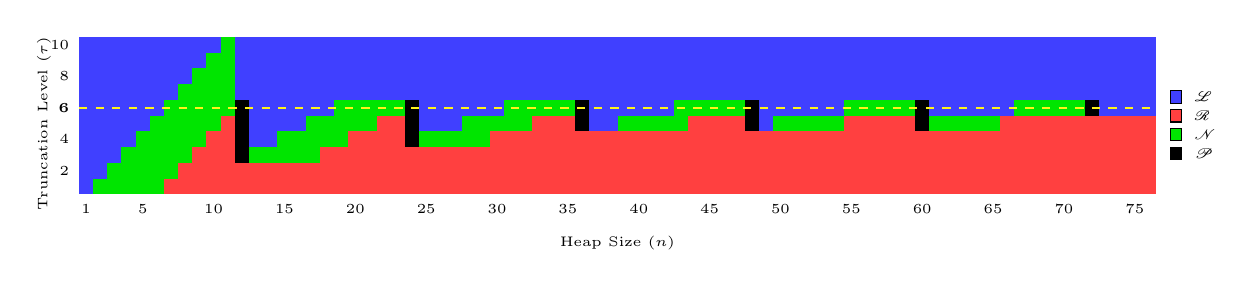
\begin{tikzpicture}[x=0.45cm, y=0.5cm, scale=0.4]
  % Colors
  \tikzset{fade/.style={fill opacity=1}}

  \colorlet{cL}{blue!75}
  \colorlet{cR}{red!75}
  \colorlet{cN}{green!90!black} % Off-white for visibility
  \colorlet{cP}{black}
  
  % Colored Blocks
  \fill[cL,fade] (0.5, 0.5) rectangle (1.5, 1.5);
  \fill[cN, fade] (1.5, 0.5) rectangle (2.5, 1.5);
  \fill[cN, fade] (2.5, 0.5) rectangle (3.5, 1.5);
  \fill[cN, fade] (3.5, 0.5) rectangle (4.5, 1.5);
  \fill[cN, fade] (4.5, 0.5) rectangle (5.5, 1.5);
  \fill[cN, fade] (5.5, 0.5) rectangle (6.5, 1.5);
  \fill[cR, fade] (6.5, 0.5) rectangle (7.5, 1.5);
  \fill[cR, fade] (7.5, 0.5) rectangle (8.5, 1.5);
  \fill[cR, fade] (8.5, 0.5) rectangle (9.5, 1.5);
  \fill[cR, fade] (9.5, 0.5) rectangle (10.5, 1.5);
  \fill[cR, fade] (10.5, 0.5) rectangle (11.5, 1.5);
  \fill[cR, fade] (11.5, 0.5) rectangle (12.5, 1.5);
  \fill[cR, fade] (12.5, 0.5) rectangle (13.5, 1.5);
  \fill[cR, fade] (13.5, 0.5) rectangle (14.5, 1.5);
  \fill[cR, fade] (14.5, 0.5) rectangle (15.5, 1.5);
  \fill[cR, fade] (15.5, 0.5) rectangle (16.5, 1.5);
  \fill[cR, fade] (16.5, 0.5) rectangle (17.5, 1.5);
  \fill[cR, fade] (17.5, 0.5) rectangle (18.5, 1.5);
  \fill[cR, fade] (18.5, 0.5) rectangle (19.5, 1.5);
  \fill[cR, fade] (19.5, 0.5) rectangle (20.5, 1.5);
  \fill[cR, fade] (20.5, 0.5) rectangle (21.5, 1.5);
  \fill[cR, fade] (21.5, 0.5) rectangle (22.5, 1.5);
  \fill[cR, fade] (22.5, 0.5) rectangle (23.5, 1.5);
  \fill[cR, fade] (23.5, 0.5) rectangle (24.5, 1.5);
  \fill[cR, fade] (24.5, 0.5) rectangle (25.5, 1.5);
  \fill[cR, fade] (25.5, 0.5) rectangle (26.5, 1.5);
  \fill[cR, fade] (26.5, 0.5) rectangle (27.5, 1.5);
  \fill[cR, fade] (27.5, 0.5) rectangle (28.5, 1.5);
  \fill[cR, fade] (28.5, 0.5) rectangle (29.5, 1.5);
  \fill[cR, fade] (29.5, 0.5) rectangle (30.5, 1.5);
  \fill[cR, fade] (30.5, 0.5) rectangle (31.5, 1.5);
  \fill[cR, fade] (31.5, 0.5) rectangle (32.5, 1.5);
  \fill[cR, fade] (32.5, 0.5) rectangle (33.5, 1.5);
  \fill[cR, fade] (33.5, 0.5) rectangle (34.5, 1.5);
  \fill[cR, fade] (34.5, 0.5) rectangle (35.5, 1.5);
  \fill[cR, fade] (35.5, 0.5) rectangle (36.5, 1.5);
  \fill[cR, fade] (36.5, 0.5) rectangle (37.5, 1.5);
  \fill[cR, fade] (37.5, 0.5) rectangle (38.5, 1.5);
  \fill[cR, fade] (38.5, 0.5) rectangle (39.5, 1.5);
  \fill[cR, fade] (39.5, 0.5) rectangle (40.5, 1.5);
  \fill[cR, fade] (40.5, 0.5) rectangle (41.5, 1.5);
  \fill[cR, fade] (41.5, 0.5) rectangle (42.5, 1.5);
  \fill[cR, fade] (42.5, 0.5) rectangle (43.5, 1.5);
  \fill[cR, fade] (43.5, 0.5) rectangle (44.5, 1.5);
  \fill[cR, fade] (44.5, 0.5) rectangle (45.5, 1.5);
  \fill[cR, fade] (45.5, 0.5) rectangle (46.5, 1.5);
  \fill[cR, fade] (46.5, 0.5) rectangle (47.5, 1.5);
  \fill[cR, fade] (47.5, 0.5) rectangle (48.5, 1.5);
  \fill[cR, fade] (48.5, 0.5) rectangle (49.5, 1.5);
  \fill[cR, fade] (49.5, 0.5) rectangle (50.5, 1.5);
  \fill[cR, fade] (50.5, 0.5) rectangle (51.5, 1.5);
  \fill[cR, fade] (51.5, 0.5) rectangle (52.5, 1.5);
  \fill[cR, fade] (52.5, 0.5) rectangle (53.5, 1.5);
  \fill[cR, fade] (53.5, 0.5) rectangle (54.5, 1.5);
  \fill[cR, fade] (54.5, 0.5) rectangle (55.5, 1.5);
  \fill[cR, fade] (55.5, 0.5) rectangle (56.5, 1.5);
  \fill[cR, fade] (56.5, 0.5) rectangle (57.5, 1.5);
  \fill[cR, fade] (57.5, 0.5) rectangle (58.5, 1.5);
  \fill[cR, fade] (58.5, 0.5) rectangle (59.5, 1.5);
  \fill[cR, fade] (59.5, 0.5) rectangle (60.5, 1.5);
  \fill[cR, fade] (60.5, 0.5) rectangle (61.5, 1.5);
  \fill[cR, fade] (61.5, 0.5) rectangle (62.5, 1.5);
  \fill[cR, fade] (62.5, 0.5) rectangle (63.5, 1.5);
  \fill[cR, fade] (63.5, 0.5) rectangle (64.5, 1.5);
  \fill[cR, fade] (64.5, 0.5) rectangle (65.5, 1.5);
  \fill[cR, fade] (65.5, 0.5) rectangle (66.5, 1.5);
  \fill[cR, fade] (66.5, 0.5) rectangle (67.5, 1.5);
  \fill[cR, fade] (67.5, 0.5) rectangle (68.5, 1.5);
  \fill[cR, fade] (68.5, 0.5) rectangle (69.5, 1.5);
  \fill[cR, fade] (69.5, 0.5) rectangle (70.5, 1.5);
  \fill[cR, fade] (70.5, 0.5) rectangle (71.5, 1.5);
  \fill[cR, fade] (71.5, 0.5) rectangle (72.5, 1.5);
  \fill[cR, fade] (72.5, 0.5) rectangle (73.5, 1.5);
  \fill[cR, fade] (73.5, 0.5) rectangle (74.5, 1.5);
  \fill[cR, fade] (74.5, 0.5) rectangle (75.5, 1.5);
  \fill[cR, fade] (75.5, 0.5) rectangle (76.5, 1.5);
  \fill[cL, fade] (0.5, 1.5) rectangle (1.5, 2.5);
  \fill[cL, fade] (1.5, 1.5) rectangle (2.5, 2.5);
  \fill[cN, fade] (2.5, 1.5) rectangle (3.5, 2.5);
  \fill[cN, fade] (3.5, 1.5) rectangle (4.5, 2.5);
  \fill[cN, fade] (4.5, 1.5) rectangle (5.5, 2.5);
  \fill[cN, fade] (5.5, 1.5) rectangle (6.5, 2.5);
  \fill[cN, fade] (6.5, 1.5) rectangle (7.5, 2.5);
  \fill[cR, fade] (7.5, 1.5) rectangle (8.5, 2.5);
  \fill[cR, fade] (8.5, 1.5) rectangle (9.5, 2.5);
  \fill[cR, fade] (9.5, 1.5) rectangle (10.5, 2.5);
  \fill[cR, fade] (10.5, 1.5) rectangle (11.5, 2.5);
  \fill[cR, fade] (11.5, 1.5) rectangle (12.5, 2.5);
  \fill[cR, fade] (12.5, 1.5) rectangle (13.5, 2.5);
  \fill[cR, fade] (13.5, 1.5) rectangle (14.5, 2.5);
  \fill[cR, fade] (14.5, 1.5) rectangle (15.5, 2.5);
  \fill[cR, fade] (15.5, 1.5) rectangle (16.5, 2.5);
  \fill[cR, fade] (16.5, 1.5) rectangle (17.5, 2.5);
  \fill[cR, fade] (17.5, 1.5) rectangle (18.5, 2.5);
  \fill[cR, fade] (18.5, 1.5) rectangle (19.5, 2.5);
  \fill[cR, fade] (19.5, 1.5) rectangle (20.5, 2.5);
  \fill[cR, fade] (20.5, 1.5) rectangle (21.5, 2.5);
  \fill[cR, fade] (21.5, 1.5) rectangle (22.5, 2.5);
  \fill[cR, fade] (22.5, 1.5) rectangle (23.5, 2.5);
  \fill[cR, fade] (23.5, 1.5) rectangle (24.5, 2.5);
  \fill[cR, fade] (24.5, 1.5) rectangle (25.5, 2.5);
  \fill[cR, fade] (25.5, 1.5) rectangle (26.5, 2.5);
  \fill[cR, fade] (26.5, 1.5) rectangle (27.5, 2.5);
  \fill[cR, fade] (27.5, 1.5) rectangle (28.5, 2.5);
  \fill[cR, fade] (28.5, 1.5) rectangle (29.5, 2.5);
  \fill[cR, fade] (29.5, 1.5) rectangle (30.5, 2.5);
  \fill[cR, fade] (30.5, 1.5) rectangle (31.5, 2.5);
  \fill[cR, fade] (31.5, 1.5) rectangle (32.5, 2.5);
  \fill[cR, fade] (32.5, 1.5) rectangle (33.5, 2.5);
  \fill[cR, fade] (33.5, 1.5) rectangle (34.5, 2.5);
  \fill[cR, fade] (34.5, 1.5) rectangle (35.5, 2.5);
  \fill[cR, fade] (35.5, 1.5) rectangle (36.5, 2.5);
  \fill[cR, fade] (36.5, 1.5) rectangle (37.5, 2.5);
  \fill[cR, fade] (37.5, 1.5) rectangle (38.5, 2.5);
  \fill[cR, fade] (38.5, 1.5) rectangle (39.5, 2.5);
  \fill[cR, fade] (39.5, 1.5) rectangle (40.5, 2.5);
  \fill[cR, fade] (40.5, 1.5) rectangle (41.5, 2.5);
  \fill[cR, fade] (41.5, 1.5) rectangle (42.5, 2.5);
  \fill[cR, fade] (42.5, 1.5) rectangle (43.5, 2.5);
  \fill[cR, fade] (43.5, 1.5) rectangle (44.5, 2.5);
  \fill[cR, fade] (44.5, 1.5) rectangle (45.5, 2.5);
  \fill[cR, fade] (45.5, 1.5) rectangle (46.5, 2.5);
  \fill[cR, fade] (46.5, 1.5) rectangle (47.5, 2.5);
  \fill[cR, fade] (47.5, 1.5) rectangle (48.5, 2.5);
  \fill[cR, fade] (48.5, 1.5) rectangle (49.5, 2.5);
  \fill[cR, fade] (49.5, 1.5) rectangle (50.5, 2.5);
  \fill[cR, fade] (50.5, 1.5) rectangle (51.5, 2.5);
  \fill[cR, fade] (51.5, 1.5) rectangle (52.5, 2.5);
  \fill[cR, fade] (52.5, 1.5) rectangle (53.5, 2.5);
  \fill[cR, fade] (53.5, 1.5) rectangle (54.5, 2.5);
  \fill[cR, fade] (54.5, 1.5) rectangle (55.5, 2.5);
  \fill[cR, fade] (55.5, 1.5) rectangle (56.5, 2.5);
  \fill[cR, fade] (56.5, 1.5) rectangle (57.5, 2.5);
  \fill[cR, fade] (57.5, 1.5) rectangle (58.5, 2.5);
  \fill[cR, fade] (58.5, 1.5) rectangle (59.5, 2.5);
  \fill[cR, fade] (59.5, 1.5) rectangle (60.5, 2.5);
  \fill[cR, fade] (60.5, 1.5) rectangle (61.5, 2.5);
  \fill[cR, fade] (61.5, 1.5) rectangle (62.5, 2.5);
  \fill[cR, fade] (62.5, 1.5) rectangle (63.5, 2.5);
  \fill[cR, fade] (63.5, 1.5) rectangle (64.5, 2.5);
  \fill[cR, fade] (64.5, 1.5) rectangle (65.5, 2.5);
  \fill[cR, fade] (65.5, 1.5) rectangle (66.5, 2.5);
  \fill[cR, fade] (66.5, 1.5) rectangle (67.5, 2.5);
  \fill[cR, fade] (67.5, 1.5) rectangle (68.5, 2.5);
  \fill[cR, fade] (68.5, 1.5) rectangle (69.5, 2.5);
  \fill[cR, fade] (69.5, 1.5) rectangle (70.5, 2.5);
  \fill[cR, fade] (70.5, 1.5) rectangle (71.5, 2.5);
  \fill[cR, fade] (71.5, 1.5) rectangle (72.5, 2.5);
  \fill[cR, fade] (72.5, 1.5) rectangle (73.5, 2.5);
  \fill[cR, fade] (73.5, 1.5) rectangle (74.5, 2.5);
  \fill[cR, fade] (74.5, 1.5) rectangle (75.5, 2.5);
  \fill[cR, fade] (75.5, 1.5) rectangle (76.5, 2.5);
  \fill[cL, fade] (0.5, 2.5) rectangle (1.5, 3.5);
  \fill[cL, fade] (1.5, 2.5) rectangle (2.5, 3.5);
  \fill[cL, fade] (2.5, 2.5) rectangle (3.5, 3.5);
  \fill[cN, fade] (3.5, 2.5) rectangle (4.5, 3.5);
  \fill[cN, fade] (4.5, 2.5) rectangle (5.5, 3.5);
  \fill[cN, fade] (5.5, 2.5) rectangle (6.5, 3.5);
  \fill[cN, fade] (6.5, 2.5) rectangle (7.5, 3.5);
  \fill[cN, fade] (7.5, 2.5) rectangle (8.5, 3.5);
  \fill[cR, fade] (8.5, 2.5) rectangle (9.5, 3.5);
  \fill[cR, fade] (9.5, 2.5) rectangle (10.5, 3.5);
  \fill[cR, fade] (10.5, 2.5) rectangle (11.5, 3.5);
  \fill[cP, fade] (11.5, 2.5) rectangle (12.5, 3.5);
  \fill[cN, fade] (12.5, 2.5) rectangle (13.5, 3.5);
  \fill[cN, fade] (13.5, 2.5) rectangle (14.5, 3.5);
  \fill[cN, fade] (14.5, 2.5) rectangle (15.5, 3.5);
  \fill[cN, fade] (15.5, 2.5) rectangle (16.5, 3.5);
  \fill[cN, fade] (16.5, 2.5) rectangle (17.5, 3.5);
  \fill[cR, fade] (17.5, 2.5) rectangle (18.5, 3.5);
  \fill[cR, fade] (18.5, 2.5) rectangle (19.5, 3.5);
  \fill[cR, fade] (19.5, 2.5) rectangle (20.5, 3.5);
  \fill[cR, fade] (20.5, 2.5) rectangle (21.5, 3.5);
  \fill[cR, fade] (21.5, 2.5) rectangle (22.5, 3.5);
  \fill[cR, fade] (22.5, 2.5) rectangle (23.5, 3.5);
  \fill[cR, fade] (23.5, 2.5) rectangle (24.5, 3.5);
  \fill[cR, fade] (24.5, 2.5) rectangle (25.5, 3.5);
  \fill[cR, fade] (25.5, 2.5) rectangle (26.5, 3.5);
  \fill[cR, fade] (26.5, 2.5) rectangle (27.5, 3.5);
  \fill[cR, fade] (27.5, 2.5) rectangle (28.5, 3.5);
  \fill[cR, fade] (28.5, 2.5) rectangle (29.5, 3.5);
  \fill[cR, fade] (29.5, 2.5) rectangle (30.5, 3.5);
  \fill[cR, fade] (30.5, 2.5) rectangle (31.5, 3.5);
  \fill[cR, fade] (31.5, 2.5) rectangle (32.5, 3.5);
  \fill[cR, fade] (32.5, 2.5) rectangle (33.5, 3.5);
  \fill[cR, fade] (33.5, 2.5) rectangle (34.5, 3.5);
  \fill[cR, fade] (34.5, 2.5) rectangle (35.5, 3.5);
  \fill[cR, fade] (35.5, 2.5) rectangle (36.5, 3.5);
  \fill[cR, fade] (36.5, 2.5) rectangle (37.5, 3.5);
  \fill[cR, fade] (37.5, 2.5) rectangle (38.5, 3.5);
  \fill[cR, fade] (38.5, 2.5) rectangle (39.5, 3.5);
  \fill[cR, fade] (39.5, 2.5) rectangle (40.5, 3.5);
  \fill[cR, fade] (40.5, 2.5) rectangle (41.5, 3.5);
  \fill[cR, fade] (41.5, 2.5) rectangle (42.5, 3.5);
  \fill[cR, fade] (42.5, 2.5) rectangle (43.5, 3.5);
  \fill[cR, fade] (43.5, 2.5) rectangle (44.5, 3.5);
  \fill[cR, fade] (44.5, 2.5) rectangle (45.5, 3.5);
  \fill[cR, fade] (45.5, 2.5) rectangle (46.5, 3.5);
  \fill[cR, fade] (46.5, 2.5) rectangle (47.5, 3.5);
  \fill[cR, fade] (47.5, 2.5) rectangle (48.5, 3.5);
  \fill[cR, fade] (48.5, 2.5) rectangle (49.5, 3.5);
  \fill[cR, fade] (49.5, 2.5) rectangle (50.5, 3.5);
  \fill[cR, fade] (50.5, 2.5) rectangle (51.5, 3.5);
  \fill[cR, fade] (51.5, 2.5) rectangle (52.5, 3.5);
  \fill[cR, fade] (52.5, 2.5) rectangle (53.5, 3.5);
  \fill[cR, fade] (53.5, 2.5) rectangle (54.5, 3.5);
  \fill[cR, fade] (54.5, 2.5) rectangle (55.5, 3.5);
  \fill[cR, fade] (55.5, 2.5) rectangle (56.5, 3.5);
  \fill[cR, fade] (56.5, 2.5) rectangle (57.5, 3.5);
  \fill[cR, fade] (57.5, 2.5) rectangle (58.5, 3.5);
  \fill[cR, fade] (58.5, 2.5) rectangle (59.5, 3.5);
  \fill[cR, fade] (59.5, 2.5) rectangle (60.5, 3.5);
  \fill[cR, fade] (60.5, 2.5) rectangle (61.5, 3.5);
  \fill[cR, fade] (61.5, 2.5) rectangle (62.5, 3.5);
  \fill[cR, fade] (62.5, 2.5) rectangle (63.5, 3.5);
  \fill[cR, fade] (63.5, 2.5) rectangle (64.5, 3.5);
  \fill[cR, fade] (64.5, 2.5) rectangle (65.5, 3.5);
  \fill[cR, fade] (65.5, 2.5) rectangle (66.5, 3.5);
  \fill[cR, fade] (66.5, 2.5) rectangle (67.5, 3.5);
  \fill[cR, fade] (67.5, 2.5) rectangle (68.5, 3.5);
  \fill[cR, fade] (68.5, 2.5) rectangle (69.5, 3.5);
  \fill[cR, fade] (69.5, 2.5) rectangle (70.5, 3.5);
  \fill[cR, fade] (70.5, 2.5) rectangle (71.5, 3.5);
  \fill[cR, fade] (71.5, 2.5) rectangle (72.5, 3.5);
  \fill[cR, fade] (72.5, 2.5) rectangle (73.5, 3.5);
  \fill[cR, fade] (73.5, 2.5) rectangle (74.5, 3.5);
  \fill[cR, fade] (74.5, 2.5) rectangle (75.5, 3.5);
  \fill[cR, fade] (75.5, 2.5) rectangle (76.5, 3.5);
  \fill[cL, fade] (0.5, 3.5) rectangle (1.5, 4.5);
  \fill[cL, fade] (1.5, 3.5) rectangle (2.5, 4.5);
  \fill[cL, fade] (2.5, 3.5) rectangle (3.5, 4.5);
  \fill[cL, fade] (3.5, 3.5) rectangle (4.5, 4.5);
  \fill[cN, fade] (4.5, 3.5) rectangle (5.5, 4.5);
  \fill[cN, fade] (5.5, 3.5) rectangle (6.5, 4.5);
  \fill[cN, fade] (6.5, 3.5) rectangle (7.5, 4.5);
  \fill[cN, fade] (7.5, 3.5) rectangle (8.5, 4.5);
  \fill[cN, fade] (8.5, 3.5) rectangle (9.5, 4.5);
  \fill[cR, fade] (9.5, 3.5) rectangle (10.5, 4.5);
  \fill[cR, fade] (10.5, 3.5) rectangle (11.5, 4.5);
  \fill[cP, fade] (11.5, 3.5) rectangle (12.5, 4.5);
  \fill[cL, fade] (12.5, 3.5) rectangle (13.5, 4.5);
  \fill[cL, fade] (13.5, 3.5) rectangle (14.5, 4.5);
  \fill[cN, fade] (14.5, 3.5) rectangle (15.5, 4.5);
  \fill[cN, fade] (15.5, 3.5) rectangle (16.5, 4.5);
  \fill[cN, fade] (16.5, 3.5) rectangle (17.5, 4.5);
  \fill[cN, fade] (17.5, 3.5) rectangle (18.5, 4.5);
  \fill[cN, fade] (18.5, 3.5) rectangle (19.5, 4.5);
  \fill[cR, fade] (19.5, 3.5) rectangle (20.5, 4.5);
  \fill[cR, fade] (20.5, 3.5) rectangle (21.5, 4.5);
  \fill[cR, fade] (21.5, 3.5) rectangle (22.5, 4.5);
  \fill[cR, fade] (22.5, 3.5) rectangle (23.5, 4.5);
  \fill[cP, fade] (23.5, 3.5) rectangle (24.5, 4.5);
  \fill[cN, fade] (24.5, 3.5) rectangle (25.5, 4.5);
  \fill[cN, fade] (25.5, 3.5) rectangle (26.5, 4.5);
  \fill[cN, fade] (26.5, 3.5) rectangle (27.5, 4.5);
  \fill[cN, fade] (27.5, 3.5) rectangle (28.5, 4.5);
  \fill[cN, fade] (28.5, 3.5) rectangle (29.5, 4.5);
  \fill[cR, fade] (29.5, 3.5) rectangle (30.5, 4.5);
  \fill[cR, fade] (30.5, 3.5) rectangle (31.5, 4.5);
  \fill[cR, fade] (31.5, 3.5) rectangle (32.5, 4.5);
  \fill[cR, fade] (32.5, 3.5) rectangle (33.5, 4.5);
  \fill[cR, fade] (33.5, 3.5) rectangle (34.5, 4.5);
  \fill[cR, fade] (34.5, 3.5) rectangle (35.5, 4.5);
  \fill[cR, fade] (35.5, 3.5) rectangle (36.5, 4.5);
  \fill[cR, fade] (36.5, 3.5) rectangle (37.5, 4.5);
  \fill[cR, fade] (37.5, 3.5) rectangle (38.5, 4.5);
  \fill[cR, fade] (38.5, 3.5) rectangle (39.5, 4.5);
  \fill[cR, fade] (39.5, 3.5) rectangle (40.5, 4.5);
  \fill[cR, fade] (40.5, 3.5) rectangle (41.5, 4.5);
  \fill[cR, fade] (41.5, 3.5) rectangle (42.5, 4.5);
  \fill[cR, fade] (42.5, 3.5) rectangle (43.5, 4.5);
  \fill[cR, fade] (43.5, 3.5) rectangle (44.5, 4.5);
  \fill[cR, fade] (44.5, 3.5) rectangle (45.5, 4.5);
  \fill[cR, fade] (45.5, 3.5) rectangle (46.5, 4.5);
  \fill[cR, fade] (46.5, 3.5) rectangle (47.5, 4.5);
  \fill[cR, fade] (47.5, 3.5) rectangle (48.5, 4.5);
  \fill[cR, fade] (48.5, 3.5) rectangle (49.5, 4.5);
  \fill[cR, fade] (49.5, 3.5) rectangle (50.5, 4.5);
  \fill[cR, fade] (50.5, 3.5) rectangle (51.5, 4.5);
  \fill[cR, fade] (51.5, 3.5) rectangle (52.5, 4.5);
  \fill[cR, fade] (52.5, 3.5) rectangle (53.5, 4.5);
  \fill[cR, fade] (53.5, 3.5) rectangle (54.5, 4.5);
  \fill[cR, fade] (54.5, 3.5) rectangle (55.5, 4.5);
  \fill[cR, fade] (55.5, 3.5) rectangle (56.5, 4.5);
  \fill[cR, fade] (56.5, 3.5) rectangle (57.5, 4.5);
  \fill[cR, fade] (57.5, 3.5) rectangle (58.5, 4.5);
  \fill[cR, fade] (58.5, 3.5) rectangle (59.5, 4.5);
  \fill[cR, fade] (59.5, 3.5) rectangle (60.5, 4.5);
  \fill[cR, fade] (60.5, 3.5) rectangle (61.5, 4.5);
  \fill[cR, fade] (61.5, 3.5) rectangle (62.5, 4.5);
  \fill[cR, fade] (62.5, 3.5) rectangle (63.5, 4.5);
  \fill[cR, fade] (63.5, 3.5) rectangle (64.5, 4.5);
  \fill[cR, fade] (64.5, 3.5) rectangle (65.5, 4.5);
  \fill[cR, fade] (65.5, 3.5) rectangle (66.5, 4.5);
  \fill[cR, fade] (66.5, 3.5) rectangle (67.5, 4.5);
  \fill[cR, fade] (67.5, 3.5) rectangle (68.5, 4.5);
  \fill[cR, fade] (68.5, 3.5) rectangle (69.5, 4.5);
  \fill[cR, fade] (69.5, 3.5) rectangle (70.5, 4.5);
  \fill[cR, fade] (70.5, 3.5) rectangle (71.5, 4.5);
  \fill[cR, fade] (71.5, 3.5) rectangle (72.5, 4.5);
  \fill[cR, fade] (72.5, 3.5) rectangle (73.5, 4.5);
  \fill[cR, fade] (73.5, 3.5) rectangle (74.5, 4.5);
  \fill[cR, fade] (74.5, 3.5) rectangle (75.5, 4.5);
  \fill[cR, fade] (75.5, 3.5) rectangle (76.5, 4.5);
  \fill[cL, fade] (0.5, 4.5) rectangle (1.5, 5.5);
  \fill[cL, fade] (1.5, 4.5) rectangle (2.5, 5.5);
  \fill[cL, fade] (2.5, 4.5) rectangle (3.5, 5.5);
  \fill[cL, fade] (3.5, 4.5) rectangle (4.5, 5.5);
  \fill[cL, fade] (4.5, 4.5) rectangle (5.5, 5.5);
  \fill[cN, fade] (5.5, 4.5) rectangle (6.5, 5.5);
  \fill[cN, fade] (6.5, 4.5) rectangle (7.5, 5.5);
  \fill[cN, fade] (7.5, 4.5) rectangle (8.5, 5.5);
  \fill[cN, fade] (8.5, 4.5) rectangle (9.5, 5.5);
  \fill[cN, fade] (9.5, 4.5) rectangle (10.5, 5.5);
  \fill[cR, fade] (10.5, 4.5) rectangle (11.5, 5.5);
  \fill[cP, fade] (11.5, 4.5) rectangle (12.5, 5.5);
  \fill[cL, fade] (12.5, 4.5) rectangle (13.5, 5.5);
  \fill[cL, fade] (13.5, 4.5) rectangle (14.5, 5.5);
  \fill[cL, fade] (14.5, 4.5) rectangle (15.5, 5.5);
  \fill[cL, fade] (15.5, 4.5) rectangle (16.5, 5.5);
  \fill[cN, fade] (16.5, 4.5) rectangle (17.5, 5.5);
  \fill[cN, fade] (17.5, 4.5) rectangle (18.5, 5.5);
  \fill[cN, fade] (18.5, 4.5) rectangle (19.5, 5.5);
  \fill[cN, fade] (19.5, 4.5) rectangle (20.5, 5.5);
  \fill[cN, fade] (20.5, 4.5) rectangle (21.5, 5.5);
  \fill[cR, fade] (21.5, 4.5) rectangle (22.5, 5.5);
  \fill[cR, fade] (22.5, 4.5) rectangle (23.5, 5.5);
  \fill[cP, fade] (23.5, 4.5) rectangle (24.5, 5.5);
  \fill[cL, fade] (24.5, 4.5) rectangle (25.5, 5.5);
  \fill[cL, fade] (25.5, 4.5) rectangle (26.5, 5.5);
  \fill[cL, fade] (26.5, 4.5) rectangle (27.5, 5.5);
  \fill[cN, fade] (27.5, 4.5) rectangle (28.5, 5.5);
  \fill[cN, fade] (28.5, 4.5) rectangle (29.5, 5.5);
  \fill[cN, fade] (29.5, 4.5) rectangle (30.5, 5.5);
  \fill[cN, fade] (30.5, 4.5) rectangle (31.5, 5.5);
  \fill[cN, fade] (31.5, 4.5) rectangle (32.5, 5.5);
  \fill[cR, fade] (32.5, 4.5) rectangle (33.5, 5.5);
  \fill[cR, fade] (33.5, 4.5) rectangle (34.5, 5.5);
  \fill[cR, fade] (34.5, 4.5) rectangle (35.5, 5.5);
  \fill[cP, fade] (35.5, 4.5) rectangle (36.5, 5.5);
  \fill[cL, fade] (36.5, 4.5) rectangle (37.5, 5.5);
  \fill[cL, fade] (37.5, 4.5) rectangle (38.5, 5.5);
  \fill[cN, fade] (38.5, 4.5) rectangle (39.5, 5.5);
  \fill[cN, fade] (39.5, 4.5) rectangle (40.5, 5.5);
  \fill[cN, fade] (40.5, 4.5) rectangle (41.5, 5.5);
  \fill[cN, fade] (41.5, 4.5) rectangle (42.5, 5.5);
  \fill[cN, fade] (42.5, 4.5) rectangle (43.5, 5.5);
  \fill[cR, fade] (43.5, 4.5) rectangle (44.5, 5.5);
  \fill[cR, fade] (44.5, 4.5) rectangle (45.5, 5.5);
  \fill[cR, fade] (45.5, 4.5) rectangle (46.5, 5.5);
  \fill[cR, fade] (46.5, 4.5) rectangle (47.5, 5.5);
  \fill[cP, fade] (47.5, 4.5) rectangle (48.5, 5.5);
  \fill[cL, fade] (48.5, 4.5) rectangle (49.5, 5.5);
  \fill[cN, fade] (49.5, 4.5) rectangle (50.5, 5.5);
  \fill[cN, fade] (50.5, 4.5) rectangle (51.5, 5.5);
  \fill[cN, fade] (51.5, 4.5) rectangle (52.5, 5.5);
  \fill[cN, fade] (52.5, 4.5) rectangle (53.5, 5.5);
  \fill[cN, fade] (53.5, 4.5) rectangle (54.5, 5.5);
  \fill[cR, fade] (54.5, 4.5) rectangle (55.5, 5.5);
  \fill[cR, fade] (55.5, 4.5) rectangle (56.5, 5.5);
  \fill[cR, fade] (56.5, 4.5) rectangle (57.5, 5.5);
  \fill[cR, fade] (57.5, 4.5) rectangle (58.5, 5.5);
  \fill[cR, fade] (58.5, 4.5) rectangle (59.5, 5.5);
  \fill[cP, fade] (59.5, 4.5) rectangle (60.5, 5.5);
  \fill[cN, fade] (60.5, 4.5) rectangle (61.5, 5.5);
  \fill[cN, fade] (61.5, 4.5) rectangle (62.5, 5.5);
  \fill[cN, fade] (62.5, 4.5) rectangle (63.5, 5.5);
  \fill[cN, fade] (63.5, 4.5) rectangle (64.5, 5.5);
  \fill[cN, fade] (64.5, 4.5) rectangle (65.5, 5.5);
  \fill[cR, fade] (65.5, 4.5) rectangle (66.5, 5.5);
  \fill[cR, fade] (66.5, 4.5) rectangle (67.5, 5.5);
  \fill[cR, fade] (67.5, 4.5) rectangle (68.5, 5.5);
  \fill[cR, fade] (68.5, 4.5) rectangle (69.5, 5.5);
  \fill[cR, fade] (69.5, 4.5) rectangle (70.5, 5.5);
  \fill[cR, fade] (70.5, 4.5) rectangle (71.5, 5.5);
  \fill[cR, fade] (71.5, 4.5) rectangle (72.5, 5.5);
  \fill[cR, fade] (72.5, 4.5) rectangle (73.5, 5.5);
  \fill[cR, fade] (73.5, 4.5) rectangle (74.5, 5.5);
  \fill[cR, fade] (74.5, 4.5) rectangle (75.5, 5.5);
  \fill[cR, fade] (75.5, 4.5) rectangle (76.5, 5.5);
  \fill[cL] (0.5, 5.5) rectangle (1.5, 6.5);
  \fill[cL] (1.5, 5.5) rectangle (2.5, 6.5);
  \fill[cL] (2.5, 5.5) rectangle (3.5, 6.5);
  \fill[cL] (3.5, 5.5) rectangle (4.5, 6.5);
  \fill[cL] (4.5, 5.5) rectangle (5.5, 6.5);
  \fill[cL] (5.5, 5.5) rectangle (6.5, 6.5);
  \fill[cN] (6.5, 5.5) rectangle (7.5, 6.5);
  \fill[cN] (7.5, 5.5) rectangle (8.5, 6.5);
  \fill[cN] (8.5, 5.5) rectangle (9.5, 6.5);
  \fill[cN] (9.5, 5.5) rectangle (10.5, 6.5);
  \fill[cN] (10.5, 5.5) rectangle (11.5, 6.5);
  \fill[cP] (11.5, 5.5) rectangle (12.5, 6.5);
  \fill[cL] (12.5, 5.5) rectangle (13.5, 6.5);
  \fill[cL] (13.5, 5.5) rectangle (14.5, 6.5);
  \fill[cL] (14.5, 5.5) rectangle (15.5, 6.5);
  \fill[cL] (15.5, 5.5) rectangle (16.5, 6.5);
  \fill[cL] (16.5, 5.5) rectangle (17.5, 6.5);
  \fill[cL] (17.5, 5.5) rectangle (18.5, 6.5);
  \fill[cN] (18.5, 5.5) rectangle (19.5, 6.5);
  \fill[cN] (19.5, 5.5) rectangle (20.5, 6.5);
  \fill[cN] (20.5, 5.5) rectangle (21.5, 6.5);
  \fill[cN] (21.5, 5.5) rectangle (22.5, 6.5);
  \fill[cN] (22.5, 5.5) rectangle (23.5, 6.5);
  \fill[cP] (23.5, 5.5) rectangle (24.5, 6.5);
  \fill[cL] (24.5, 5.5) rectangle (25.5, 6.5);
  \fill[cL] (25.5, 5.5) rectangle (26.5, 6.5);
  \fill[cL] (26.5, 5.5) rectangle (27.5, 6.5);
  \fill[cL] (27.5, 5.5) rectangle (28.5, 6.5);
  \fill[cL] (28.5, 5.5) rectangle (29.5, 6.5);
  \fill[cL] (29.5, 5.5) rectangle (30.5, 6.5);
  \fill[cN] (30.5, 5.5) rectangle (31.5, 6.5);
  \fill[cN] (31.5, 5.5) rectangle (32.5, 6.5);
  \fill[cN] (32.5, 5.5) rectangle (33.5, 6.5);
  \fill[cN] (33.5, 5.5) rectangle (34.5, 6.5);
  \fill[cN] (34.5, 5.5) rectangle (35.5, 6.5);
  \fill[cP] (35.5, 5.5) rectangle (36.5, 6.5);
  \fill[cL] (36.5, 5.5) rectangle (37.5, 6.5);
  \fill[cL] (37.5, 5.5) rectangle (38.5, 6.5);
  \fill[cL] (38.5, 5.5) rectangle (39.5, 6.5);
  \fill[cL] (39.5, 5.5) rectangle (40.5, 6.5);
  \fill[cL] (40.5, 5.5) rectangle (41.5, 6.5);
  \fill[cL] (41.5, 5.5) rectangle (42.5, 6.5);
  \fill[cN] (42.5, 5.5) rectangle (43.5, 6.5);
  \fill[cN] (43.5, 5.5) rectangle (44.5, 6.5);
  \fill[cN] (44.5, 5.5) rectangle (45.5, 6.5);
  \fill[cN] (45.5, 5.5) rectangle (46.5, 6.5);
  \fill[cN] (46.5, 5.5) rectangle (47.5, 6.5);
  \fill[cP] (47.5, 5.5) rectangle (48.5, 6.5);
  \fill[cL] (48.5, 5.5) rectangle (49.5, 6.5);
  \fill[cL] (49.5, 5.5) rectangle (50.5, 6.5);
  \fill[cL] (50.5, 5.5) rectangle (51.5, 6.5);
  \fill[cL] (51.5, 5.5) rectangle (52.5, 6.5);
  \fill[cL] (52.5, 5.5) rectangle (53.5, 6.5);
  \fill[cL] (53.5, 5.5) rectangle (54.5, 6.5);
  \fill[cN] (54.5, 5.5) rectangle (55.5, 6.5);
  \fill[cN] (55.5, 5.5) rectangle (56.5, 6.5);
  \fill[cN] (56.5, 5.5) rectangle (57.5, 6.5);
  \fill[cN] (57.5, 5.5) rectangle (58.5, 6.5);
  \fill[cN] (58.5, 5.5) rectangle (59.5, 6.5);
  \fill[cP] (59.5, 5.5) rectangle (60.5, 6.5);
  \fill[cL] (60.5, 5.5) rectangle (61.5, 6.5);
  \fill[cL] (61.5, 5.5) rectangle (62.5, 6.5);
  \fill[cL] (62.5, 5.5) rectangle (63.5, 6.5);
  \fill[cL] (63.5, 5.5) rectangle (64.5, 6.5);
  \fill[cL] (64.5, 5.5) rectangle (65.5, 6.5);
  \fill[cL] (65.5, 5.5) rectangle (66.5, 6.5);
  \fill[cN] (66.5, 5.5) rectangle (67.5, 6.5);
  \fill[cN] (67.5, 5.5) rectangle (68.5, 6.5);
  \fill[cN] (68.5, 5.5) rectangle (69.5, 6.5);
  \fill[cN] (69.5, 5.5) rectangle (70.5, 6.5);
  \fill[cN] (70.5, 5.5) rectangle (71.5, 6.5);
  \fill[cP] (71.5, 5.5) rectangle (72.5, 6.5);
  \fill[cL] (72.5, 5.5) rectangle (73.5, 6.5);
  \fill[cL] (73.5, 5.5) rectangle (74.5, 6.5);
  \fill[cL] (74.5, 5.5) rectangle (75.5, 6.5);
  \fill[cL] (75.5, 5.5) rectangle (76.5, 6.5);
  \fill[cL, fade] (0.5, 6.5) rectangle (1.5, 7.5);
  \fill[cL, fade] (1.5, 6.5) rectangle (2.5, 7.5);
  \fill[cL, fade] (2.5, 6.5) rectangle (3.5, 7.5);
  \fill[cL, fade] (3.5, 6.5) rectangle (4.5, 7.5);
  \fill[cL, fade] (4.5, 6.5) rectangle (5.5, 7.5);
  \fill[cL, fade] (5.5, 6.5) rectangle (6.5, 7.5);
  \fill[cL, fade] (6.5, 6.5) rectangle (7.5, 7.5);
  \fill[cN, fade] (7.5, 6.5) rectangle (8.5, 7.5);
  \fill[cN, fade] (8.5, 6.5) rectangle (9.5, 7.5);
  \fill[cN, fade] (9.5, 6.5) rectangle (10.5, 7.5);
  \fill[cN, fade] (10.5, 6.5) rectangle (11.5, 7.5);
  \fill[cL, fade] (11.5, 6.5) rectangle (12.5, 7.5);
  \fill[cL, fade] (12.5, 6.5) rectangle (13.5, 7.5);
  \fill[cL, fade] (13.5, 6.5) rectangle (14.5, 7.5);
  \fill[cL, fade] (14.5, 6.5) rectangle (15.5, 7.5);
  \fill[cL, fade] (15.5, 6.5) rectangle (16.5, 7.5);
  \fill[cL, fade] (16.5, 6.5) rectangle (17.5, 7.5);
  \fill[cL, fade] (17.5, 6.5) rectangle (18.5, 7.5);
  \fill[cL, fade] (18.5, 6.5) rectangle (19.5, 7.5);
  \fill[cL, fade] (19.5, 6.5) rectangle (20.5, 7.5);
  \fill[cL, fade] (20.5, 6.5) rectangle (21.5, 7.5);
  \fill[cL, fade] (21.5, 6.5) rectangle (22.5, 7.5);
  \fill[cL, fade] (22.5, 6.5) rectangle (23.5, 7.5);
  \fill[cL, fade] (23.5, 6.5) rectangle (24.5, 7.5);
  \fill[cL, fade] (24.5, 6.5) rectangle (25.5, 7.5);
  \fill[cL, fade] (25.5, 6.5) rectangle (26.5, 7.5);
  \fill[cL, fade] (26.5, 6.5) rectangle (27.5, 7.5);
  \fill[cL, fade] (27.5, 6.5) rectangle (28.5, 7.5);
  \fill[cL, fade] (28.5, 6.5) rectangle (29.5, 7.5);
  \fill[cL, fade] (29.5, 6.5) rectangle (30.5, 7.5);
  \fill[cL, fade] (30.5, 6.5) rectangle (31.5, 7.5);
  \fill[cL, fade] (31.5, 6.5) rectangle (32.5, 7.5);
  \fill[cL, fade] (32.5, 6.5) rectangle (33.5, 7.5);
  \fill[cL, fade] (33.5, 6.5) rectangle (34.5, 7.5);
  \fill[cL, fade] (34.5, 6.5) rectangle (35.5, 7.5);
  \fill[cL, fade] (35.5, 6.5) rectangle (36.5, 7.5);
  \fill[cL, fade] (36.5, 6.5) rectangle (37.5, 7.5);
  \fill[cL, fade] (37.5, 6.5) rectangle (38.5, 7.5);
  \fill[cL, fade] (38.5, 6.5) rectangle (39.5, 7.5);
  \fill[cL, fade] (39.5, 6.5) rectangle (40.5, 7.5);
  \fill[cL, fade] (40.5, 6.5) rectangle (41.5, 7.5);
  \fill[cL, fade] (41.5, 6.5) rectangle (42.5, 7.5);
  \fill[cL, fade] (42.5, 6.5) rectangle (43.5, 7.5);
  \fill[cL, fade] (43.5, 6.5) rectangle (44.5, 7.5);
  \fill[cL, fade] (44.5, 6.5) rectangle (45.5, 7.5);
  \fill[cL, fade] (45.5, 6.5) rectangle (46.5, 7.5);
  \fill[cL, fade] (46.5, 6.5) rectangle (47.5, 7.5);
  \fill[cL, fade] (47.5, 6.5) rectangle (48.5, 7.5);
  \fill[cL, fade] (48.5, 6.5) rectangle (49.5, 7.5);
  \fill[cL, fade] (49.5, 6.5) rectangle (50.5, 7.5);
  \fill[cL, fade] (50.5, 6.5) rectangle (51.5, 7.5);
  \fill[cL, fade] (51.5, 6.5) rectangle (52.5, 7.5);
  \fill[cL, fade] (52.5, 6.5) rectangle (53.5, 7.5);
  \fill[cL, fade] (53.5, 6.5) rectangle (54.5, 7.5);
  \fill[cL, fade] (54.5, 6.5) rectangle (55.5, 7.5);
  \fill[cL, fade] (55.5, 6.5) rectangle (56.5, 7.5);
  \fill[cL, fade] (56.5, 6.5) rectangle (57.5, 7.5);
  \fill[cL, fade] (57.5, 6.5) rectangle (58.5, 7.5);
  \fill[cL, fade] (58.5, 6.5) rectangle (59.5, 7.5);
  \fill[cL, fade] (59.5, 6.5) rectangle (60.5, 7.5);
  \fill[cL, fade] (60.5, 6.5) rectangle (61.5, 7.5);
  \fill[cL, fade] (61.5, 6.5) rectangle (62.5, 7.5);
  \fill[cL, fade] (62.5, 6.5) rectangle (63.5, 7.5);
  \fill[cL, fade] (63.5, 6.5) rectangle (64.5, 7.5);
  \fill[cL, fade] (64.5, 6.5) rectangle (65.5, 7.5);
  \fill[cL, fade] (65.5, 6.5) rectangle (66.5, 7.5);
  \fill[cL, fade] (66.5, 6.5) rectangle (67.5, 7.5);
  \fill[cL, fade] (67.5, 6.5) rectangle (68.5, 7.5);
  \fill[cL, fade] (68.5, 6.5) rectangle (69.5, 7.5);
  \fill[cL, fade] (69.5, 6.5) rectangle (70.5, 7.5);
  \fill[cL, fade] (70.5, 6.5) rectangle (71.5, 7.5);
  \fill[cL, fade] (71.5, 6.5) rectangle (72.5, 7.5);
  \fill[cL, fade] (72.5, 6.5) rectangle (73.5, 7.5);
  \fill[cL, fade] (73.5, 6.5) rectangle (74.5, 7.5);
  \fill[cL, fade] (74.5, 6.5) rectangle (75.5, 7.5);
  \fill[cL, fade] (75.5, 6.5) rectangle (76.5, 7.5);
  \fill[cL, fade] (0.5, 7.5) rectangle (1.5, 8.5);
  \fill[cL, fade] (1.5, 7.5) rectangle (2.5, 8.5);
  \fill[cL, fade] (2.5, 7.5) rectangle (3.5, 8.5);
  \fill[cL, fade] (3.5, 7.5) rectangle (4.5, 8.5);
  \fill[cL, fade] (4.5, 7.5) rectangle (5.5, 8.5);
  \fill[cL, fade] (5.5, 7.5) rectangle (6.5, 8.5);
  \fill[cL, fade] (6.5, 7.5) rectangle (7.5, 8.5);
  \fill[cL, fade] (7.5, 7.5) rectangle (8.5, 8.5);
  \fill[cN, fade] (8.5, 7.5) rectangle (9.5, 8.5);
  \fill[cN, fade] (9.5, 7.5) rectangle (10.5, 8.5);
  \fill[cN, fade] (10.5, 7.5) rectangle (11.5, 8.5);
  \fill[cL, fade] (11.5, 7.5) rectangle (12.5, 8.5);
  \fill[cL, fade] (12.5, 7.5) rectangle (13.5, 8.5);
  \fill[cL, fade] (13.5, 7.5) rectangle (14.5, 8.5);
  \fill[cL, fade] (14.5, 7.5) rectangle (15.5, 8.5);
  \fill[cL, fade] (15.5, 7.5) rectangle (16.5, 8.5);
  \fill[cL, fade] (16.5, 7.5) rectangle (17.5, 8.5);
  \fill[cL, fade] (17.5, 7.5) rectangle (18.5, 8.5);
  \fill[cL, fade] (18.5, 7.5) rectangle (19.5, 8.5);
  \fill[cL, fade] (19.5, 7.5) rectangle (20.5, 8.5);
  \fill[cL, fade] (20.5, 7.5) rectangle (21.5, 8.5);
  \fill[cL, fade] (21.5, 7.5) rectangle (22.5, 8.5);
  \fill[cL, fade] (22.5, 7.5) rectangle (23.5, 8.5);
  \fill[cL, fade] (23.5, 7.5) rectangle (24.5, 8.5);
  \fill[cL, fade] (24.5, 7.5) rectangle (25.5, 8.5);
  \fill[cL, fade] (25.5, 7.5) rectangle (26.5, 8.5);
  \fill[cL, fade] (26.5, 7.5) rectangle (27.5, 8.5);
  \fill[cL, fade] (27.5, 7.5) rectangle (28.5, 8.5);
  \fill[cL, fade] (28.5, 7.5) rectangle (29.5, 8.5);
  \fill[cL, fade] (29.5, 7.5) rectangle (30.5, 8.5);
  \fill[cL, fade] (30.5, 7.5) rectangle (31.5, 8.5);
  \fill[cL, fade] (31.5, 7.5) rectangle (32.5, 8.5);
  \fill[cL, fade] (32.5, 7.5) rectangle (33.5, 8.5);
  \fill[cL, fade] (33.5, 7.5) rectangle (34.5, 8.5);
  \fill[cL, fade] (34.5, 7.5) rectangle (35.5, 8.5);
  \fill[cL, fade] (35.5, 7.5) rectangle (36.5, 8.5);
  \fill[cL, fade] (36.5, 7.5) rectangle (37.5, 8.5);
  \fill[cL, fade] (37.5, 7.5) rectangle (38.5, 8.5);
  \fill[cL, fade] (38.5, 7.5) rectangle (39.5, 8.5);
  \fill[cL, fade] (39.5, 7.5) rectangle (40.5, 8.5);
  \fill[cL, fade] (40.5, 7.5) rectangle (41.5, 8.5);
  \fill[cL, fade] (41.5, 7.5) rectangle (42.5, 8.5);
  \fill[cL, fade] (42.5, 7.5) rectangle (43.5, 8.5);
  \fill[cL, fade] (43.5, 7.5) rectangle (44.5, 8.5);
  \fill[cL, fade] (44.5, 7.5) rectangle (45.5, 8.5);
  \fill[cL, fade] (45.5, 7.5) rectangle (46.5, 8.5);
  \fill[cL, fade] (46.5, 7.5) rectangle (47.5, 8.5);
  \fill[cL, fade] (47.5, 7.5) rectangle (48.5, 8.5);
  \fill[cL, fade] (48.5, 7.5) rectangle (49.5, 8.5);
  \fill[cL, fade] (49.5, 7.5) rectangle (50.5, 8.5);
  \fill[cL, fade] (50.5, 7.5) rectangle (51.5, 8.5);
  \fill[cL, fade] (51.5, 7.5) rectangle (52.5, 8.5);
  \fill[cL, fade] (52.5, 7.5) rectangle (53.5, 8.5);
  \fill[cL, fade] (53.5, 7.5) rectangle (54.5, 8.5);
  \fill[cL, fade] (54.5, 7.5) rectangle (55.5, 8.5);
  \fill[cL, fade] (55.5, 7.5) rectangle (56.5, 8.5);
  \fill[cL, fade] (56.5, 7.5) rectangle (57.5, 8.5);
  \fill[cL, fade] (57.5, 7.5) rectangle (58.5, 8.5);
  \fill[cL, fade] (58.5, 7.5) rectangle (59.5, 8.5);
  \fill[cL, fade] (59.5, 7.5) rectangle (60.5, 8.5);
  \fill[cL, fade] (60.5, 7.5) rectangle (61.5, 8.5);
  \fill[cL, fade] (61.5, 7.5) rectangle (62.5, 8.5);
  \fill[cL, fade] (62.5, 7.5) rectangle (63.5, 8.5);
  \fill[cL, fade] (63.5, 7.5) rectangle (64.5, 8.5);
  \fill[cL, fade] (64.5, 7.5) rectangle (65.5, 8.5);
  \fill[cL, fade] (65.5, 7.5) rectangle (66.5, 8.5);
  \fill[cL, fade] (66.5, 7.5) rectangle (67.5, 8.5);
  \fill[cL, fade] (67.5, 7.5) rectangle (68.5, 8.5);
  \fill[cL, fade] (68.5, 7.5) rectangle (69.5, 8.5);
  \fill[cL, fade] (69.5, 7.5) rectangle (70.5, 8.5);
  \fill[cL, fade] (70.5, 7.5) rectangle (71.5, 8.5);
  \fill[cL, fade] (71.5, 7.5) rectangle (72.5, 8.5);
  \fill[cL, fade] (72.5, 7.5) rectangle (73.5, 8.5);
  \fill[cL, fade] (73.5, 7.5) rectangle (74.5, 8.5);
  \fill[cL, fade] (74.5, 7.5) rectangle (75.5, 8.5);
  \fill[cL, fade] (75.5, 7.5) rectangle (76.5, 8.5);
  \fill[cL, fade] (0.5, 8.5) rectangle (1.5, 9.5);
  \fill[cL, fade] (1.5, 8.5) rectangle (2.5, 9.5);
  \fill[cL, fade] (2.5, 8.5) rectangle (3.5, 9.5);
  \fill[cL, fade] (3.5, 8.5) rectangle (4.5, 9.5);
  \fill[cL, fade] (4.5, 8.5) rectangle (5.5, 9.5);
  \fill[cL, fade] (5.5, 8.5) rectangle (6.5, 9.5);
  \fill[cL, fade] (6.5, 8.5) rectangle (7.5, 9.5);
  \fill[cL, fade] (7.5, 8.5) rectangle (8.5, 9.5);
  \fill[cL, fade] (8.5, 8.5) rectangle (9.5, 9.5);
  \fill[cN, fade] (9.5, 8.5) rectangle (10.5, 9.5);
  \fill[cN, fade] (10.5, 8.5) rectangle (11.5, 9.5);
  \fill[cL, fade] (11.5, 8.5) rectangle (12.5, 9.5);
  \fill[cL, fade] (12.5, 8.5) rectangle (13.5, 9.5);
  \fill[cL, fade] (13.5, 8.5) rectangle (14.5, 9.5);
  \fill[cL, fade] (14.5, 8.5) rectangle (15.5, 9.5);
  \fill[cL, fade] (15.5, 8.5) rectangle (16.5, 9.5);
  \fill[cL, fade] (16.5, 8.5) rectangle (17.5, 9.5);
  \fill[cL, fade] (17.5, 8.5) rectangle (18.5, 9.5);
  \fill[cL, fade] (18.5, 8.5) rectangle (19.5, 9.5);
  \fill[cL, fade] (19.5, 8.5) rectangle (20.5, 9.5);
  \fill[cL, fade] (20.5, 8.5) rectangle (21.5, 9.5);
  \fill[cL, fade] (21.5, 8.5) rectangle (22.5, 9.5);
  \fill[cL, fade] (22.5, 8.5) rectangle (23.5, 9.5);
  \fill[cL, fade] (23.5, 8.5) rectangle (24.5, 9.5);
  \fill[cL, fade] (24.5, 8.5) rectangle (25.5, 9.5);
  \fill[cL, fade] (25.5, 8.5) rectangle (26.5, 9.5);
  \fill[cL, fade] (26.5, 8.5) rectangle (27.5, 9.5);
  \fill[cL, fade] (27.5, 8.5) rectangle (28.5, 9.5);
  \fill[cL, fade] (28.5, 8.5) rectangle (29.5, 9.5);
  \fill[cL, fade] (29.5, 8.5) rectangle (30.5, 9.5);
  \fill[cL, fade] (30.5, 8.5) rectangle (31.5, 9.5);
  \fill[cL, fade] (31.5, 8.5) rectangle (32.5, 9.5);
  \fill[cL, fade] (32.5, 8.5) rectangle (33.5, 9.5);
  \fill[cL, fade] (33.5, 8.5) rectangle (34.5, 9.5);
  \fill[cL, fade] (34.5, 8.5) rectangle (35.5, 9.5);
  \fill[cL, fade] (35.5, 8.5) rectangle (36.5, 9.5);
  \fill[cL, fade] (36.5, 8.5) rectangle (37.5, 9.5);
  \fill[cL, fade] (37.5, 8.5) rectangle (38.5, 9.5);
  \fill[cL, fade] (38.5, 8.5) rectangle (39.5, 9.5);
  \fill[cL, fade] (39.5, 8.5) rectangle (40.5, 9.5);
  \fill[cL, fade] (40.5, 8.5) rectangle (41.5, 9.5);
  \fill[cL, fade] (41.5, 8.5) rectangle (42.5, 9.5);
  \fill[cL, fade] (42.5, 8.5) rectangle (43.5, 9.5);
  \fill[cL, fade] (43.5, 8.5) rectangle (44.5, 9.5);
  \fill[cL, fade] (44.5, 8.5) rectangle (45.5, 9.5);
  \fill[cL, fade] (45.5, 8.5) rectangle (46.5, 9.5);
  \fill[cL, fade] (46.5, 8.5) rectangle (47.5, 9.5);
  \fill[cL, fade] (47.5, 8.5) rectangle (48.5, 9.5);
  \fill[cL, fade] (48.5, 8.5) rectangle (49.5, 9.5);
  \fill[cL, fade] (49.5, 8.5) rectangle (50.5, 9.5);
  \fill[cL, fade] (50.5, 8.5) rectangle (51.5, 9.5);
  \fill[cL, fade] (51.5, 8.5) rectangle (52.5, 9.5);
  \fill[cL, fade] (52.5, 8.5) rectangle (53.5, 9.5);
  \fill[cL, fade] (53.5, 8.5) rectangle (54.5, 9.5);
  \fill[cL, fade] (54.5, 8.5) rectangle (55.5, 9.5);
  \fill[cL, fade] (55.5, 8.5) rectangle (56.5, 9.5);
  \fill[cL, fade] (56.5, 8.5) rectangle (57.5, 9.5);
  \fill[cL, fade] (57.5, 8.5) rectangle (58.5, 9.5);
  \fill[cL, fade] (58.5, 8.5) rectangle (59.5, 9.5);
  \fill[cL, fade] (59.5, 8.5) rectangle (60.5, 9.5);
  \fill[cL, fade] (60.5, 8.5) rectangle (61.5, 9.5);
  \fill[cL, fade] (61.5, 8.5) rectangle (62.5, 9.5);
  \fill[cL, fade] (62.5, 8.5) rectangle (63.5, 9.5);
  \fill[cL, fade] (63.5, 8.5) rectangle (64.5, 9.5);
  \fill[cL, fade] (64.5, 8.5) rectangle (65.5, 9.5);
  \fill[cL, fade] (65.5, 8.5) rectangle (66.5, 9.5);
  \fill[cL, fade] (66.5, 8.5) rectangle (67.5, 9.5);
  \fill[cL, fade] (67.5, 8.5) rectangle (68.5, 9.5);
  \fill[cL, fade] (68.5, 8.5) rectangle (69.5, 9.5);
  \fill[cL, fade] (69.5, 8.5) rectangle (70.5, 9.5);
  \fill[cL, fade] (70.5, 8.5) rectangle (71.5, 9.5);
  \fill[cL, fade] (71.5, 8.5) rectangle (72.5, 9.5);
  \fill[cL, fade] (72.5, 8.5) rectangle (73.5, 9.5);
  \fill[cL, fade] (73.5, 8.5) rectangle (74.5, 9.5);
  \fill[cL, fade] (74.5, 8.5) rectangle (75.5, 9.5);
  \fill[cL, fade] (75.5, 8.5) rectangle (76.5, 9.5);
  \fill[cL, fade] (0.5, 9.5) rectangle (1.5, 10.5);
  \fill[cL, fade] (1.5, 9.5) rectangle (2.5, 10.5);
  \fill[cL, fade] (2.5, 9.5) rectangle (3.5, 10.5);
  \fill[cL, fade] (3.5, 9.5) rectangle (4.5, 10.5);
  \fill[cL, fade] (4.5, 9.5) rectangle (5.5, 10.5);
  \fill[cL, fade] (5.5, 9.5) rectangle (6.5, 10.5);
  \fill[cL, fade] (6.5, 9.5) rectangle (7.5, 10.5);
  \fill[cL, fade] (7.5, 9.5) rectangle (8.5, 10.5);
  \fill[cL, fade] (8.5, 9.5) rectangle (9.5, 10.5);
  \fill[cL, fade] (9.5, 9.5) rectangle (10.5, 10.5);
  \fill[cN, fade] (10.5, 9.5) rectangle (11.5, 10.5);
  \fill[cL, fade] (11.5, 9.5) rectangle (12.5, 10.5);
  \fill[cL, fade] (12.5, 9.5) rectangle (13.5, 10.5);
  \fill[cL, fade] (13.5, 9.5) rectangle (14.5, 10.5);
  \fill[cL, fade] (14.5, 9.5) rectangle (15.5, 10.5);
  \fill[cL, fade] (15.5, 9.5) rectangle (16.5, 10.5);
  \fill[cL, fade] (16.5, 9.5) rectangle (17.5, 10.5);
  \fill[cL, fade] (17.5, 9.5) rectangle (18.5, 10.5);
  \fill[cL, fade] (18.5, 9.5) rectangle (19.5, 10.5);
  \fill[cL, fade] (19.5, 9.5) rectangle (20.5, 10.5);
  \fill[cL, fade] (20.5, 9.5) rectangle (21.5, 10.5);
  \fill[cL, fade] (21.5, 9.5) rectangle (22.5, 10.5);
  \fill[cL, fade] (22.5, 9.5) rectangle (23.5, 10.5);
  \fill[cL, fade] (23.5, 9.5) rectangle (24.5, 10.5);
  \fill[cL, fade] (24.5, 9.5) rectangle (25.5, 10.5);
  \fill[cL, fade] (25.5, 9.5) rectangle (26.5, 10.5);
  \fill[cL, fade] (26.5, 9.5) rectangle (27.5, 10.5);
  \fill[cL, fade] (27.5, 9.5) rectangle (28.5, 10.5);
  \fill[cL, fade] (28.5, 9.5) rectangle (29.5, 10.5);
  \fill[cL, fade] (29.5, 9.5) rectangle (30.5, 10.5);
  \fill[cL, fade] (30.5, 9.5) rectangle (31.5, 10.5);
  \fill[cL, fade] (31.5, 9.5) rectangle (32.5, 10.5);
  \fill[cL, fade] (32.5, 9.5) rectangle (33.5, 10.5);
  \fill[cL, fade] (33.5, 9.5) rectangle (34.5, 10.5);
  \fill[cL, fade] (34.5, 9.5) rectangle (35.5, 10.5);
  \fill[cL, fade] (35.5, 9.5) rectangle (36.5, 10.5);
  \fill[cL, fade] (36.5, 9.5) rectangle (37.5, 10.5);
  \fill[cL, fade] (37.5, 9.5) rectangle (38.5, 10.5);
  \fill[cL, fade] (38.5, 9.5) rectangle (39.5, 10.5);
  \fill[cL, fade] (39.5, 9.5) rectangle (40.5, 10.5);
  \fill[cL, fade] (40.5, 9.5) rectangle (41.5, 10.5);
  \fill[cL, fade] (41.5, 9.5) rectangle (42.5, 10.5);
  \fill[cL, fade] (42.5, 9.5) rectangle (43.5, 10.5);
  \fill[cL, fade] (43.5, 9.5) rectangle (44.5, 10.5);
  \fill[cL, fade] (44.5, 9.5) rectangle (45.5, 10.5);
  \fill[cL, fade] (45.5, 9.5) rectangle (46.5, 10.5);
  \fill[cL, fade] (46.5, 9.5) rectangle (47.5, 10.5);
  \fill[cL, fade] (47.5, 9.5) rectangle (48.5, 10.5);
  \fill[cL, fade] (48.5, 9.5) rectangle (49.5, 10.5);
  \fill[cL, fade] (49.5, 9.5) rectangle (50.5, 10.5);
  \fill[cL, fade] (50.5, 9.5) rectangle (51.5, 10.5);
  \fill[cL, fade] (51.5, 9.5) rectangle (52.5, 10.5);
  \fill[cL, fade] (52.5, 9.5) rectangle (53.5, 10.5);
  \fill[cL, fade] (53.5, 9.5) rectangle (54.5, 10.5);
  \fill[cL, fade] (54.5, 9.5) rectangle (55.5, 10.5);
  \fill[cL, fade] (55.5, 9.5) rectangle (56.5, 10.5);
  \fill[cL, fade] (56.5, 9.5) rectangle (57.5, 10.5);
  \fill[cL, fade] (57.5, 9.5) rectangle (58.5, 10.5);
  \fill[cL, fade] (58.5, 9.5) rectangle (59.5, 10.5);
  \fill[cL, fade] (59.5, 9.5) rectangle (60.5, 10.5);
  \fill[cL, fade] (60.5, 9.5) rectangle (61.5, 10.5);
  \fill[cL, fade] (61.5, 9.5) rectangle (62.5, 10.5);
  \fill[cL, fade] (62.5, 9.5) rectangle (63.5, 10.5);
  \fill[cL, fade] (63.5, 9.5) rectangle (64.5, 10.5);
  \fill[cL, fade] (64.5, 9.5) rectangle (65.5, 10.5);
  \fill[cL, fade] (65.5, 9.5) rectangle (66.5, 10.5);
  \fill[cL, fade] (66.5, 9.5) rectangle (67.5, 10.5);
  \fill[cL, fade] (67.5, 9.5) rectangle (68.5, 10.5);
  \fill[cL, fade] (68.5, 9.5) rectangle (69.5, 10.5);
  \fill[cL, fade] (69.5, 9.5) rectangle (70.5, 10.5);
  \fill[cL, fade] (70.5, 9.5) rectangle (71.5, 10.5);
  \fill[cL, fade] (71.5, 9.5) rectangle (72.5, 10.5);
  \fill[cL, fade] (72.5, 9.5) rectangle (73.5, 10.5);
  \fill[cL, fade] (73.5, 9.5) rectangle (74.5, 10.5);
  \fill[cL, fade] (74.5, 9.5) rectangle (75.5, 10.5);
  \fill[cL, fade] (75.5, 9.5) rectangle (76.5, 10.5);
  
  % Grid Lines
  % \draw[step=1.0, black, thin] (0.5, 0.5) grid (76.5, 10.5);
  
  % Highlight row \tau=4
  % \draw[line width=2pt, orange] (0.5, 3.5) rectangle (76.5, 4.5);
  
  % Axes Ticks
  \foreach \n in {1, 5, 10,..., 75} \node[below, font=\tiny] at (\n, 0.5) {\n};
  % \foreach \k in {1,2,...,9} \node[left, font=\scriptsize] at (0.5, \k) {\k};
  \foreach \k in {2,4,...,10}{
    \ifnum\k=6
        \node[left,font=\tiny] at (0.5,\k) {\textbf{\k}};
    \else
        \node[left,font=\tiny] at (0.5,\k) {\k};
    \fi
}
  % Axes Labels
  \node[below=0.4cm] at (38.5, 0.5) {\tiny Heap Size ($n$)};
  \node[rotate=90, above=1cm] at (-0.8, 0) {\tiny Truncation Level ($\tau$)};
    % \draw[yellow!90, line width=1pt]
    % (0.5,5.5) -- (76.5,5.5);

% \draw[yellow!90, line width=1pt]
    % (0.5,6.5) -- (76.5,6.5);

    \draw[yellow!90,dashed, line width=0.8pt]
    (0.5,6) -- (76.5,6);
  % Legend
  \begin{scope}[shift={(77.5, 5.5)}]
    % \node[right, font=\bfseries] at (0, 2.6) {\tiny Outcomes};
    \draw[fill=cL, fade] (0, 0.8) rectangle (0.8, 1.6); \node[right] at (1, 1.2) {\tiny $\mathscr{L}$};
    \draw[fill=cR, fade] (0, -0.4) rectangle (0.8, 0.4); \node[right] at (1, 0) {\tiny $\mathscr{R}$};
    \draw[fill=cN, fade] (0, -1.6) rectangle (0.8, -0.8); \node[right] at (1, -1.2) {\tiny $\mathscr{N}$};
    \draw[fill=cP, fade] (0, -2.8) rectangle (0.8, -2.0); \node[right] at (1, -2.4) {\tiny$\mathscr{P}$};
  \end{scope}
\end{tikzpicture}
\caption{Outcomes of $\ts_\tau(n; 5, 11)$. Blue, red, green, and black cells represent $\mathscr{L}$, $\mathscr{R}$, $\mathscr{N}$, and $\mathscr{P}$ outcomes, respectively. The yellow dashed line corresponds to truncation level $b-a$. \iffalse The row corresponding to the truncation level $b-a$ is highlighted.\fi }
\label{fig: outcome of ts_k(n;5,11)}
\end{figure}


\begin{example}
    % Consider $G=\ts_\tau(n;3,7)$. The outcome of $G$ for all $1\le \tau\le 6$ is given in Figure~\ref{fig: outcomes of ts(n,3,7)}. For $\tau=3$, the first block of the heap size is $[1,8]$, the second block is $[9,16]$, and so on. %the blocks are $[1,8],\; [9,16],\dots$. 
% In the first block, the outcome of {\sc TS} is $\lp$ for the first 3 heap sizes, $\np$ for the next 3, followed by 1 $\rp$ and 1 $\pp$. %$\beta^\text{th}$ block, where $\beta<\alpha=4$, 
In $H=\ts_4(n;5,11)$, the blocks are $[1,12],\;[13,24],\dots$ (refer to Figure~\ref{fig: outcome of ts_k(n;5,11)}). The first block starts with four $\lp$'s, followed by five $\np$'s, two $\rp$'s and one $\pp$.
\end{example} 

The first block contains $\tau$ consecutive $\lp$-positions. From one block to the next, the number of $\lp$-positions decreases by exactly $b-a-\tau$, while the number of $\rp$-positions increases by the same amount. %The numbers of $\np$- and $\pp$-positions remain unchanged.
% The first block has $\tau$ $\lp$-positions. As $\beta$ increases, the number of $\lp$-positions decreases by exactly $b-a-\tau$ from one block to the next. The number of $\rp$-positions increases by the same amount, while the numbers of $\np$- and $\pp$-positions remain fixed. 
This process continues until fewer than $b-a-\tau$  $\;\lp$-positions remain in a block. This occurs in the block with index
 \begin{align}
    \hbeta=\left \lfloor \frac{b-a}{b-a-\tau}\right\rfloor.\label{eq:betahat}
\end{align} 
% We denote this index by $\hbeta$.

%This happens at the block index   $\widehat \beta \coloneq\left \lfloor \frac{b-a}{b-a-\tau}\right\rfloor$, as in  \eqref{eq:beta}.  %We denote this particular index by $\hbeta$. 


 


% The parameter $\hbeta$ determines how long this block structure persists. 
% When $\tau$ is much smaller than $b-a$, the quantity $b-a-\tau$ is large, so the $\lp$-segment shrinks rapidly and the threshold $\hbeta$ is reached after only a few blocks. In contrast, when $\tau$ is close to $b-a$, the decrease is slow, and the same structured pattern persists over many blocks.

Unlike the preceding blocks, the $\hbeta$-th block contains no $\pp$-position. Instead, it begins with a segment of $\lp$-positions, followed by $a$ consecutive $\np$-positions, and all remaining positions in the block are $\rp$.
% In the $\widehat \beta$-th block, as in \eqref{eq:betahat}, the first few heap sizes have outcome $\lp$, the next $a$ heap sizes have outcome $\np$, and all remaining heap sizes have outcome $\rp$. The outcome corresponding to the last heap size in every block other than $\widehat \beta$ is $\pp$, but $\widehat \beta$-th block does not have any  $\pp$-position at all. 

%This also explains why the structured pattern persists for different numbers of blocks for different $\tau$. 
When $\tau$ is close to $b-a$, the quantity $b-a-\tau$ is small, so the $\lp$-segment shrinks slowly from one block to the next and consequently, $\hbeta$ is large. Conversely, when $\tau$ is much smaller than $b-a$, the decrease is much faster and hence, $\hbeta$ is small.
% In the next lemma, we describe the pattern of outcomes of $\ts_\tau(n; a, b)$ for smaller heap sizes when the truncation level is low ($\tau < b-a$). 

% For $\beta\le \hbeta$, we let $L_\beta$ denote the first heap size of $\beta^\text{th}$ block (that is, $L_\beta=(\beta-1)(b+1)+1)$), and we let $P_\beta$ denote the last heap size of $\beta^\text{th}$ block (that is, $\beta(b+1)$). We use $N_\beta$ and $R_\beta$ to denote the heap sizes from where $\np$-positions and $\rp$-positions start in that block, respectively. 

% For each block with index $\beta<\hbeta$, let $L_\beta$, $N_\beta$, $R_\beta$, and $P_\beta$ denote the heap sizes of the first $\lp$-, $\np$-, $\rp$-, and $\pp$-position in that block, respectively. For the $\hbeta$-th block, we similarly denote the heap sizes of the first $\lp$-, $\np$-, and $\rp$-position by $L_{\hbeta}$, $N_{\hbeta}$, and $R_{\hbeta}$, respectively. (There is no $P_{\hbeta}$ since $\hbeta$-th block contains no $\pp$-position.)

For each block with index $\beta<\hbeta$, we define \begin{align}
    L_\beta&\coloneq(\beta-1)(b+1)+1,\label{eq:L-beta}\\
    N_\beta&\coloneq\beta(a+\tau+1)-a,\label{eq:N-beta}\\
    R_\beta&\coloneq\beta(a+\tau+1),\label{eq:R-beta}\\
    P_\beta&\coloneq\beta(b+1).\label{eq:P-beta}
\end{align} In the next lemma, we will see that $L_\beta$, $N_\beta$, $R_\beta$, and $P_\beta$ are the heap sizes corresponding to the first $\lp$-, $\np$-, $\rp$-, and $\pp$-position in $\beta$-th block, respectively. 

% For the $\hbeta$-th block, we similarly denote the heap sizes of the first $\lp$-, $\np$-, and $\rp$-position by $L_{\hbeta}$, $N_{\hbeta}$, and $R_{\hbeta}$, respectively. (There is no $P_{\hbeta}$ since $\hbeta$-th block contains no $\pp$-position.)

% For $\beta\le \hbeta$, let $N_{1}^{\beta}$ and $N_{4}^{\beta}$ denote the first and the last heap size of the $\beta^\text{th}$ block, respectively (that is, $N_{1}^{\beta}=(\beta-1)(b+1)+1)$, and $N_{4}^{\beta}=\beta(b+1)$). We use $N_{2}^{\beta}$ and $N_{3}^{\beta}$ to denote the heap sizes from where $\np$-positions and $\rp$-positions start in that block, respectively.  We skip writing $\beta$ in the superscript, if it is clear from the context.
% For $\beta\le \hbeta$, let $L_\beta$ denote the first heap size of $\beta^\text{th}$ block (that is, $L_\beta=(\beta-1)(b+1)+1)$), and let $N_\beta$ denote the heap size from where $\np$-positions starts in that block. Similarly, let $R_\beta$ denote the heap size at which $\rp$-positions starts and $P_\beta$ denotes the last heap size of that block. 

% We divide the heap sizes into consecutive intervals of size $b+1$. The first interval contains heap sizes from $1$ to $b+1$, the second contains heap sizes from $b+2$ to $2(b+1)$, and so on, where $\beta \ge 1$ represents the interval number.

% Within each of these intervals—up to a certain limit $\hbeta$—the outcomes follow a clear, repeating pattern. First, there is a group of $\lp$ outcomes, followed by exactly $a$ outcomes of $\np$, then a group of $\rp$ outcomes, and finally a single $\pp$ outcome at the very end of the interval.

% As we move to larger intervals (as $\beta$ increases), the number of $\lp$ outcomes in each interval decreases by $b-a-\tau$ every time, while the number of $\rp$ outcomes increases by the same amount. The number of $\np$ outcomes (always $a$) and $\pp$ outcomes (always $1$) stays exactly the same. This behavior continues until there are no $\lp$ outcomes left in the interval.

% How long this pattern lasts depends on how close $\tau$ is to $b-a$. If $\tau$ is far below $b-a$, the number of $\lp$'s drops quickly, so we reach the limit $\hbeta$ very soon. If $\tau$ is close to $b-a$, the number of $\lp$'s decreases slowly, meaning this pattern lasts for a much longer range of heap sizes.
\begin{lemma}\label{lem: outcome ts below alpha block}
    Let $a,b$ and $\tau$ are positive integers such that $a<b$ and $\tau<b-a$. Then, for all $\beta<\hbeta$, %let 
    %     \begin{itemize}
    %     \item $L_\beta=(\beta-1)(b+1)+1$,
    %     \item $N_\beta=\beta(a+\tau+1)-a$, %=L_\beta-1+b-a-\beta(b-a-\tau)
    %     \item $R_\beta=\beta(a+\tau+1)$, %=N_\beta+a 
    %     \item $P_\beta=\beta(b+1)$. %=R_\beta+\beta(b-a-\tau)-1
    % \end{itemize}
    %Let %$\hbeta$ be such that $$\frac{(\hbeta-1)(b-a)-1}{\hbeta}<\tau\le \frac{\hbeta(b-a)-1}{\hbeta+1},$$ 
    %$\hbeta=\left \lfloor \frac{b-a}{b-a-\tau}\right\rfloor$
    %Then  %as in \eqref{eq:betahat},
    \begin{align*}
        o\big(\ts_\tau(n;a,b)\big)=\begin{cases}
            \lp & \text{ if } L_\beta \le  n<N_\beta ;\\
            \np & \text{ if } N_\beta\le  n< R_\beta;\\
            \rp & \text{ if } R_\beta\le  n< P_\beta;\\
            \pp & \text{ if } n=P_\beta.
        \end{cases}
    \end{align*}
\end{lemma}
\begin{proof}
    If $2\tau<b-a$, then $\hbeta=1$, and the statements holds vacuously. So, assume $2\tau\ge b-a$. We must prove that
    \begin{itemize}
        \item[(i)] Left wins $G$ if $L_\beta\le n< N_\beta$,
        \item[(ii)] First player wins $G$ if $N_\beta\le n< R_\beta$,
        \item[(iii)] Right wins $G$ if $R_\beta\le n< P_\beta$,
        \item[(iv)] Second player wins $G$ if $n=P_\beta$.
    \end{itemize}

    We first consider the case $\beta=1$. If $L_1\le n<P_1$, the statement holds using Lemma~\ref{lem: outcome TS heap<=b}. So let $n=P_1=b+1$: If Left starts, then any resulting position is either $\np$ or $\rp$ as $n-a>\tau+1=N_1$ and $n-1<P_1$. Thus, Right wins $G$. If Right starts, any resulting position is either $\lp$ or $\np$ as $n-b=1\ge L_1$ and $n-(\tau+1)\le a+\tau<R_1$. Thus, Left wins $G$. This completes the proof for $\beta=1$. 
    
    Now suppose $\beta>1$, i.e, $n\ge b+2$.

    % By induction, $L_{\beta-1}$, $N_{\beta-1},\;R_{\beta-1}$ and $P_{\beta-1}$ are as follows:
    % % Let $L_{\beta-1}$, $N_{\beta-1},\;R_{\beta-1}$ and $P_{\beta-1}$ are obtained from $L_\beta,N_\beta,R_\beta$ and $P_\beta$ respectively by replacing $\beta$ by $\beta-1$ in those. Thus
    % \begin{align*}
    %     L_{\beta-1}&=(\beta-2)(b+1)+1, \; & N_{\beta-1}&=(\beta-1)(a+\tau+1)-a,\\
    %     R_{\beta-1}&=(\beta-1)(a+\tau+1), \; & P_{\beta-1}&=(\beta-1)(b+1).
    % \end{align*}
    
    Consider item~(i).  Suppose first that Right starts in $G$ and moves to $G^R$. Denote the heap size of $G^R$ by $n_r$. Since $L_\beta\le n< N_\beta$, $$L_\beta-b\le n_r<N_\beta-(\tau+1).$$ By simple calculations, we get $L_\beta-b>L_{\beta-1}$ and $N_\beta-(\tau+1)=R_{\beta-1}$. Thus, $$L_{\beta-1}<n_r< R_{\beta-1}.$$ Hence, by induction, the outcome of $G^R$ is either $\lp$ or $\np$, and thus, Left wins playing first on $G^R$. Since $G^R$ is an arbitrary Right option, Left wins $G$. 
    
    Next suppose that Left starts in $G$. We claim that Left wins by removing 1 token. Let $G^L$ denote the Left option $\ts_\tau(n-1;a,b)$. If $n=L_\beta$, i.e., $n-1=P_{\beta-1}$, then outcome of $G^L$ is $\pp$ by induction and hence, Left wins $G$. Otherwise $L_\beta\le n-1< N_\beta-1$, and in this range, we already proved that Right loses as first player. Thus, Left wins $G$ by moving to $\ts_\tau(n-1;a,b)$.
    
    Consider item~(ii). First suppose that Left starts on $G$. Since the outcome of {\sc TS} is $\lp$ below the heap size $N_\beta$ by item~(i), Left wins if she can reach the heap size $N_\beta-1$. For this purpose, she needs to remove $n-N_\beta+1$ tokens %from the heap and wins as $o\left(\ts_\tau(N_\beta-1;a,b)\right)=\lp$ by item~(i). This is legal as 
    and this is possible as $$1\le n-N_\beta+1< R_\beta-N_\beta+1=a+1.$$ Therefore, Left wins $G$ by doing so. 
    
    Next suppose that Right starts on $G$. 
    %If $\beta=1$, then $\tau+1\le n\le \tau+a<b$, and Right wins by removing the full heap. Otherwise, 
    Right can win by reducing the heap size to $R_{\beta-1}$ by induction. For this purpose, Right needs to remove $n-R_{\beta-1}$ many tokens. Since $$\tau+1=N_\beta-R_{\beta-1}\le n-R_{\beta-1}<R_\beta-R_{\beta-1}=a+\tau+1\le b,$$ Right does so and wins $G$. % By induction, the outcome of $\ts_\tau(R_{\beta-1};a,b)$ is $\rp$, and hence Right wins.

    Consider item~(iii). Suppose Right starts on $G$. %If $\beta=1$, then $a+\tau+1\le n\le b$, and therefore, Right wins by removing the full heap. Otherwise, 
    By induction, Right wins if he can reach any heap size between $R_{\beta-1}$ and $P_{\beta-1}$, both included. We know \begin{align*}
        R_{\beta-1}&=R_\beta-(a+\tau+1),\\
        P_{\beta-1}&=P_\beta-(b+1).
    \end{align*}This implies $R_{\beta-1}+a+\tau+1\le n\le P_{\beta-1}+b$. Since all numbers from $a+\tau+1$ to $b$ are in the subtraction set of Right, he can always reach a heap size between $R_{\beta-1}$ and $P_{\beta-1}$, both included and thus, Right wins. 
    
    Now suppose Left starts on $G$ and her move leads to heap size $n_\ell$. Then $$N_\beta=R_\beta-a\le n_\ell< P_\beta-1.$$ We already proved that Right wins as first player on any of these heap sizes. Since, $n_\ell$ is arbitrary, Right wins $G$. 

    Consider item~(iv). Suppose Left starts on $G$ and move to heap size $n_\ell$. Then, $$N_\beta\le P_\beta-a\le n_\ell\le P_\beta-1.$$ We already proved that Right wins as first player on any of these heap sizes. Since $n_\ell$ is arbitrary, Right wins $G$. 
    
    Now suppose Right starts on $G$ and move to heap size $n_r$. Then, \begin{align}
        L_\beta\le P_\beta-b\le n_r&\le P_\beta-(\tau+1)\nonumber\\
        &=\beta(b+1)-(\tau+1)-R_\beta+R_\beta\nonumber\\
        &=\beta(b-a-\tau)-(\tau+1)+R_\beta\nonumber\\
        &<\frac{\tau+1}{b-a-\tau}(b-a-\tau)-(\tau+1)+R_\beta\label{eq:1}\\
        &=R_\beta\nonumber.
    \end{align}
    Equation~\eqref{eq:1} follows as $\beta\le \hbeta-1\le \frac{\tau}{b-a-\tau}<\frac{\tau+1}{b-a-\tau}$. We already proved that Left wins as first player on any of these heap sizes. Since, $n_r$ is arbitrary, Left wins $G$. 
\end{proof}

We now establish the outcome pattern of the $\widehat \beta$-th block. Similar to $L_\beta$, $N_\beta$, and $R_\beta$ defined in Equations~\eqref{eq:L-beta}, \eqref{eq:N-beta} and \eqref{eq:R-beta} for $\beta<\hbeta$, we define $L_{\hbeta}$, $N_{\hbeta}$, and $R_{\hbeta}$ for the $\hbeta$-th block as \begin{align}
    L_{\hbeta}&\coloneq(\hbeta-1)(b+1)+1,\\
    N_{\hbeta}&\coloneq\hbeta(a+\tau+1)-a,\\
    R_{\hbeta}&\coloneq\hbeta(a+\tau+1).
    % P_\beta&\coloneq\beta(b+1).
\end{align} In the next lemma, we will see that $L_{\hbeta}$, $N_{\hbeta}$, and $R_{\hbeta}$ are the heap sizes corresponding to the first $\lp$-, $\np$-, and $\rp$-position in the $\hbeta$-th block, respectively. We will also see that there is no $\pp$-position in this block.

% For the $\hbeta$-th block, we similarly denote the heap sizes of the first $\lp$-, $\np$-, and $\rp$-position by $L_{\hbeta}$, $N_{\hbeta}$, and $R_{\hbeta}$, respectively. (There is no $P_{\hbeta}$ since $\hbeta$-th block contains no $\pp$-position.) % Same as before, for fix  $a,b$ and $\tau$, the heap sizes are divided into blocks of size $b+1$. In the next lemma, we prove that in the $\hbeta^\text{th}$ block, the outcome of {\sc TS} for the first $\tau-(\hbeta-1)(b-a-\tau)$ heap sizes is $\lp$, the next $a$ heap sizes is $\np$ and the outcome of all the remaining heap sizes in that block is $\rp$. 

\begin{lemma}\label{lem: outcome ts in alpha block}
    Let $a,b$ and $\tau$ are positive integers such that $a<b$ and $\tau<b-a$. %Let %$\hbeta$ be such that $$\frac{(\hbeta-1)(b-a)-1}{\hbeta}<\tau\le \frac{\hbeta(b-a)-1}{\hbeta+1},$$ 
    %$\hbeta=\left \lfloor \frac{b-a}{b-a-\tau}\right\rfloor$, 
    %Let \begin{itemize}
        % \item $L_{\hbeta}=(\hbeta-1)(b+1)+1$,
        % \item $N_{\hbeta}=\hbeta(a+\tau+1)-a$, %=L_\beta-1+b-a-\alpha(b-a-\tau)
        % \item $R_{\hbeta}=\hbeta(a+\tau+1)$, %=N_\beta+a
        % % \item $P_{\hbeta}=\hbeta(b+1).$
    % \end{itemize} 
    Then \begin{align}
        o\big(\ts_\tau(n;a,b)\big)=\begin{cases}
            \lp & \text{ if } L_{\hbeta} \le  n<N_{\hbeta} ;\\
            \np & \text{ if } N_{\hbeta}\le  n< R_{\hbeta};\\
            \rp & \text{ if } R_{\hbeta}\le  n\le {\hbeta}(b+1).
        \end{cases}
    \end{align}
\end{lemma}
\begin{proof}
    It suffices to show the following:
    \begin{enumerate}
        \item Left wins $G$ if $L_{\hbeta}\le n<N_{\hbeta}$,
        \item First players wins $G$ if $N_{\hbeta}\le n<R_{\hbeta}$,
        \item Right wins $G$ if $R_{\hbeta}\le n< {\hbeta}(b+1)$,
        \item Right wins $G$ if $n={\hbeta}(b+1)$.
    \end{enumerate}
    We skip the proof of items~(1), (2) and (3), as they are similar to the proof of items~(i), (ii) and (iii) of Lemma~\ref{lem: outcome ts below alpha block}.  

    Let $n=\hbeta(b+1)$.  Suppose Right starts on $G$, then he wins by removing $n-R_{\hbeta}$ tokens from the heap as it leads to $\ts_\tau(R_{\hbeta};a,b)$, which is an $\rp$-position by item~(3); this is a legal move as $n-R_{\hbeta}<b$ and
\begin{align}
    n-R_{\hbeta}&={\hbeta}(b+1)-{\hbeta}(a+\tau+1)\nonumber\\
    &={\hbeta}(b-a-\tau)\nonumber\\
    &=\left\lfloor\frac{b-a}{b-a-\tau}\right\rfloor \cdot (b-a-\tau)\nonumber\\
    &>\left(\frac{b-a}{b-a-\tau}-1\right) \cdot (b-a-\tau) =\tau.\label{eq:2}
\end{align}
Now suppose that Left starts on $G$ and move to heap size $n_\ell$. Then $$n-a\le n_\ell<n,$$
where \begin{align*}n-a  &=  n-(R_{\hbeta}-N_{\hbeta}) \\
&={\hbeta}(b+1)-R_{\hbeta} +N_{\hbeta} \\
&> N_{\hbeta}.\end{align*} By items~(2) and (3), the outcome of $\ts_\tau(n_\ell;a,b)$ is either $\np$ or $\rp$, and hence, Right wins $G$.  This completes the proof.
\end{proof}

We have established the pattern of the outcomes of {\sc TS} up to the heap size $\hbeta(b+1)$; we now prove that all the remaining heap sizes are $\rp$-positions.

\begin{lemma}\label{lem: right dominating}
     Consider $G=\ts_\tau(n;a,b)$ where $a<b$ and $\tau<b-a$. Then  $G\in \rp$ for all $n\ge R_{\hbeta}$.
\end{lemma}
\begin{proof}
    We prove the statement by induction. %Let $L_{\hbeta},N_{\hbeta},$ and $R_{\hbeta}$ be the same as defined in Lemma~\ref{lem: outcome ts in alpha block}:
    % \begin{align*}
    %     L_{\hbeta}&=(\hbeta-1)(b+1)+1, \; & N_{\hbeta}&=\hbeta(a+\tau+1)-a,\; &
    %     R_{\hbeta}&=\hbeta(a+\tau+1).
    % \end{align*}
    The statement is true for $R_{\hbeta}\le n\le \hbeta(b+1)$ by Lemma~\ref{lem: outcome ts in alpha block}. So suppose $n>\hbeta(b+1)$. 
    
    Suppose first that Left starts on $G$ and move to heap size $n_\ell$. Then $$n_\ell>\hbeta(b+1)-a=\hbeta(b+1)-(R_{\hbeta}-N_{\hbeta})>N_{\hbeta}.$$ Therefore, by Lemma~\ref{lem: outcome ts in alpha block} and induction, the outcome of $\ts_\tau(n_\ell;a,b)$ is either $\np$ or $\rp$. Hence, Right wins this position as the next player. Since, $n_\ell$ is arbitrary, Right wins $G$. 
    
    Now suppose that Right starts on $G$ and removes $\hbeta(b+1)-R_{\hbeta}$ tokens. This is legal as $$\tau<\hbeta(b+1)-R_{\hbeta}<b,$$ by Equation~\eqref{eq:2}. %This results in heap size $n-(\hbeta(b+1)-R_{\hbeta})$. 
    Since $n>\hbeta(b+1)$, the resulting heap size is greater than $R_{\hbeta}$, and by induction, this position has outcome $\rp$. Hence, Right wins $G$. 
\end{proof}

We have find the outcomes of $\ts_\tau(n;a,b)$ for all small truncation levels ($\tau<b-a$) and proved that Right wins $\ts_\tau(n;a,b)$ for all sufficiently large $n$. However, this information is not enough to play strategically in a disjunctive sum of games. Additional information like atomic weight is required. In the next section, We compute the atomic weight of the {\sc TS} ruleset. 

\section{Atomic weights of Truncated Support}\label{sec: AW of TS} 
Table~\ref{tab:aw of ts(n,3,7)} suggests a pattern in the atomic weights of $\ts_\tau(n;3,7)$. For $\tau<b-a$, the pattern begins exactly at heap size 
$R_{\hbeta}=\hbeta(a+\tau+1)$, where $\hbeta=\left\lfloor\frac{b-a}{b-a-\tau}\right\rfloor$. By Theorem~\ref{thm: outcomes of TS}, starting from $R_{\hbeta}$, all larger heap sizes have outcome $\rp$. So, Right can delay playing as long as the heap size remains larger or equal to $R_{\hbeta}$.  Left can remove at most $a$ tokens per move, and thus the minimum number of moves required for Left to reduce the heap size below $R_{\hbeta}$ is: 
\[ 
\left\lceil\frac{n-(R_{\hbeta}-1)}{a}\right\rceil.
\] 
Thus, Right can delay his move exactly $\left\lceil\frac{n-(R_{\hbeta}\,-1)}{a}\right\rceil-1=\left\lfloor\frac{n-R_{\hbeta}}{a}\right\rfloor$ turns, suggesting that the atomic weight is
\[
-\left\lfloor\frac{n-R_{\hbeta}}{a}\right\rfloor.
\]

Note the similarity of these expressions to those for {\sc Full Support}, Section~\ref{sec: AW of FS}.\footnote{In {\sc Full Support}, starting from heap size $a+1$, all larger heap sizes have outcome $\rp$. In that sense, $R_{\hbeta}=a+1$ in {\sc FS}. However, there is a difference of one in the atomic weight formula for {\sc FS} and {\sc TS}.} 
The next result will be used to prove this formula of atomic weight of {\sc TS} when $\tau<(b-a)/2$. We conjecture that the same formula holds whenever $(b-a)/2\le \tau<b-a$. Note that if $\tau<(b-a)/2$, then $$R_{\hbeta}=a+\tau+1.$$ 

Recall that far star, $\cgfarstar$, is a nimber of birthday larger than the birthday of the game added to it. 
We use basic CGT results, like the bijection of partial order with outcome classes (Theorem~\ref{thm: second fundamental theorem}), $\cgup>0$ and $\cgup\cgfarstar>0$, without further mention. Another convenient tool is Lemma~\ref{lem: n-cgup-cgfarstar}, which concerns the canonical forms  
\begin{align}\label{eq:cfnupfarstar}
n\cdot\cgup\;\cgfarstar=\{0\mid (n-1)\cdot\cgup\;\cgfarstar\} \text{ and } n\cdot\cgdown\;\cgfarstar=\{(n-1)\cdot\cgdown\;\cgfarstar\mid0\}.
%n\cdot \cgup \; \cgfarstar= \{0\mid (n-1)\cdot \cgup \; \cgfarstar\}.
\end{align}

\begin{lemma}\label{lem: help to shorten main theorem}
    Let $0<\tau<(b-a)/2$ and $\tau+1\le n\le \tau+a$. Then $\ts_\tau(n;a,b)+\cgup\cgfarstar\in \lp$.%, and the next player wins the game $\ts_\tau(n;a,b)+\cgdown\;\cgfarstar$.
\end{lemma}
\begin{proof}
    If Left starts, she removes $n-\tau$ tokens from the heap; this is legal as $1\le n-\tau\le a$. This results in the position  $\ts_\tau(\tau;a,b)+\cgup\cgfarstar$, which is equal to $\tau+\cgup\cgfarstar$ by Observation~\ref{obs: TS=n if n<=tau}. Since $\cgup\cgfarstar>0$ and $\tau>0$, we have $\tau+\cgup\cgfarstar>0$ and hence, Left wins. %$\tau>1/2>\cgdown\;\cgfarstar$. Hence $\tau+\cgup\;\cgfarstar>0$ and Left wins. 

    If Right starts and plays on the heap, he can remove anything from $\tau+1$ to $n$ tokens as $n\le a+\tau< b$. If he removes the full heap, the game becomes $\cgup\cgfarstar$, which is positive, and hence Left wins. Otherwise, the heap size remains positive and less than $a$, because the minimum Right could remove was $\tau+1$ from $n$ and $n-\tau-1< a$. Therefore, Left can remove the full heap in the next turn and win as $\cgup\cgfarstar>0$. 

    If Right instead plays on the  $\cgup\cgfarstar$ component, then Left can remove $n-\tau$ tokens from the heap. This results in the positions $\ts_\tau(\tau;a,b)+\cgfarstar$ using Equation~\eqref{eq:cfnupfarstar}, which is strictly positive as $\cgfarstar$ is an infinitesimal and $\ts_\tau(\tau;a,b)=\tau>0$ by Observation~\ref{obs: TS=n if n<=tau}. Hence, Left wins. 
\end{proof}

We now prove the fourth main result of this paper, Theorem~\ref{thm: AW of TS}, which states that given \begin{align}
1\le \tau&<(b-a)/2, \text{ and } \label{eq:tauab2} \\
n&\ge a+\tau+1, \label{eq:n>=a+tau+1}
\end{align} the atomic weight of $G(n)=\ts_\tau(n;a,b)$ is 
\begin{align*}
    \aw(G(n)) =-\left\lfloor \frac{n-(a+\tau+1)}{a}\right\rfloor.
\end{align*}

\begin{proof}[Proof of Theorem~\ref{thm: AW of TS}]
   For all heap sizes $n$, let $$G(n)=\ts_\tau(n;a,b)\;\; \text{ and } \;\;w(n)=\left\lfloor \frac{n-(a+\tau+1)}{a}\right\rfloor.$$ 
   Observe that 
   \begin{align}
        w(n)&=w(n-a)+1,\label{eq: w(n)=w(n-a)+1}\;\;\\
        w(n)&\ge w(n-j) \text { for all } j>0\label{eq: w(n)>w(n-j)},\text{ and }\\
        w(n)&=k \text{ for all } (k+1)a+\tau+1\le n\le (k+2)a+\tau. \label{eq: compute w(n)}
    \end{align} 
    By Theorem~\ref{thm: check farstareq} and Definition~\ref{def: atomic weight}, it suffices to prove that, given the provisos~\eqref{eq:tauab2} and \eqref{eq:n>=a+tau+1},
    \begin{align}    
        \cgdown\cgfarstar<G(n)+w(n)\cdot\cgup<\cgup\cgfarstar.
    \end{align}

    That is, we prove that 
    \begin{enumerate}
        \item Left wins $H=G(n)+(w(n)+1)\cdot\cgup\;\cgfarstar$, and
        \item Right wins $J=G(n)+w(n-a)\cdot\cgup\;\cgfarstar$,
    \end{enumerate}
    where (2) also uses \eqref{eq: w(n)=w(n-a)+1}. 
    
    %Whenever required, we write $(w(n)+1)\cdot\cgup\;\cgfarstar$ as $w(n)\cdot\cgup+\cgup\cgfarstar$ and vice-versa. 

    Intuitively, since $G(n)\in \rp$ for all $n\ge a+\tau+1$, and Right should reduce Left's advantage in $H$ and $J$ by playing on $\cgup$, whereas, Left should play in $G(n)$ to reduce the heap size by as much as possible.\\ 
    
    \noindent{\bf Case (1).} Suppose first that Left starts in $H$. She removes $a$ tokens from $G(n)$. This results in the position $$H^L=G(n-a)+(w(n)+1)\cdot\cgup\;\cgfarstar.$$ If $n-a\ge a+\tau+1$, then by induction, $\aw(G(n-a))=-w(n-a)$ and hence, Left wins by the two ahead rule (Theorem~\ref{thm: outcome using aw}) using Equation~\eqref{eq: w(n)=w(n-a)+1}. 
    % If $n-a\ge a+\tau+1$, then by induction, Left wins $G(n-a)+(w(n-a)+1)\cdot\cgup\;\cgfarstar$ and consequently, she wins $H^L$ as $w(n)>w(n-a)$.
    Otherwise, $\tau+1\le n-a\le \tau+a$ by Equation~\eqref{eq:n>=a+tau+1}, and thus, $w(n)=0$. Hence, Left wins $H^L$ by Lemma~\ref{lem: help to shorten main theorem}.
    
    Suppose next that Right starts in $H$. If he plays in $G(n)$, by removing $\tau+1\le j\le b$ tokens, then the resulting position is 
    \begin{align}\label{eq:HR}
        H^{R_1}=G(n-j)+(w(n)+1)\cdot\cgup\;\cgfarstar.
    \end{align} For large $n$, Left is at least one move ahead in $H^{R_1}$ by induction and she is the next player, so she wins. Specifically,
    if $n-j\ge a+\tau+1$, then by induction, $\aw(G(n-j))=-w(n-j)$. As atomic weight is additive by Lemma~\ref{lem: aw of sum of games}, \begin{align*}
        \aw(H^{R_1})&=-w(n-j)+\aw\left((w(n)+1)\cdot\cgup\right)+\aw(\cgfarstar)\\
        &=-w(n-j)+w(n)+1+0\\
        &\ge 1,
    \end{align*} where the second equality holds as $\aw(k\cdot\cgup)=k$ for all integers $k$ and the inequality holds as $w(n)\ge w(n-j)$ by \eqref{eq: w(n)>w(n-j)}. As Left is the next player on $H^{R_1}$ and $\aw(H^{R_1})\ge 1$, she wins by Theorem~\ref{thm: outcome using aw}.
    For small $n$, we split the analysis into two cases:
    \begin{enumerate}
        % \item If $n-j\ge a+\tau+1$, then by induction, $\aw(G(n-j))=-w(n-j)$. Since $w(n)\ge w(n-j)$ by Equation~\eqref{eq: w(n)>w(n-j)}, Left is one move ahead in $H^R$. As Left is the next player, she wins by Theorem~\ref{thm: outcome using aw}. 
        % Left wins $G(n-j)+(w(n-j)+1)\cdot\cgup\;\cgfarstar$ and consequently, she also wins $H^R$ using Equation~\eqref{eq: w(n)>w(n-j)}.
        \item If $\tau+1\le n-j\le a+\tau$, then by Lemma~\ref{lem: help to shorten main theorem}, $G(n-j)+\cgup\cgfarstar>0$. Since $w(n)\cdot \cgup\ge 0$ for all $n$, Left wins the sum \eqref{eq:HR}.
        \item If $n-j\le \tau$, then Right do not have any move on $G(n-j)$ and thus $G(n-j)=n-j\ge 0($ by Observation~\ref{obs: TS=n if n<=tau}). Since $w(n)\cdot\cgup\ge 0$ and $\cgup\;\cgfarstar>0$, Left wins the sum \eqref{eq:HR}.
    \end{enumerate}
    This completes the case when Right starts on $H$ by playing on $G(n)$. Next we consider the case when Right starts on $H$ by moving on $(w(n)+1)\cdot\cgup\;\cgfarstar$. This move results in $$H^{R_2}=G(n)+w(n)\cdot\cgup\;\cgfarstar$$ as $k\cdot\cgup\cgfarstar=\{0\mid (k-1)\cdot\cgup\;\cgfarstar\}$ by \eqref{eq:cfnupfarstar}. By Equation~\eqref{eq: w(n)=w(n-a)+1}, $w(n)=w(n-a)+1$ and consequently, $H^{R_2}=G(n)+(w(n-a)+1)\cdot\cgup\;\cgfarstar$.
    % If he plays on $(w(n)+1)\cdot\cgup\;\cgfarstar$, then the resulting position is $G(n)+w(n)\cdot\cgup\;\cgfarstar$, which is same as $G(n)+(w(n-a)+1)\cdot\cgup\;\cgfarstar$ using Equation~\eqref{eq: w(n)=w(n-a)+1}. 
    Left responds by removing $a$ tokens from $G(n)$. This results in the position $$H^{R_2L}= G(n-a)+(w(n-a)+1)\cdot\cgup\;\cgfarstar.$$ If $n-a\ge a+\tau+1$, Left wins $H^{R_2L}$ by induction. Otherwise, $\tau+1\le n-a\le a+\tau$ as $n\ge a+\tau+1$ by Equation~\eqref{eq:n>=a+tau+1}, and thus, $w(n-a)=-1$. Hence, $H^{R_2L}=G(n-a)+\cgfarstar$. In the next turn, if Right moves on $G(n-a)$ and do not empty the heap, then:
    \begin{itemize}
        \item[(a)] if the resultant heap is smaller than $\tau+1$, then Left moves from $\cgfarstar$ to 0 and wins as Right does not have any further move,
        \item[(b)] otherwise, Left wins by reducing the heap below $\tau+1$. She can do this as Right's previous move reduced the heap below $a$. 
    \end{itemize}
    If Right empties the heap in the previous move, then Left wins by moving from $\cgfarstar$ to 0. If Right moves on $\cgfarstar$ in $H^{R_2L}$, then Left reduces the heap to $\tau$ and wins as the resulting game is positive. 
    
    \noindent{\bf Case (2).} We must show that Right wins $J=G(n)+w(n-a)\cdot\cgup\;\cgfarstar$. Suppose first that Left starts and she plays on $G(n)$, by removing $1\le i\le a$ tokens, then the resulting position is 
    \begin{align}\label{eq:JL}
        J^L=G(n-i)+w(n-a)\cdot\cgup\;\cgfarstar. 
    \end{align}
    Intuitively, by this move, Left reduces Right's delay advantage, so in the next turn, Right also reduces Left delay advantage, if any. 
    We split the analysis of Right's winning strategies in the case of \eqref{eq:JL} into three cases:
    \begin{enumerate}
        \item If $n\ge 3a+\tau+1$, then $w(n-a)\ge 1$ and Right responds by moving on $w(n-a)\cdot\cgup\;\cgfarstar$ in \eqref{eq:JL}. This results in the position $$J^{LR}=G(n-i)+(w(n-a)-1)\cdot\cgup\;\cgfarstar,$$ by Equation~\eqref{eq:cfnupfarstar}. Since $w(n-a)-1\le w(n-i-a)$ by Equations~\eqref{eq: w(n)>w(n-j)} and \eqref{eq: w(n)=w(n-a)+1}, we have $$J^{LR}\le G(n-i)+w(n-i-a)\cdot\cgup\;\cgfarstar .$$ Because Right wins the lates by induction, he also wins $J^{LR}$.
        \item If $a+\tau+i<n\le 3a+\tau$, then $w(n-a)$ is either $-1$ or $0$. In both case, Right has a move from $w(n-a)\cdot\cgup\;\cgfarstar$ to $0$ in $J^L$ as $\cgdown\cgfarstar=\{\cgfarstar\mid 0\}$ by \eqref{eq:cfnupfarstar}. This results in $G(n-i)$, which is an $\rp$-position by Theorem~\ref{thm: outcomes of TS}(\ref{item:thm: outcomes of TS:3}) as $n-i\ge a+\tau+1$. Hence, Right wins.
        \item If $n\le a+\tau+i$, then $n\le 2a+\tau$,  and $w(n-a)=-1$. Right responds by removing the full heap; this is legal as $\tau+1\le a+\tau+1-i\le n-i\le a+\tau<b$, by \eqref{eq:tauab2}. This results in $0+\cgdown\cgfarstar$, an $\rp$-position. Hence, Right wins.
    \end{enumerate} 
    This completes the case when Left starts by playing on $G(n)$ in $J$. Now suppose that Left instead plays on the $w(n-a)\cdot\cgup\;\cgfarstar$ component in $J$, then again Right's response depends on the heap size $n$: 
    \begin{enumerate}[(a)]
        \item If $n\ge 3a+\tau+1$, then $w(n-a)\ge 1$ and Left's move results in $G(n)+0$, which is an $\rp$-position. Hence, Right wins. 
        \item\label{item:left play on up:2} If $2a+\tau+1\le n\le 3a+\tau$, then $w(n-a)=0$, and Left's move results in $G(n)+*m$ for some $m\ge 0$. Since $G(n)\in \rp$, if $m=0$, Right wins the current position by Theorem~\ref{thm: outcomes of TS}(\ref{item:thm: outcomes of TS:3}) and otherwise, Right wins by moving from $*m$ to $0$ using the same theorem.
        \item\label{item:left play on up:1} If $a+\tau+1\le n\le 2a+\tau$, then $w(n-a)=-1$ and therefore her move results in $G(n)+\cgfarstar$ by Equation~\eqref{eq:cfnupfarstar}. Right responds by moving from $\cgfarstar$ to $0$ and wins as $G(n)\in \rp$ by Theorem~\ref{thm: outcomes of TS}(\ref{item:thm: outcomes of TS:3}).
        % $G(n)+(w(n-a)-1)\cdot\cgup\;\cgfarstar$. Right responds by playing on $(w(n-a)-1)\cdot\cgup\;\cgfarstar$. If Left keeps on playing on the $w(n-a)$ component, Right responds by playing on the same component. Hence, eventually the component will vanish and since $G(n)\in \rp$, Right wins. If Left ever plays on $G(n)$, then Right wins using the same arguments as given in the case, when Left started $J$ by playing on $G(n)$.
    \end{enumerate}
    
    We proved that Left loses as first player on $J$. Suppose next that Right starts on $J$. He reduces Left's advantage by playing on $w(n-a)\cdot\cgup\;\cgfarstar$. The analysis of the resulting position depends on $n$:
    \begin{enumerate}[(i)]
        \item If $n\ge 3a+\tau+1$, then $w(n-a)\ge 1$, and by \eqref{eq:cfnupfarstar}, his move results in $$J^R=G(n)+(w(n-a)-1)\cdot\cgup\;\cgfarstar.$$ since Left loses as first player on $J$ and $J^R<J$, Left also loses as first player on $J^R$. Hence, Right wins.
        \item If $2a+\tau+1\le n\le 3a+\tau+1$, then $w(n-a)=0$, and Right can move from $\cgfarstar$ to 0 in $J$, leading to $G(n)$, which is an $\rp$-position by Theorem~\ref{thm: outcomes of TS}(\ref{item:thm: outcomes of TS:3}) and hence, Right wins.
        \item If $a+\tau+1\le n\le 2a+\tau$, then $w(n-a)=-1$, and his move results in $G(n)$ which is an $\rp$-position by Theorem~\ref{thm: outcomes of TS}(\ref{item:thm: outcomes of TS:3}), and hence, Right wins.
    \end{enumerate}This completes Case (2).
\end{proof}

Furthermore, we conjecture that the formula remains valid for $(b-a)/2\le\tau<b-a$. Note that {\sc TS} is not an all-small ruleset and the atomic weight does not exist for all positions. 



\section{Open Problems}
\begin{conjecture}[Atomic Weight of {\sc TS}]\label{con: AW of TS for all k<b-a}
    Let $G=\ts_\tau(n;a,b)$ where $a<b$. If $\tau< (b-a)$, then for all $n\ge R_{\hbeta}$
    \begin{align}
    \aw(G)=-\left\lfloor \frac{n-R_{\hbeta}}{a}\right\rfloor.
    \end{align}
\end{conjecture}

%\section{Extras}

\subsection*{Domination in Truncated Support}
We find some dominated options of {\sc TS} at the knife's edge (truncation level $\kappa=b-a$). %The heap sizes of the Left Options of $\ts_\kappa(n;a,b)$ are $$n-1,n-2,\dots,n-a,$$ and the heap sizes of the Right options are $$n-\kappa-1,n-\kappa-2,\dots,n-b.$$ To find the dominated options, we compare the options of a given player. 
Given $a$ and $b$, by Theorem~\ref{thm: CF periodicity in TS at b-a}, there are at most $b+1$ distinct canonical forms of $\ts_\kappa(n;a,b)$ and those can be represented by  $$\ts_\kappa(0;a,b),\;\ts_\kappa(1;a,b),\dots,\;\ts_\kappa(b;a,b).$$ The options of these games have heap sizes ranging from $0$ to $b-1$. Thus, only the games with heap sizes $0,1,\dots,b-1$ are required to be compared. Among these, by Observation~\ref{obs: TS=n if n<=tau}, the first $\kappa+1$ heap sizes are canonical form integers, and consequently they are comparable. For the remaining part, we compare the consecutive games, $G=\ts_{\kappa}(n;a,b)$ and $H=\ts_{\kappa}(n+1;a,b)$, where $n\in \Set{\kappa+1,\dots,b-3,b-2}$, in the next proposition. We show that $G\le H$ if $n\notin  Q$, where $$Q\coloneq\Set{(m+1)(b-a)+m\SetSymbol m\in \mathbb Z_{\geq 1}}.$$


\begin{proposition}\label{prop: domination at b-a}
Consider $G=\ts_{\kappa}(n;a,b)$ and $H=\ts_{\kappa}(n+1;a,b)$ where $3\le a<b$. Then, $G\le H$ for all $n\in \Set{b-a+1,\dots,b-3,b-2}\backslash Q$.
\end{proposition}
\iffalse\begin{proof}
    We prove the statement by induction on $n$. It is enough to show that Right wins $G-H=\ts(n;a,b)+\ts(n+1;b,a)$ as the second player. Note that the condition $a\ge 3$ ensures the existence of such $n$.

    \textbf{Base case.} Let $n=b-a+1$. Then $G-H=\ts(b-a+1;a,b^{\rm T})+\ts(b-a+2;b^{\rm T},a)$. If Left starts and plays on $G$, the game reduces to $\ts(b-a+1-i;a,b)-H$, where $i\in[a]$. As $b-a+1-i\leq b-a$ for all $i\in[a]$, by Observation~\ref{obs: CF of TS below b-a}, the game becomes $b-a+1-i-H$ for all $i\in[a]$. From here, Right can move from $-H$ to $\ts(b-a;b,a)$, which, by Observation~\ref{obs: CF of TS below b-a}, is $-(b-a)$. This makes the game $b-a+1-i-b+a\le 0$, and hence Right wins. 
    
    If Left starts on $-H$, the only options she has are $\ts(1;b,a)$ and $\ts(0;b,a)$, which, by Observation~\ref{obs: CF of TS below b-a}, are $-1$ and 0, respectively. By domination, the sensible option for Left is 0, so the game reduces to $G+0$, and Right wins by moving to $\ts(0;a,b)=0$ from $G$.

    \textbf{Inductive step.} Assume that the statement is true for all $n\in \Set{b-a+1,\dots,k}\backslash\mathbb S$ where $b-a+1\le k<b-2$. Now, we prove that Right wins $G-H$ as the second player for $n=k+1$. 
    
    If Left starts and plays on $-H$, she can remove any number of tokens between $b-a+1$ to $b$ from the heap. Her move results in a heap of size
    $$0,\,1,\,\dots,\,(n+1-(b-a+2)),\,(n+1-(b-a+1)).$$ This is valid since $b-a+1<n+1\le b$. Among these, all the options with heap size at most $b-a$ are dominated by the option $\ts(0;b,a)=0$ by Observation~\ref{obs: CF of TS below b-a}. If Left moves to 0, the game reduces to $\ts(n;a,b)+0$, from where Right wins by moving to 0 as $b-a+1< n\le b-2$.
    
    The options with heap size larger than $b-a$ exists only if $n+1-(b-a+1)>b-a$, i.e., $n>2(b-a)$. Since $n\le b-2$, these options exists only if $b-2>2(b-a)$, i.e., $2a>b+2$. Since all these options have heap sizes less than $n$, we get the following inequalities by applying the induction hypothesis on these options:

    \begin{align}
        \ts(b-a+1;b,a)&\ge \;\;\:\ts(b-a+2;b,a)\;\;\ge\dots\ge \ts(2(b-a)+1;b,a)\\
        \ts(2(b-a)+2;b,a)&\ge \ts(2(b-a)+3;b,a)\ge\dots\ge \ts(3(b-a)+2;b,a)\\
        \ts(3(b-a)+3;b,a)&\ge \ts(3(b-a)+4;b,a)\ge\dots\ge \ts(4(b-a)+3;b,a)\\
        \vdots\nonumber
    \end{align}

    By domination, the sensible options among these are of the form $\ts(m(b-a)+m;b,a)$ where $m\in \mathbb Z_{\ge 1}$ is such that $n-(b-a)\ge m(b-a)+m$, i.e., $n\ge (m+1)(b-a)+m$. Hence, after Left moves, the game becomes $$\ts(n;a,b)+\ts(m(b-a)+m;b,a)$$ where $n\ge (m+1)(b-a)+m$ and $m\ge 1$. From here, Right can win by moving to $$\ts(m(b-a)+m;a,b)+\ts(m(b-a)+m;b,a)=0,$$ if $0\le m(b-a)+m\le n-(b-a+1)$, which is equivalent to, $n\ge (m+1)(b-a)+m+1$. This is indeed true because $n\ge (m+1)(b-a)+m$ and $n\ne (m+1)(b-a)+m$ as $(m+1)(b-a)+m\in\mathbb S$.

    This completes the proof of the case when Left started and played on $-H$. Next, we see the case when Left starts on $G$.

    On $\ts(n;a,b)$, Left can remove any number of tokens between $1$ to $a$. If she removes anything below $a$, say $i$, then Right wins by removing $i+1$ tokens from the other heap as $\ts(n-i;a,b)+\ts(n+1-(i+1);b,a)=0$. If Left removes $a$ in the first chance, Right removes $a-1$ from the 2nd heap. This leads the game to $\ts(n-a;a,b)+\ts(n-a+2;b,a)$. Since $n\le b-2$, both the heaps sizes are less than equal to $b-a$ and hence by Observation~\ref{obs: CF of TS below b-a}, the game is equal to $n-a-(n-a+2)=-2$ and Right wins. 
\end{proof}
\fi 
We omit the proof. This proposition tells that if $b-a$ is large, then for most $n\in \{\kappa+1\dots,b\}$, $n\notin Q$, and therefore, most of the Left and Right options are dominated. Hence, the game values simplify. We suggest the following problem.%conjecture that these are the only dominated options and there are no reversible options. 

\begin{problem}
    Is it true that the only dominated options of $\ts_{b-a}(n;a,b)$ are given by Proposition~\ref{prop: domination at b-a}.  
\end{problem}

\begin{problem}
    Find the canonical forms of {\sc Truncated Support}.
\end{problem}

\iffalse
In this section, we find some dominated options of {\sc TS} at the knife's edge (truncation level $\kappa=b-a$). The heap sizes of the Left Options of $\ts_\kappa(n;a,b)$ are 
$$n-1,n-2,\dots,n-a,$$ and the heap sizes of the Right options are $$n-\kappa-1,n-\kappa-2,\dots,n-b.$$ To find the dominated options, we compare the options of a given player. 

Given $a$ and $b$, by Theorem~\ref{thm: CF periodicity in TS at b-a}, there are at most $b+1$ distinct canonical forms of $\ts_\kappa(n;a,b)$ and those can be represented by  $$\ts_\kappa(0;a,b),\;\ts_\kappa(1;a,b),\dots,\;\ts_\kappa(b;a,b).$$ Thus, only the games with heap sizes $0,1,\dots,b-1$ are required to be compared. Among these, by Observation~\ref{obs: TS=n if n<=tau}, the first $\kappa+1$ heap sizes are canonical form integers, and consequently they are comparable. For the remaining part, we compare the consecutive games, $G=\ts_{\kappa}(n;a,b)$ and $H=\ts_{\kappa}(n+1;a,b)$, where $n\in \Set{\kappa+1,\dots,b-3,b-2}$, in the next proposition. We show that $G\le H$ if $n\notin  Q$, where $$Q\coloneq\Set{(m+1)(b-a)+m\SetSymbol m\in \mathbb Z_{\geq 1}}.$$


\begin{proposition}\label{prop: domination at b-a}
Consider $G=\ts_{\kappa}(n;a,b)$ and $H=\ts_{\kappa}(n+1;a,b)$ where $3\le a<b$. Then, $G\le H$ for all $n\in \Set{b-a+1,\dots,b-3,b-2}\backslash S$.
\end{proposition}
\begin{proof}
    We prove the statement by induction on $n$. It is enough to show that Right wins $G-H=\ts(n;a,b)+\ts(n+1;b,a)$ as the second player. Note that the condition $a\ge 3$ ensures the existence of such $n$.

    \textbf{Base case.} Let $n=b-a+1$. Then $G-H=\ts(b-a+1;a,b^{\rm T})+\ts(b-a+2;b^{\rm T},a)$. If Left starts and plays on $G$, the game reduces to $\ts(b-a+1-i;a,b)-H$, where $i\in[a]$. As $b-a+1-i\leq b-a$ for all $i\in[a]$, by Observation~\ref{obs: CF of TS below b-a}, the game becomes $b-a+1-i-H$ for all $i\in[a]$. From here, Right can move from $-H$ to $\ts(b-a;b,a)$, which, by Observation~\ref{obs: CF of TS below b-a}, is $-(b-a)$. This makes the game $b-a+1-i-b+a\le 0$, and hence Right wins. 
    
    If Left starts on $-H$, the only options she has are $\ts(1;b,a)$ and $\ts(0;b,a)$, which, by Observation~\ref{obs: CF of TS below b-a}, are $-1$ and 0, respectively. By domination, the sensible option for Left is 0, so the game reduces to $G+0$, and Right wins by moving to $\ts(0;a,b)=0$ from $G$.

    \textbf{Inductive step.} Assume that the statement is true for all $n\in \Set{b-a+1,\dots,k}\backslash\mathbb S$ where $b-a+1\le k<b-2$. Now, we prove that Right wins $G-H$ as the second player for $n=k+1$. 
    
    If Left starts and plays on $-H$, she can remove any number of tokens between $b-a+1$ to $b$ from the heap. Her move results in a heap of size
    $$0,\,1,\,\dots,\,(n+1-(b-a+2)),\,(n+1-(b-a+1)).$$ This is valid since $b-a+1<n+1\le b$. Among these, all the options with heap size at most $b-a$ are dominated by the option $\ts(0;b,a)=0$ by Observation~\ref{obs: CF of TS below b-a}. If Left moves to 0, the game reduces to $\ts(n;a,b)+0$, from where Right wins by moving to 0 as $b-a+1< n\le b-2$.
    
    The options with heap size larger than $b-a$ exists only if $n+1-(b-a+1)>b-a$, i.e., $n>2(b-a)$. Since $n\le b-2$, these options exists only if $b-2>2(b-a)$, i.e., $2a>b+2$. Since all these options have heap sizes less than $n$, we get the following inequalities by applying the induction hypothesis on these options:

    \begin{align}
        \ts(b-a+1;b,a)&\ge \;\;\:\ts(b-a+2;b,a)\;\;\ge\dots\ge \ts(2(b-a)+1;b,a)\\
        \ts(2(b-a)+2;b,a)&\ge \ts(2(b-a)+3;b,a)\ge\dots\ge \ts(3(b-a)+2;b,a)\\
        \ts(3(b-a)+3;b,a)&\ge \ts(3(b-a)+4;b,a)\ge\dots\ge \ts(4(b-a)+3;b,a)\\
        \vdots\nonumber
    \end{align}

    By domination, the sensible options among these are of the form $\ts(m(b-a)+m;b,a)$ where $m\in \mathbb Z_{\ge 1}$ is such that $n-(b-a)\ge m(b-a)+m$, i.e., $n\ge (m+1)(b-a)+m$. Hence, after Left moves, the game becomes $$\ts(n;a,b)+\ts(m(b-a)+m;b,a)$$ where $n\ge (m+1)(b-a)+m$ and $m\ge 1$. From here, Right can win by moving to $$\ts(m(b-a)+m;a,b)+\ts(m(b-a)+m;b,a)=0,$$ if $0\le m(b-a)+m\le n-(b-a+1)$, which is equivalent to, $n\ge (m+1)(b-a)+m+1$. This is indeed true because $n\ge (m+1)(b-a)+m$ and $n\ne (m+1)(b-a)+m$ as $(m+1)(b-a)+m\in\mathbb S$.

    This completes the proof of the case when Left started and played on $-H$. Next, we see the case when Left starts on $G$.

    On $\ts(n;a,b)$, Left can remove any number of tokens between $1$ to $a$. If she removes anything below $a$, say $i$, then Right wins by removing $i+1$ tokens from the other heap as $\ts(n-i;a,b)+\ts(n+1-(i+1);b,a)=0$. If Left removes $a$ in the first chance, Right removes $a-1$ from the 2nd heap. This leads the game to $\ts(n-a;a,b)+\ts(n-a+2;b,a)$. Since $n\le b-2$, both the heaps sizes are less than equal to $b-a$ and hence by Observation~\ref{obs: CF of TS below b-a}, the game is equal to $n-a-(n-a+2)=-2$ and Right wins. 
\end{proof}

This Lemma tells that if $b-a$ is large, then for most $n\in \{\kappa+1\dots,b\}$, $n\notin S$, and therefore, most of the Left and Right options are dominated. Hence, the game values simplify. We conjecture that these are the only dominated options and there are no reversible options. 
\fi

\appendix
\section{Basic CGT.}\label{sec: prelims}
    % In order to establish the foundation for proving our main results regarding canonical forms and atomic weights, we revisit these concepts. Understanding these concepts requires familiarity with several key terminologies from CGT. We state several basic results without proof as they are well cover in the existing literature (e.g., \cites{WW,S2013}). 
    To establish the foundation for our results on canonical forms and atomic weights, we briefly revisit some fundamental concepts from Combinatorial Game Theory (CGT). 
    Familiarity with basic CGT terminology is assumed; several standard results are stated without proof, as they are well covered in the literature (see, e.g., \cites{BCG2004, S2013}).

    % We will not discuss standard CGT concepts, such as game comparison and disjunctive sum, as they are well-covered in the existing literature (e.g., \cites{BCG2004,S2013}).
    % We begin by defining the pivotal concept of the canonical forms.

    A game $G$ in CGT is recursively defined as $G = \{G^{\mathscr{L}} \mid G^{\mathcal{R}}\}$, where $G^{\mathcal{L}}$ and $G^{\mathcal{R}}$ denote the sets of options available to the players Left and Right, respectively.  
    The base of the recursion is the \emph{zero game}, where neither player has a move, denoted by $0 = \{\varnothing \mid \varnothing\}$. As usual, $\varnothing$ denotes an empty set (of options).
    
    % A game $G$ in CGT is recursively defined as $\{G^\mathscr{L}\mid G^\mathscr{R}\}$ where $G^\mathscr{L}$ and $G^\mathscr{R}$ are the set of Left and Right options of $G$. The base of the recursion is an empty game, where both players do not have any option, and it is denoted by $0=\{\varnothing\mid \varnothing\}$. 
    Two games can be played together under the rule that on a player’s turn, they must choose one game and make a legal move in it. This idea is formalized below.

    \begin{definition}[Disjunctive Sum]\label{def: disjunctive sum}
        Let $G$ and $H$ be short games. The \emph{disjunctive sum} $G + H$ is defined recursively by
        $$G + H = \{\, G^{\mathcal{L}} + H,\, G + H^{\mathcal{L}} \mid G^{\mathcal{R}} + H,\, G + H^{\mathcal{R}} \,\}.$$
        Here, $G^{\mathcal{L}} + H = \{\, X + H : X \in G^{\mathcal{L}} \,\}$, and the other terms are defined analogously.
    \end{definition}
    % Two different games can be played together with a condition that on the players' turn, they will choose one of the two games and make a move in the chosen game. This notion is formalized in the next definition. 
    % \begin{definition}[Disjunctive Sum]
    % Let $G \:\text{and}\:H$ be short games. The disjunctive sum $G+H$ is defined recursively by $$G+H=\{G^{\mathscr{L}}+H,G+H^{\mathscr{L}}\mid G^{\mathscr{R}}+H,G+H^{\mathscr{R}}\}.$$Here $G^{\mathscr{L}}+H$ means $\{X+H:X \in G^{\mathscr{L}}$\}. Similarly, $G+H^{\mathscr{L}}, G^{\mathscr{R}}+H \:\text{and}\: G+H^{\mathscr{R}}$ are defined. 
    % \end{definition}
    We now recall the first fundamental theorem of CGT.

    \begin{theorem}[First Fundamental Theorem]
        Every short game belongs to exactly one of the four \emph{outcome classes}:
        \begin{itemize}
            \item $\mathscr{L}$: Left can force a win.
            \item $\mathscr{R}$: Right can force a win.
            \item $\mathscr{N}$: the Next (first) player can force a win.
            \item $\mathscr{P}$: the Previous (second) player can force a win.
        \end{itemize}
        The outcome class of a game $G$ is denoted by $o(G)$.
    \end{theorem}
    % Now, we restate the first fundamental theorem of CGT.

    % \begin{theorem}[First Fundamental Theorem]
        % Every short game belongs to one of the four outcome classes $\mathscr{L}$: Game in which Left can force a win, $\mathscr{R}$: Game in which Right can force a win, $\mathscr{N}$: Game in which next player (first player) can force a win and $\mathscr{P}$: Game in which previous player (second player) can force a win. The outcome class of G is denoted by $o(G)$.
    % \end{theorem}
    
    The short (finite) games are ordered with respect to their outcome classes. 
    The outcome classes are partially ordered according to their favorability to Left:
    $$\mathscr{L} \;>\; \mathscr{N}\;>\;\mathscr{R}\quad \text{and}\quad \mathscr{L} \;>\;\mathscr{P} \;>\; \mathscr{R}.$$

    The structure is visualized  in Figure~\ref{fig: partial order structure}. Whenever we use the terminology ``Right wins $G$'', then we mean $G\in \rp$, and similarly for Left.

    \begin{figure}[h!]
        \centering
        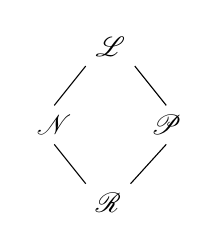
\begin{tikzpicture}[scale=0.5]
            \node (L) at (0,0) {$\mathscr{L}$};
            \draw (L.south west)--+(-0.8,-1) node[anchor=north] (N) {$\np$};
            \draw (L.south east)--+(0.8,-1) node[anchor=north] (P) {$\pp$};
            \draw (N.south)--+(0.8,-1) node[anchor=north west] (R) {$\rp$};
            \draw (P.south)--(R.north east);
        \end{tikzpicture}
        \caption{Partial order structure of outcome classes.}
        \label{fig: partial order structure}
    \end{figure}

    
    \begin{definition}
        Let $G$ and $H$ be short games. Then, $G\ge H$, if for all short games $X$, $$o(G+X)\ge o(H+X). $$
    \end{definition}
    Intuitively, $G \ge H$ means that $G$ is at least as favorable to Left as $H$.  
    While this definition captures the idea of game comparison, it is not practical for computation since the set of all games is infinite.  
    The following result, known as the \emph{Second Fundamental Theorem}, provides a more practical characterization when comparing games with the zero game.
    % The inequality $G \ge H$ means that $G$ is at least as favorable to Left as $H$. This definition of games inequality is not of practical use as the set of all games is an infinite set. The next theorem, which is the second fundamental theorem of CGT, gives a practical approach to compare a game with 0 game.
    
   \begin{theorem}[{\cite{S2013}*{Proposition~1.18}}]\label{thm: second fundamental theorem}
        Let $G$ be a short game. Then the following holds:
        \begin{itemize}
            \item $G=0 \Leftrightarrow o(G)=\mathscr{P}$,
            \item $G\ge 0 \Leftrightarrow o(G)\ge \mathscr{P}$,
            \item $G> 0 \Leftrightarrow o(G)=\mathscr{L}$,
            \item $G\le 0 \Leftrightarrow o(G)\le \mathscr{P}$,
            \item $G< 0 \Leftrightarrow o(G)= \mathscr{R}$,
            \item $G\cglfuz 0 \Leftrightarrow o(G)\le \mathscr{N}$,
            \item $G \cggfuz 0 \Leftrightarrow o(G)\ge \mathscr{N}$,
            \item $G\cgfuzzy 0 \Leftrightarrow o(G)= \mathscr{N}$.
        \end{itemize} 
    \end{theorem}

    % To compare two games, say, $G$ and $H$, we need inverse of a game with respect to disjunctive sum because if we have inverse of $H$, then we can compare $G+\text{Inv}(H)$ with 0 using the second fundamental theorem and then add $H$ on both the sides. The next definition gives us conjugate of a game and we will see that the conjugate of a game will serve as the inverse of that game.

    % To compare two games, say $G$ and $H$, we require the inverse of a game with respect to the disjunctive sum. If such an inverse of $H$ exists, say $\text{Inv}(H)$, then we can compare $G + \text{Inv}(H)$ with 0 game using theorem~\ref{}, and subsequently adding $H$ to both sides. 
    Using the second fundamental theorem, one can compare any game or disjunctive sum of games with 0. If inverse of a game is known with respect to the disjunctive sum, then any two games can be compared. % to compare two games, say $G$ and $H$, we can compare $G+\text{Inv}(H)$ with 0 using Theorem~\ref{thm: second fundamental theorem} and then add $H$ to both sides. 
    The following definition introduces the \emph{conjugate} of a game, which we shall see serves as the inverse of that game under disjunctive sum.
    % \ur{rewrite this without Inv and conjugate}
    \begin{definition}[Conjugate]
        Let $G$ be a short game. The conjugate of $G$, denoted by $\Bar{G}$, is defined recursively by $\Bar{G} = \{\Bar{G}^R\mid \Bar{G}^L\}.$
    \end{definition}

    Observe that the moves available to Left in a game $G$ are the same as those available to Right in its conjugate $\bar{G}$, and vice versa. Note that $\bar{G}$ is same as $-G$ defined in \cite{S2013}.


    \begin{theorem}[{\cite{S2013}*{Theorem~1.13}}]\label{thm:+ has inv}
        Let $G$ be a short game. Then $G+\bar{G}=0$.
    \end{theorem}
    Theorem~\ref{thm:+ has inv} implies that $\bar{G}$ is the inverse of $G$ under the disjunctive sum. This allows us to compare any two games.
    % Using these results, we get $\cgstar+\cgstar=0=\{-1\mid 1\}$ which tells that combinatorial games have many equivalent forms, but their actual forms are different in the sense that some options of a game might not be present in an equivalent game. For example: $\cgstar+\cgstar$ has an option $\cgstar$, but 0 does not have any option and the two games are still equal. We discuss this in detail in the next subsection.

     Using Theorem~\ref{thm: second fundamental theorem}, we obtain $\cgstar + \cgstar = 0$ as well as $\{-1 \mid 1\}=0$ as outcome of both $\cgstar+\cgstar$ and $\{-1\mid 1\}$ is $\pp$. This illustrates that combinatorial games can have multiple equivalent representations, even though their explicit forms are not identical. For instance, $\cgstar + \cgstar$ has an option $\cgstar$, whereas $0$ has no options, yet the two games are equivalent. We discuss this phenomenon in more detail in the next subsection.

    \subsection{Canonical Forms}\label{subsec: canonical form}
    As discussed above, every short combinatorial game $G$ may have several equivalent representations. This occurs because some options can be strategically inferior 
    % and will never be chosen by a rational player 
    while others may be overly advantageous. In this subsection, we show that every short game $G$ has a unique simplest form, called its \emph{canonical form}. The canonical form of a game is obtained by repeated application of two simplification rules: \emph{domination} and \emph{reversibility}.
    

    % \begin{definition}[Dominated and Reversible Options]
    % Let $G$ be a short game,\begin{itemize}
    %     \item A left option $G^{L_1}$ is dominated by $G^{L_2}$ if $G^{L_2}\ge G^{L_1}$ for some $G^{L_2}$.  
    %     (Interpretation: Left will prefer to play on $G^{L_2}$ because $G^{L_2}$ is more favorable to win of Left than $G^{L_1}$). Similar holds for Right. 
        
    %     \item A left option $G^{L_1}$ is reversible through $G^{L_1R_1}$ if $G^{L_1R_1}\le G$ for some Right option $G^{L_1R_1}$. 
    %     (Interpretation: if Left moves to $G^{L_1}$, then Right has a choice $G^{L_1R_1}$ which is equivalent or better for Right than the original game $G$, thus, Right would always prefer to move to $G^{L_1R_1}$). Similar holds for Right.   
    % \end{itemize}
    % \end{definition}

    \begin{definition}[Dominated and Reversible Options]
        Let $G$ be a short game.
        \begin{itemize}
            \item A Left option $G^{L_1}$ is \emph{dominated} by another Left option $G^{L_2}$ if $G^{L_2} \ge G^{L_1}$. The definition is symmetric for Right.
            
            \item A Left option $G^{L_1}$ is \emph{reversible} through a Right option $G^{L_1R_1}$ if $G^{L_1R_1} \le G$ for some $G^{L_1R_1} \in (G^{L_1})^{\mathscr{R}}$. The definition is symmetric for Right.
        \end{itemize}
    \end{definition}
    Intuitively, if $G^{L_1}$ is dominated by $G^{L_2}$, then Left will always prefer to move to $G^{L_2}$ rather than to $G^{L_1}$, since $G^{L_2}$ is at least as favorable to her as $G^{L_1}$. If $G^{L_1}$ is reversible, then after Left moves to $G^{L_1}$, Right can respond with $G^{L_1R_1}$, a position that is no worse (and possibly better) for Right than $G$ itself. Hence, After Left's move to $G^{L_1}$, Right will always move to $G^{L_1R_1}$.

    \begin{figure}[ht]
        \centering
        \begin{subfigure}[b]{0.40\textwidth}
        \centering
            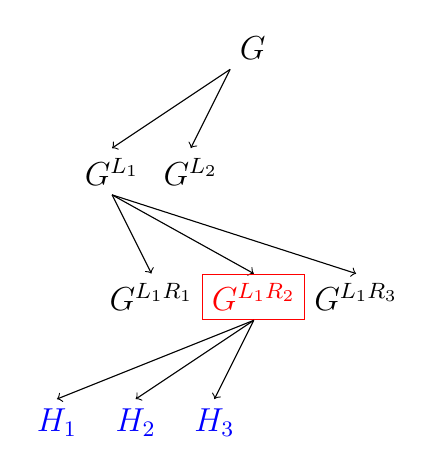
\begin{tikzpicture}[every node/.style={font=\large}]
        
                % Nodes
                \node (G) {$G$};
                \draw[->] (G.south west)--+(-1.5,-1) node[anchor=north] (GL) {$G^{L_1}$};
                \draw[->] (G.south west)--+(-0.5,-1) node[anchor=north] (GL1) {$G^{L_2}$};
                \draw[->] (GL.south)--+(0.5,-1) node[anchor=north] (GLR1) {$G^{L_1R_1}$};
                \draw[->] (GL.south)--+(1.8,-1) node[anchor=north, draw, red] (GLR2) {$G^{L_1R_2}$};
                \draw[->] (GL.south)--+(3.1,-1) node[anchor=north] (GLR3) {$G^{L_1R_3}$};
                \draw[->] (GLR2.south)--+(-0.5,-1) node[blue,anchor=north] (H3) {$H_3$};
                \draw[->] (GLR2.south)--+(-1.5,-1) node[blue,anchor=north] (H2) {$H_2$};
                \draw[->] (GLR2.south)--+(-2.5,-1) node[blue,anchor=north] (H1) {$H_1$};        
            \end{tikzpicture}
            \caption{Game tree of literal form of $G$}
        \end{subfigure}%
        \hspace{0em}%
        \begin{subfigure}[b]{0.40\textwidth}
        \centering
            \begin{tikzpicture}
                \node (G) {$G$};
                \draw[->] (G.south west)--+(-0.5,-1) node[anchor=north] (GL1) {$G^{L_2}$};
                \draw[->] (G.south west)--+(-1.5,-1) node[anchor=north,blue] (H3) {$H_3$};
                \draw[->] (G.south west)--+(-2.5,-1) node[blue,anchor=north] (H2) {$H_2$};
                \draw[->] (G.south west)--+(-3.5,-1) node[blue,anchor=north] (H1) {$H_1$};
                \draw[->,white] (H3)--+(0,-3.03) node (b) {};
            \end{tikzpicture}
            \caption{Game tree of simplified form of $G$ when $G^{L_1R_2}\le G$}
        \end{subfigure}
        \caption{Bypassing a reversible option. If $G^{L_1R_2}\le G$, then $G^L$ can be replaced by the set of all Left options of $G^{L_1R_2}$.}
        \label{fig: bypassing a reversible option}
    \end{figure}
    To simplify a game $G$, one can remove all dominated options of $G$. Moreover, if a left option $G^{L_1}$ is reversible through $G^{L_1R_1}$, then $G^{L_1}$ can be replaced by the left options of $G^{L_1R_1}$, as illustrated in Figure~\ref{fig: bypassing a reversible option}; an analogous rule applies to right options. By repeating this process of removing and replacing, one eventually obtains the simplest possible form of the game, known as the \textbf{canonical form} of $G$. This result follows from \cite{S2013}*{Theorems~2.4~and~2.5}.
    
    % To simplify a game $G$, one can remove all the dominated options of $G$ and if $G^{L_1}$ is reversible through $G^{L_1R_1}$, then $G^{L_1}$ can be replaced by the left options of $G^{L_1R_1}$ as shown in figure~\ref{fig: bypassing a reversible option} and vice-versa with right option.  This follows using {\cite{S2013}*{Theorem~2.4, Theorem~2.5}}

    \begin{example}
        Let $G = \uparrow + *$, where $\uparrow = \{0\mid *\}$. Then $ G=\{\uparrow+0, 0+*\mid \uparrow+0, *+*\} = \{\uparrow,*\mid \uparrow,0\}$. The canonical form of $G$ is $\{0,*\mid 0\}$.
    \end{example}

    The next subsection explores a particular type of game where neither player wants to start. %\ur{I suggest we follow instead our new conventions. What you call numbers here is better called zugzwangs. Numbers are the dyadics and the integers.}\an{We can make this change in the paper before submitting it anywhere, but for the thesis, I think we have to change a lot, because the same theory also goes into Robin hood paper.}

\subsection{Numbers and stops}
    Intuitively, a game is called a `Number' if each player prefers that the other player starts. 
    Recall that a {\em sub-position} of a game can be the game itself or any option of the game or any option of options, etc.

    \begin{definition}[Numbers]\label{def: Number}
     A short game $x$ is a Number if, in the canonical form of $x$, every sub-position $y$ satisfies $y^L<y^R$ for all $y^L$ and $y^R$.\footnote{The definition of a Number in \cite{S2013} does not hold for $\{*\mid*\}$ and many other literal form games that equal some canonical form Number.}
    \end{definition}

    The most basic Number games are integer games defined as follows: For all \( k \in \mathbb{Z}_{>0} \), the \emph{integer games} \( k \) and \( -k \) recursively defined as: 
    \begin{itemize}
        \item $k = \left\{ k-1 \mid \varnothing \right\}$;
        \item $-k = \left\{ \varnothing \mid -k+1 \right\}$,
    \end{itemize}
    where $0 = \{\varnothing \mid \varnothing \}$. 

    For all odd $k\in \Z$ and $n\in \Nat$, we define the {\em dyadic rational games} recursively as: $$ \frac{k}{2^n}=\left\{ \left[\frac{k-1}{2^n}\right] \mid \left[\frac{k+1}{2^n}\right] \right\},$$ 
    where the brackets denote the reduction of the fraction such that the numerator and denominator do not have a common divisor other than 1. For example, with $k=5$ and $n=1$, the game $5/2=\{2\mid 3\}$. We will call all integers and dyadic rationals simply as {\em dyadics} and denote the set of all dyadics by $\mathbb{D}$. As shown in \cite{S2013}*{Proposition 3.5} integer and dyadic rational games follow the standard arithmetic properties. 
    For instance, the disjunctive sum of the games $1$ and $\frac{1}{2}$ equals the game $1+\frac{1}{2}=\frac{3}{2}$. By definition, all dyadics are Numbers. 
    
    Let us restate a few theorems on Numbers. 

    \begin{theorem}[{\cite{S2013}*{Theorem~3.13}}]\label{thm: number avoidance}
        Let $x$ be a Number. If $G$ is not a Number then, $G+x=\{G^\mathcal L+x\mid G^\mathcal R+x\}$.
    \end{theorem}
    
   \begin{theorem}[{\cite{S2013}*{Theorem~3.7}}]\label{thm: archimedean principle}
       For any game $G$, there exists a positive integer $n$ such that $-n<G<n$.
   \end{theorem}

    Due to Theorem~\ref{thm: archimedean principle}, any game is smaller than large enough numbers and greater than small enough numbers. 
    The supremum of all numbers smaller than a given game $G$ is called the Right Stop of $G$ and similarly, the infimum of all numbers larger than $G$ is called the Left Stop of $G$. 
    % \begin{definition}[Confusion Interval]
    %     The confusion interval of a game is $\mathcal C(G)=\Set{x\in \mathbb D\SetSymbol G\cgfuzzy x}$
    % \end{definition}
    % The end points (supremum and infimum) of the confusion intervals are called {\em stops}. These can be easily described as follows:
    
    % \begin{definition}[Stops]\label{def: Left and Right stops}
    %     For a game $G$, the Left stop $\Ls(G)$ and the Right stop $\Rs(G)$ are:
    %     \begin{align*}
    %         \Ls(G)&=\begin{cases}
    %               x & \text{ if } G \text{ equals a dyadic } x;\\
    %               \max_{G^L} \left(\Rs(G^L)\right) & \text{ otherwise;}
    %         \end{cases}\\
    %         \Rs(G)&=\begin{cases}
    %               x & \text{ if } G \text{ equals a dyadic } x;\\
    %               \min_{G^R} \left(\Ls(G^R)\right) & \text{ otherwise.}
    %         \end{cases}   
    %     \end{align*}
    % \end{definition}
    % The stops of a game $G$ is the ordered pair $s(G)=(\Ls(G),\Rs(G))$.

    % The Left stop can also be interpreted as the maximum number of free moves Left can obtain in alternating play, when Left starts the game (this may be negative, if so, it is the minimum loss for Left). Similarly, the Right stop can be interpreted as the negative of the maximum number of free moves Right can obtain when Right starts the game (this may be positive).

    % We shall recall a few results about the stops from \cite{S2013} that will be of use to us later.

    % \begin{proposition}[{\cite{S2013}*{Proposition~3.17}}]\label{prop: relation between stop and game}
    %     Let $G$ be a game and let $x$ be a number. Then,
    %     \begin{enumerate}
    %     \item\label{item:prop: relation between stop and game:1} $\Ls(-G) = -\Rs(G)$ and $\Rs(-G) = -\Ls(G)$;
    %     \item\label{item:prop: relation between stop and game:2} if $G\geq x$, then $\Ls(G)\geq \Rs(G)\geq x$. Likewise if $G\leq x$ then, $\Rs(G)\leq \Ls(G)\leq x$;
    %     \item\label{item:prop: relation between stop and game:3} If $R(G) > x$, then $G > x$. Likewise, if $L(G) < x$, then $G < x$;
    %     \item $L(G) \text{ and } R(G) $ are the end points of $\mathcal C(G)$
    %     \end{enumerate}
    % \end{proposition}
    
    % \begin{proposition}[{\cite{S2013}*{Proposition~3.18}}]\label{prop: Lstop>Rstop}
    %     Let $G$ be a short game and let $x$ be any dyadic. Then, \begin{enumerate}
    %         \item\label{item:prop: Lstop>Rstop:1} $\Ls(G)\geq \Rs(G)$;
    %         \item\label{item:prop: Lstop>Rstop:2} $\Ls(G+x)=\Ls(G)+x$ and $\Rs(G+x)=\Rs(G)+x$.
    %         \item\label{item:prop: Lstop>Rstop:3} $L(G)\ge R(G^L)$ for every $G^L$ and $R(G)\le L(G^R)$ for every $G^R$, even if $G$ is equal to a number
    %     \end{enumerate}
    % \end{proposition}


    If a game is a Number, then both of its stops are equal; however, the converse does not hold. Games such as $*$ and $\cgup$ are not Numbers, yet both have Left and Right stops equal to $0$. This observation motivates the study of a broader class of games whose stops are both $0$ but which are not necessarily equal to $0$. These games are known as \emph{infinitesimals}. The next subsection explores such games and their properties in detail.
    
    \subsection{Infinitesimals}\label{subsec: infinitesimals}
    As mentioned above, infinitesimals are games whose Left and Right stops are both $0$. Before examining their structure and properties, we begin with a simpler subclass of games, namely the \emph{impartial} games, where both players have identical move options from every position.
    
    \begin{definition}[Impartial Game]
        A combinatorial game is \emph{impartial} if, from every subposition, both players have the same set of available moves.
    \end{definition}
    
    If a game $G$ is impartial, we do not distinguish between Left and Right options, since both players have identical choices from every position. 
    Hence, we represent an impartial game simply as $G = \{G_1, G_2, \dots, G_k\}.$

    A {\sc Nim} heap is an example of an impartial game and it is denoted by $*n$ where $n$ is the size of the heap and $*n=\{0,*,*2,\dots,*(n-1)\}$. These single-heap {\sc Nim} positions are called \textbf{nimbers}. As shown in \cite{S2013}*{Theorem~1.3}, every impartial game $G$ is equal to $*m$ for some non-negative integer $m$. 

    A related but more general class of games allows different sets of moves for each player, provided that at every subposition, either both players have available moves or neither does. 
    Such games are known as \emph{all-small} games. 
    % Impartial games form a special case of all-small games, and this broader class will play an important role in our discussion of infinitesimals.

    \begin{definition}[All-Small Games]
     A game is called all-small if, both players have available moves from every non-terminal subposition.
    \end{definition}
    
    Every impartial game is all-small, but the converse does not hold. For example, an instance of {\sc FS} with unequal positive wealths is all-small but not impartial.
    
    % As the name suggests, these games are small relative to dyadic rational games. Let $G$ be an all-small game, then for every positive dyadic rational $x$, $G$ satisfies $-x<G<x$. The idea of the proof is that Left always wins $G+x$ by keep playing on $G$. Similarly, Right always wins $G-x$ by keep playing in $G$. 
    % \sout{The terminology ``all-small'' also reflects the fact that these games are small in comparison to dyadics. Specifically,}
    If $G$ is an all-small game, then for every positive dyadic rational $x$, we have $ -x < G < x$. This inequality follows from the observation that in the game $G + x$, Left can secure a win by continually playing in $G$, while in $G - x$, Right can win by consistently playing in $G$.

    
   
    This property, however, is not limited to all-small games. Consider the game $H = \left\{ \left\{ 2 \mid 0 \right\} \mid 0 \right\}$. It satisfies  $-x < H < x$ for every positive dyadic rational $x$. But $H$ is not an all-small game as the subposition $2$ offers a move for Left but not for Right. This motivates a more general notion than all-small.
    
    \begin{definition}[Infinitesimal Game]
        A combinatorial game $G$ is called infinitesimal if, for every positive dyadic rational $x$, it satisfies $-x<G<x$.
    \end{definition}

  
    Returning to all-small games, the canonical forms of such games can be quite complex, as illustrated in Table~\ref{tab: cf of ts1(n;5,6)}. This complexity often makes it difficult to determine which player holds an advantage and to what extent. 
    
    % \sout{To quantify this advantage, we identify the simplest all-small game which provides an advantage to one of the players. Once this is known, we can use it to construct a scale of advantage, on which all all-small games can be positioned.}


    The simplest non-zero all-small game is $*=\{0\mid0\}$; it offers no advantage to either player, as first player wins this game. Notably, all-small games of the form $*n$, known as \emph{nimbers}%\sout{, corresponding to {\sc Nim} heaps,}
    , behave similar to $*$ in this context. %\sout{Hence, these games are not significant when considering the players' advantage.}
    
    The next simplest all-small game is Up, denoted $\cgup = \{0 \mid *\}$, which favors Left, as Left always wins this game. Its negative, called Down, denoted $\cgdown = \{* \mid 0\}$, favors Right.

    Since these are the simplest all-small games that confer an advantage to a player, it is reasonable to expect that any other all-small game which provides a player with an advantage must, in some sense, be comparable to these. Indeed, as shown in \cite{S2013}*{Theorem~4.8}, for every all-small game $G$, there is some $n$ such that $n\cdot\cgdown<G<n\cdot\cgup$, where $n\cdot\cgup$ denotes the disjunctive sum of $n$ copies of $\cgup$. This motivates the idea of evaluating the bound of advantage in an all-small game by %\sout{determining how many $\cgup$ or $\cgdown$ it is `equivalent' to} 
    determining minimum $n$ such that $n\cdot\cgdown<G<n\cdot\cgup$. But Conway gave a stronger notion that gives the exact advantage in an infinitesimal, especially all-small games, known as \emph{atomic weight}. Broadly, the atomic weight of a game is the number of copies of $\cgup$ ($\cgdown$, if negative), the game approximates.

    To pursue this idea, he gave a more flexible notion of equivalence than that given by canonical forms. %This notion consider two games as equivalent if they are indistinguishable in terms of how much they favor Left or Right. \ur{Improve this.}
    Recall that {\em birthday} of a game is the height of the game tree in its literal form. 

% This example shows that although nimbers do not favor any player, adding it to a game can change the players' advantage. The point to note that it happens only if the nimber being added to the game is already an option within the game. Therefore, while defining equivalence through the lens of nimbers, we must be cautious to exclude cases where the added nimber already appears as an option in the game. This motivates a more refined definition of equivalence using "sufficiently large" nimbers.}
    % % Let $G$ be a game that favors Left, i.e., $o(G)=\mathcal{L}$, and $n$ be a positive integer. Let us analyze the game $H=G+*n$. Since $o(*n)=\mathcal{N}$, $H$ is of the form $\mathcal{L}+\mathcal{N}$. Left wins as a first player on $H$ (by moving from $*n$ to $0$). If Right starts on $*n$, it can either move to $G+0$ or $G+*m$ where $m<n$. Left wins in both cases as $o(G)=\mathcal{L}$ and 0 is an option of $*m$. But if Right starts on $G$ and has a move to $*n$ from $G$, then Right wins by moving to $*n+*n$. So, although a nimber does not favor any player, adding it can alter the advantage if the nimber that is added to a game is also an option of the game. 

    
    % % we can try adding nimbers to an all-small game, and check whether it alters the players' advantage 
    
    % % It is well known that:
    % % \begin{itemize}
    % %     \item nimbers do not favor either player (first player wins $*n$ for $n>0$).
    % %     \item any move from nimbers is also a nimber from which a player can immediately move to 0,
    % % \end{itemize}
    % % Therefore, roughly speaking, when added to a game that provides advantage to a player, a nimber should not alter the advantage. But this is not true. for example, if $G=\cgup$, Left always wins $G$ but Right wins $G+*$ as first player. The reason is that the subposition $*$ of $G$ is the same as the nimber added. Therefore, a nimber, when added to a game that provides advantage to a player and has less birthday than that of the nimber, it should not alter the players' advantage. This motivates a natural definition of equivalence in this context: two games are considered equivalent if, for every third game $X$, their outcomes remain the same when combined with $X$ and nimbers of large enough birthdays.

    % % To do this, we require a more flexible notion of equivalence than the equivalence via canonical forms. We want to call two games equivalent if the amount of advantage both players have in the two game is the same. We know that nimbers do not favor either player, and thus should not alter the strategic advantage when added to a game. This suggests a natural equivalence definition in this context: two games are equivalent if their outcomes, when added to any third game $X$ along with nimbers, are the same.
    
    % % All we now need is a relaxed definition of `equivalent games' than `equivalence under canonical form' 
    % % as we are stuck in this problem because the canonical forms are complex. 
    % % As we already know, the nimbers do not favor any player and hence they do not change the advantage of Left or Right in the game, so, in this context, a natural definition of equivalence can be: if the outcome of two games in addition with any game $X$ in presence of nimbers is the same, then they are equivalent.

    % % But there is a slight problem with this definition. Consider two equal games $G$ and $H$, $G=\;\cgup\;=H$ , both games have equal advantage for Left as both are the same, but the games are not equivalent according to this new definition (if we take $X=0$, then $o(G+X+*)\neq o(H+X+*2)$). as per our intuition, the presence of any nimber should not change the advantage, but this is not what is happening in our example. The reason behind this is that $*$ is already present in $\cgup$. If instead of $*$, we had taken any large nimber, it would not have affected the outcome. So, we give a new definition of `equivalence'.

    % % However, there is a slight issue with this definition. Suppose $G =\; \cgup\; = H$. Both games clearly offers the same advantage to Left, as they are equal. Yet, under the proposed definition, they are not considered equivalent: for instance, if $X = 0$, then $o(G + X + *) \neq o(H + X + *2)$. Intuitively, the presence of any nimber should not affect the advantage, but we get a contradiction. This contradiction arises because $*$ is already a subposition of $\cgup$. If sufficiently large nimbers not present in either $G$ or $H$ were used instead, the discrepancy would not occur.
    
    % % This motivates the following refined notion of equivalence:

    % % \begin{definition}[Equivalence under $\cgfarstar$]
    % %     Two game $G$ and $H$ are said to be equivalent under $\cgfarstar$ if for any game $X$, $$o(G+X+\cgfarstar)=o(H+X+\cgfarstar).$$ Where $\cgfarstar$ denotes a large enough nimber which is not present in both $G$ and $H$.
    % % \end{definition}

    \begin{definition}[Equivalence under $\cgfarstar$]
        Two games $G$ and $H$ are said to be equivalent under $\cgfarstar$, denoted $\cgfarstareq{G}{H}$, if for every game $X$, ~$o(G + X + \cgfarstar) = o(H + X + \cgfarstar),$ where $\cgfarstar$ denotes a nimber of birthday larger than that of the games added to it.
    \end{definition}

    % The symbol $\cgfarstar$ denotes a large nimber, $\cgstar n$, that is not present in the game added to it. It suffices to select a nimber larger than the birthday of the game added to it. 
    % For example, for $\cgdoubleup+\cgfarstar$, $\cgfarstar$ could be set to be $*4$. If we have $G+\cgfarstar+\cgfarstar$ for some game $G$, then the first $\cgfarstar$ could be set to $*L_\beta$ such that $L_\beta$ is sufficiently large in the context of $G$ and the second $\cgfarstar$ could be set to $*N_\beta$ such that $N_\beta$ is sufficiently large in the context of $G+*L_\beta$.

    

    The following Theorem gives a practical way for checking whether two games are equivalent under $\cgfarstar$. For any positive integer~$n$, we denote the disjunctive sum of $n$ copies of~$\cgup$ by $n\cdot\cgup$, and $n\cdot\cgup+\cgfarstar$ by $n\cdot\cgup\;\cgfarstar$. When $n=1$, we write $\cgup\;\cgfarstar$ for $1\cdot\cgup+\cgfarstar$. Similar conventions apply to~$\cgdown$.
    
    % Note that for any positive integer $n$, we denote disjunctive sum of $n$ copies of $\cgup$ by $n\cdot\cgup$,  $n\cdot\cgup+\cgfarstar$ by $n\cdot\cgup\;\cgfarstar$ and if $n=1$, $1\cdot\cgup+\cgfarstar$ is denoted by $\cgup\;\cgfarstar$ and use similar notations for $\cgdown$.

    \begin{theorem}[{\cite{LiP}*{Theorem~9.30}}]\label{thm: check farstareq}
        For two games $G$ and $H$, $\cgfarstareq{G}{H}$ if and only if $~\cgdown\;\cgfarstar<G-H<\;\cgup\;\cgfarstar$.
    \end{theorem}
    % If we play $\cgup$ with any large nimber $*n$, then also it is advantageous for Left, to define this, we first provide an equivalence relation
    % To resolve this issue, a relaxed equivalence, `Equivalence under $\cgfarstar$', of games is introduced which captures the important part of infinitesimal games. 
    % In many cases, it happens that an infinitesimal game consists of a simple dominant (or biggest) infinitesimal and a more complicated error term. If we know the dominant part of a number of infinitesimal games, then this is frequently sufficient information to determine the outcome of their sum.
    
    % The next step to compute the advantage of players in a game is to find out how many Ups or Downs a game is equivalent to, this is essentially the same as finding out an integer $w$ for a game $G$ such that $\cgfarstareq{G}{w\cdot\cgup}$. This $w$ is called the atomic weight of $G$. 
    
    Having established this relaxed equivalence relation, the next step in understanding players' advantage is to estimate how many copies of $\cgup$ or $\cgdown$ a given all-small game equals. In other words, for a game $G$, we wish to find a game $w$ such that $\cgfarstareq{G}{w \cdot \cgup}$ where $w \cdot \cgup$ denotes the `norton product' and in case $w$ is an integer, it is the disjunctive sum of $w$ copies of $\cgup$ when $w > 0$, and $|w|$ copies of $\cgdown$ when $w < 0$. It turns out that if the there exists such a  game $w$, it is unique, and it is referred to as the \emph{atomic weight} of $G$.

    % \begin{definition}[Atomic Weight]\label{def: atomic weight}
        % For a game $G$, if $\cgfarstareq{G}{w\cdot\cgup}$, then $w$ is called the atomic weight of $G$, and is denoted by $\aw(G)=w$. \footnote{Not all games have an integer atomic weight; in some cases, the atomic weight of a game is itself a game. For further details, see \cite{LiP} and \cite{S2013}.}
    % \end{definition}

    \begin{definition}[Atomic Weight]\label{def: atomic weight}
        For a game $G$, if $\cgfarstareq{G}{w\cdot\cgup}$, for some game $w$, then $G$ is atomic, and the atomic weight of $G$ is  $\aw(G)=w$. \footnote{For further details, see \cites{LiP,S2013}.}
    \end{definition}
    
    If $w = \aw(G)$ is positive, then Left has an advantage in $G$; if $w$ is negative, then Right has an advantage in $G$, which is more precisely stated in Theorem~\ref{thm: outcome using aw}.
    % If $w=\aw(G)$ is positive (negative), Left (Right) has advantage in $G$, and $w.\cgup$ is defined as $w$ copies of $\cgup$ ($\cgdown$) in disjunctive sum. 
    % If $w$ is negative, Right has advantage in $G$ and $w.\cgup$ is defined as $w$ copies of $\cgdown$ in disjunctive sum.

    % The other way of looking at the atomic weight is as follows: We know that Left (Right) has one move advantage in $\cgup$ ($\cgdown$), that is, Left (Right) can wait for one Right (Left) move before Right wins the game and the atomic weight of a game is same as the number of $\cgup$ ($\cgdown$) a game is equivalent to. This gives a new interpretation of atomic weight and that is: the atomic weight a game is the number of moves a player can wait in that game before the other player makes the winning move.
    
    Another way to interpret atomic weight is through {\em delayed} moves. We know that $\cgup$ offers Left a one move waiting  advantage, that is, Left can afford to wait through one Right move and still win, while $\cgdown$ offers the same advantage to Right.  Whenever the atomic weight of a game corresponds to the number of $\cgup$ or $\cgdown$ it is equivalent to, we can interpret the atomic weight as the number of moves a player can wait in the game before the opponent secures a win. Note that this interpretation is correct only when the atomic weight is larger than one. The atomic weight of $\cgup+\cgstar=\{0,*\mid 0\}$ is one but Left does not have a waiting  advantage, but  instead she has a parity advantage.

    
    % While Theorem~\ref{thm: check farstareq} and Definition~\ref{def: atomic weight} combinedly give a way to check whether $w$ is the atomic weight of $G$ or not, but gives no way to find the atomic weight of $G$. The following Theorem from \cite{LiP} give a way to compute atomic weight of a game.
    The next few lemmas play an important role in computation of atomic weight of games.
    
   \begin{lemma}[{\cite{S2013}*{Page~139}}]\label{lem: n-cgup-cgfarstar}
        For any positive integer $n$, $$n\cdot\cgup\;\cgfarstar=\{0\mid (n-1)\cdot\cgup\;\cgfarstar\} \text{ and } n\cdot\cgdown\;\cgfarstar=\{(n-1)\cdot\cgdown\;\cgfarstar\mid0\}$$
    \end{lemma}

    \begin{lemma}[\cite{S2013}*{Proposition~7.12}]\label{lem: aw of sum of games}
        Let $G$ and $H$ be atomic, then \begin{enumerate}
            \item $\aw(-G)=-\aw(G)$;
            \item $\aw(G+H)=\aw(G)+\aw(H)$.
        \end{enumerate}
    \end{lemma}
    
    \begin{lemma}[Atomic Weight of Nimbers]\label{lem: aw of nimbers}
        The atomic weight of a nimber is 0.
    \end{lemma}
    \begin{proof}
          By Definition~\ref{def: atomic weight}, it is sufficient to prove that $\cgfarstareq{*n}{0\cdot \cgup}$, which is simply the same as $\cgfarstareq{*n}{0}$. According to Theorem~\ref{thm: check farstareq}, this is equivalent to verify the inequality:
        \[
        \cgdown\;\cgfarstar < *n < \cgdown\;\cgfarstar.
        \]  We will prove the left inequality, $\cgdown\;\cgfarstar<*n$; the proof of the right one is analogous. 
        
        To prove $\cgdown\;\cgfarstar<*n$, we must show $\cgdown\;\cgfarstar-*n\in \rp$. Here, $\cgfarstar+*n\;(=\cgfarstar-*n)$ is equivalent to $\cgfarstar$ as both are nimbers and $\cgfarstar$ is a large nimber. Therefore the game becomes $\cgdown + \cgfarstar$, which is equal to $\{\cgfarstar\mid 0\}$, by lemma~\ref{lem: n-cgup-cgfarstar}. If Right starts, he wins by moving to 0. If Left starts, she moves to $\cgfarstar$ from where Right can move to 0 and win.
        % \begin{itemize}
        %     \item If Right moves first, he can play from $\cgfarstar$ to $0$, reducing the game to just $\cgdown$. Since $\cgdown < 0$, Right wins.
        %     \item If Left moves first, she can either move to $\cgdown+*m$ for $m\geq 0$, or to $*+\cgfarstar$. In the former case, if $m>0$, Right wins by moving to $\cgdown$ and if $m=0$, Right wins as $\cgdown<0$. In the later case, Right wins by moving from $\cgfarstar$ to $*$ as $*+*=0$.
        % \end{itemize}
    \end{proof}

    
    While Theorem~\ref{thm: check farstareq} and Definition~\ref{def: atomic weight} together provide a way to verify whether a given integer $w$ is the atomic weight of a game $G$, they do not offer a method to compute the atomic weight directly. The following theorem from \cite{LiP}, provides a way to determine the atomic weight of an all-small game. Note that it also establishes that each all-small games is atomic, i.e. that they all have well defined atomic weight. There are infinitesimal games that do not have atomic weight, for example.

    \begin{theorem}[{\cite{LiP}*{Theorem~9.39}}]\label{thm: compute aw}
        Let $G$ be all-small. If $G=\{G^L\mid G^R\}$ and $G^L$ and $G^R$ have atomic weights, then the atomic weight of $G$ is given by $\left\{ \aw(G^L)-2\mid\aw(G^R)+2\right\}$ unless this is an integer. In that case, let $x$ be the least integer such that $\aw(G^L)-2\cglfuz x$, and $y$ the greatest integer such that $y\cglfuz \aw(G^R)+2$.
        \begin{itemize}
            \item If $G\cgfuzzy \cgfarstar$, $\aw(G)=0$;
            \item If $G>\cgfarstar$, $\aw(G)=y$;
            \item If $G<\cgfarstar$, $\aw(G)=x$.
        \end{itemize}
    \end{theorem}

The next Theorem helps to determine the outcome of a game if its atomic weight in known. The second rule is commonly known as the ``two-ahead-rule''.

\begin{theorem}[\cite{S2013}*{Theorem~7.13}]\label{thm: outcome using aw}
    Let $G$ be atomic. Then
    \begin{enumerate}
        \item if $\aw(G)=1$, then $G\cggfuz 0$;
        \item if $\aw(G)\ge 2$, then $G>0$.
    \end{enumerate}
\end{theorem}
This concludes the CGT basics needed to read and understand the paper.

   % This concludes the section. In the next section, we present the canonical form of {\sc FS}.

%%%%%%%%%%%%%%%%%%%%%%%%%%%%%%%%%%%%%%%%%%%%%%%%%%%%%%%%%%%%%%%%%%%%%%%%%%%%%%%%%%%%%%%%%%%%%%%%%%%%%%%%%%%%%%%%%%%%%%%%%%%%%%%%%%%%%%%%%%%%%%%%%%%%%%%%%%%%%%%%%%%%%%%%%%%%%%%%%%%%%%%%%%%%%%%%

\bibliographystyle{plain}
\begin{thebibliography}{9}
\bibitem{LiP} Albert, M., Nowakowski, R. and Wolfe, D., 2019. {\em Lessons in play: an introduction to combinatorial game theory}. AK Peters/CRC Press.
\bibitem{BDL} Balachandran, N., Dargad, A. and Larsson, U., 2026. Temperatures of Robin Hood. {\em The Electronic Journal of Combinatorics}, pp.P2-32.
\bibitem{BCG2004} Berlekamp, E.R., Conway, J.H. and Guy, R.K., 2004. {\em Winning ways for your mathematical plays}, volume 4. AK Peters/CRC Press.
\bibitem{DHNP} Duchêne, E., Heinrich, M., Nowakowski, R. and Parreau, A., 2022. Partizan subtraction games, {\em Integers, Combinatorial Game Theory: A Special Collection in Honor of Elwyn Berlekamp, John H. Conway and Richard K. Guy}, p.121.
\bibitem{FA} Fraenkel, A.S. and Kotzig, A., 1987. Partizan octal games: partizan subtraction games. {\em International Journal of Game Theory}, 16(2), pp.145-154.
\bibitem{M} Mesdal III, G.A., 2005. Partizan splittles. In {\em Games of No Chance III}, Proc. BIRS Workshop on Combinatorial Games (pp. 447-461).
\bibitem{LMNS} Larsson, U., McKay, N.A., Nowakowski, R.J. and Siegel, A.A., 2018. Wythoff partizan subtraction. {\em International Journal of Game Theory}, 47(2), pp.613-652.
\bibitem{URYCG2020} Larsson, U., Meir, R. and Zick, Y., 2020. Cumulative Games: Who is the current player?.  Preprint arXiv:2005.06326.
\bibitem{S2013} Siegel, A.N., 2023. {\em Combinatorial game theory} (Vol. 146). American Mathematical Society.
\end{thebibliography}

\end{document}
